% arara: pdflatex
% arara: bibtex
% arara: pdflatex
% arara: clean: {files: [thesis.aux, thesis.bbl, thesis.blg, thesis.bcf, thesis.lof, thesis.log, thesis.lot, thesis.out, thesis.run.xml, thesis.toc, thesis-blx.bib]}

\documentclass{scrbook} % <= Druckversion: "scrbook", Bildschirmversion: "scrreprt"
\newcommand\bcor{8mm} % <= falls nötig, Bindungskorrektur für Druckversion (ohne Layoutzerstörung bei Anpassung)
\usepackage{osm-thesis}
\usepackage[space]{grffile} % allow spaces in graphics file name (even if it has no `.<file extension>`)
\usepackage{tikz} % draw graphs
\usetikzlibrary{shapes,arrows,fit,backgrounds,decorations.pathreplacing}
\usepackage{todonotes}
\setlength{\marginparwidth}{2cm}
\usepackage{tikzpeople}
\usepackage{pifont} % checkmarks \cmark
\usepackage{booktabs} % table lines 
\usepackage{threeparttable}
\usepackage{colortbl}

%\usepackage{footnote} % footnotes in envs
%\makesavenoteenv{figure}
%\makesavenoteenv{tabular}

%deeper lists
\usepackage{enumitem}
\setlistdepth{9}
\setlist[itemize,1]{label=$\bullet$}
\setlist[itemize,2]{label=$\bullet$}
\setlist[itemize,3]{label=$\bullet$}
\setlist[itemize,4]{label=$\bullet$}
\setlist[itemize,5]{label=$\bullet$}
\setlist[itemize,6]{label=$\bullet$}
\setlist[itemize,7]{label=$\bullet$}
\setlist[itemize,8]{label=$\bullet$}
\setlist[itemize,9]{label=$\bullet$}
\renewlist{itemize}{itemize}{9}

% fix http://tex.stackexchange.com/questions/311426/bibliography-error-use-of-blxbblverbaddi-doesnt-match-its-definition-ve/311428
\makeatletter
\def\blx@maxline{77}
\makeatother

% multiple figures next to each other
\usepackage{subcaption}

% sidewaysfigure environment
\usepackage{rotating}

% ABOUT
\newcommand{\hpitype}{Master's Thesis}
\newcommand{\hpiauthor}{Fredrik Teschke}
\newcommand{\hpititle}{Securing Legacy Applications with Intel SGX}
\newcommand{\hpititleother}{Absichern von Legacy Anwendungen mit Intel SGX} % <= das Studienreferat verlangt einen deutschen UND englischen Titel
\newcommand{\hpisupervisor}{Prof.\,Dr.\,Andreas Polze, Max Plauth}
\newcommand{\hpichair}{Operating Systems and Middleware Group}
\newcommand{\hpiexternalsupervisor}{}
\newcommand{\hpiexternal}{}
\newcommand{\hpidate}{\today}
\newcommand{\hpihpi}{Hasso-Plattner-Institut at the University of Potsdam}

% DOCUMENT
%\KOMAoption{draft}{true} % <= z.B. zum "Debuggen" der Overfull-Boxes
\bibliography{bibliography}

\begin{document}
        %\hypersetup{hidelinks}
	\selectlanguage{english}

	% Einband
	\pagenumbering{alph}
	\ifisbook\begin{titlepage}
	\setlength{\evensidemargin}{0.5\evensidemargin+0.5\oddsidemargin}
	\setlength{\oddsidemargin}{\evensidemargin}

	\centering

	\raisebox{-0.5\height}{
\includegraphics[width=5.5cm]{images/hpi_logo_black.pdf}}
	\hspace*{.2\textwidth}
	\raisebox{-0.5\height}{
\includegraphics[width=4cm]{images/uni_logo_black.pdf}}
	

	\vspace*{4\baselineskip}
	{\usekomafont{subject}\hpitype}\par
	\vspace*{2\baselineskip}
	{\usekomafont{title}\hpititle\par}
	\vspace*{\baselineskip}
	{\usekomafont{subtitle}\hpititleother}\par
	\vspace*{2\baselineskip}
	{\usekomafont{author}\hpiauthor}\par
	
	\vfill
	
	{\usekomafont{date}\hpihpi}\par
	\vspace*{\baselineskip}
	{\usekomafont{date}\hpidate}\par
	
\end{titlepage}\fi
	\ifisbook\cleardoubleemptypage\fi

	% (Haupt-)Titelseite, Abstract, ggf. Danksagung & Inhaltsverzeichnis
	\pagenumbering{roman}
	\begin{titlepage}
	\centering

	\raisebox{-0.5\height}{
\includegraphics[width=5.5cm]{images/hpi_logo_srgb.pdf}}
	\hspace*{.2\textwidth}
	\raisebox{-0.5\height}{
\includegraphics[width=4cm]{images/uni_logo_srgb.pdf}}

	\vspace*{4\baselineskip}
	{\usekomafont{subject}\hpitype}\par
	\vspace*{2\baselineskip}
	{\usekomafont{title}\hpititle\par}
	\vspace*{\baselineskip}
	{\usekomafont{subtitle}\hpititleother}\par
	\vspace*{2\baselineskip}
	{\usekomafont{author}\hpiauthor}\par

	\vfill
	{\textbf{Supervisors}\\\usekomafont{publishers}\hpisupervisor\\\textit{\hpichair}\\\smallskip\textbf{\normalfont\hpiexternalsupervisor}\\\textit{\hpiexternal}}

	\vspace*{2\baselineskip}
	{\usekomafont{date}\hpihpi}\par
	\vspace*{\baselineskip}
	{\usekomafont{date}\hpidate}\par

	\setcounter{page}{1}

\end{titlepage}


	\ifisbook\cleardoubleemptypage\fi% => Wenn die Arbeit auf Deutsch verfasst wurde, verlangt das Studienreferat KEINEN englischen Abstract

% % englischer Abstract
%
\begin{otherlanguage}{english}
\begin{center}\textsf{\textbf{Abstract}}\end{center}

\noindent
The release of Intel SGX revived the interest in trusted computing across industry and academia.
Hardware is available, but usage patterns and applications are mostly missing.
This thesis evaluates trusted computing from the viewpoint of a software engineer.
Hardening strategies are identified in related work and applied in two case studies.
The case studies show how SGX can be used in practice. A small helper library is developed for rapid prototyping.
Other trusted computing solutions are compared to SGX and SGX is critically evaluated based on current research.
\end{otherlanguage}

\vspace{2cm}


% => Wenn die Arbeit auf Englisch verfasst wurde, verlangt das Studienreferat einen englischen UND deutschen Abstract

% deutsche Zusammenfassung
\begin{otherlanguage}{ngerman}
\begin{center}\textsf{\textbf{Zusammenfassung}}\end{center}

\noindent
Die Veröffentlichung von Intel SGX hat das Interesse an Trusted Computing in Akademia und Industrie wieder erweckt.
Obwohl die Hardware verfügbar ist, sind Verwendungsmuster and Anwendungen noch Mangelware.
Diese Arbeit evaluiert Trusted Computing aus der Sicht eines Software Ingenieurs.
In verwandten Arbeiten werden Strategien zum Härten von Anwendungen identifiziert und in zwei Fallstudien angewandt.
Diese Fallstudien zeigen wie SGX praktisch genutzt werden kann. Dabei wird eine kleine Hilfs-Bibliothek entwickelt.
Andere Trusted Computing Lösungen werden mit SGX verglichen und SGX wird mit Hilfe aktueller Forschungsergebnisse kritisch bewertet.
\end{otherlanguage}




	%\ifisbook\cleardoubleemptypage\fi\include{content/dedication}
	\tableofcontents
	\cleardoublepage

	% Textteil
	\pagenumbering{arabic}
	


% color definitions
\colorlet{greenbg}{green!50!white}
\colorlet{redbg}{red!50!white}
\colorlet{orangebg}{orange!50!white}
% styles
%\tikzstyle{block} = [rectangle, draw, align=center, rounded corners]
%\tikzstyle{line} = [draw, -latex']
%\tikzstyle{legend} = [nodes={anchor=base}, column sep=5pt, row %sep=5pt, yshift=-2cm, anchor=north]
%\tikzstyle{legend heading} = [gray]
%\tikzstyle{heading} = [minimum height=0.2cm]
%\tikzstyle{edge label} = [midway, above, minimum width=0]
%\tikzstyle{myperson} = [minimum size=40pt, person]
%\tikzstyle{computer} = [draw, dotted]

% lengths
\newlength{\haloOffset}
\newlength{\personOffset}
\setlength{\haloOffset}{13pt}
\setlength{\personOffset}{3pt}
\definecolor{bluekeywords}{rgb}{0.13,0.13,1}
\definecolor{greencomments}{rgb}{0,0.5,0}
\definecolor{redstrings}{rgb}{0.9,0,0}

\lstdefinestyle{default-base}{
  breaklines=true,
  postbreak=\mbox{\textcolor{red}{$\hookrightarrow$}\space},
  numbers=left,
  xleftmargin=5ex,
  basicstyle=\footnotesize\ttfamily,
  commentstyle=\color{greencomments},
  keywordstyle=\color{bluekeywords}\bfseries,
  stringstyle=\color{redstrings},
}
\lstdefinestyle{default}{
  style=default-base,
  morekeywords={uint32_t, uint8_t, sgx_aes_ctr_128bit_key_t, size_t, sgx_sealed_data_t, sgx_lib_encrypted_data_t, int64_t, FILE, sgx_status_t, sgx_enclave_id_t, enclave, trusted, untrusted, from, import, include, in, out, size, readonly, string, user_check, diff, wget},
  keywordsprefix=\#,
  alsoletter=\#,
}
\lstdefinestyle{cpp}{
  language=C++,
  style=default
}
\lstdefinestyle{edl}{
  style=cpp,
}
\lstdefinelanguage{diff}{
  morecomment=[f][\color{bluekeywords}]{@@},     % group identifier
  morecomment=[f][\color{redstrings}]-,         % deleted lines
  morecomment=[f][\color{greencomments}]+,       % added lines
  morecomment=[f][\color{magenta}]{---}, % Diff header lines (must appear after +,-)
  morecomment=[f][\color{magenta}]{+++},
}
\lstdefinelanguage{hex}{
    morecomment=[l]{//},
}
\newcommand{\rot}[1]{\makebox[1em][l]{\rotatebox{45}{#1}}}
\newcommand{\h}[1]{\textbf{\rot{#1}}}
\newcommand{\cmark}{\ding{51}}

\chapter{Introduction\label{ID_1883383221}}
Cloud computing has proven itself as a viable and popular business model.\label{ID_698884812}
This makes data security an increasingly hot topic.\label{ID_1630969494}
Encryption as a way of securely transporting data is an age-old and proven concept.\label{ID_1712713994}
By comparison, techniques for secure data \textit{processing} are still in their infancy.\label{ID_718488027}

For some decades there have been niche solutions in this field called trusted computing. They did not gain the traction and publicity they may have deserved. Among such solutions are Trusted Platform Modules and ARM's TrustZone security extensions.\label{ID_853445864}
Now Intel has joined the game and has been shipping its Security Guard Extensions (SGX) with many of its new CPUs since end of 2015.\label{ID_563845396}
The wide-spread availability of trusted computing hardware is foreseeable. There is a growing demand for trustworthy applications in digital rights management and cloud computing. This means the game might soon begin to change, shifting trusted computing back into focus.\label{ID_1881143424}

From a technological standpoint, trusted computing is fascinating. It combines the fields of cryptography, operating systems and hardware design.\label{ID_1778003077}
However, from an ethical standpoint, trusted computing is a double-edged sword as \autoref{figure:tc-cartoon} pointedly makes clear.\label{ID_1885832293}
\begin{figure}[htbp]
\makebox[\textwidth][c]{
	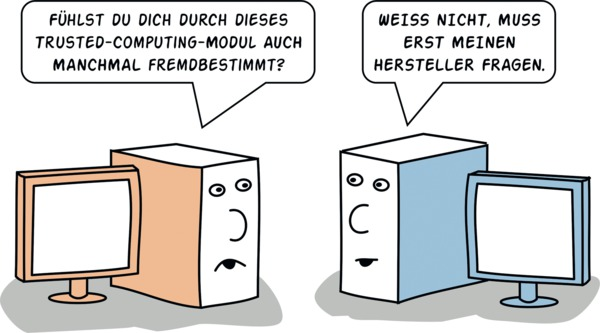
\includegraphics[width=0.7\textwidth]{content/images/trusted computing cartoon}
}\caption{\textbf{Trusted computing cartoon.} Left computer: ``Do you also sometimes feel remotely controlled by this trusted computing module?''. Right computer: ``I don't know, let me ask my manufacturer.'' Reprinted from \cite{ix-enclave}.\label{ID_863606381}\label{figure:tc-cartoon}\label{ID_863606381}\label{figure:tc-cartoon}}
\end{figure}


Intel SGX, and with it the field of trusted computing in general, still has to pick up traction. Yet the technology is ready for being used and evaluated today.\label{ID_1141283910}
A variety of research is happening around SGX, and innovative use cases are popping up.\label{ID_970909799}

This thesis looks at trusted computing from a \textit{software engineer's perspective}.\label{ID_889066539}
The goal of this thesis is to show how a developer can harden his applications today, using the technology that is available.\label{ID_128655856}
The thesis is mainly made up of literature work.\label{ID_941979765}
Techniques for secure remote computation are described, among them trusted computing (\autoref{chapter:background}).\label{ID_1961860825}
A wide variety of trusted computing solutions is then surveyed and systematically compared (\autoref{chapter:tc-solutions}). Both commercial solutions and research work are included.\label{ID_1378520845}

Intel SGX is chosen as the prime candidate for a more detailed evaluation (\autoref{chapter:sgx}).\label{ID_33539746}
The SDK provided by Intel is presented along with a small helper library that was developed as part of this thesis (\autoref{chapter:sgx-lib}).\label{ID_1352179523}
Architectural design patterns for hardening applications are identified in the related work (\autoref{chapter:related-work}).\label{ID_1745973426}
Two case studies show how database software -- representative for the class of hosted applications -- can be hardened using Intel SGX (\autoref{chapter:kissdb}, \autoref{chapter:sqlite}).\label{ID_148600996}
These case studies use the patterns and techniques found in related work.\label{ID_916299114}

While SGX is an exciting technology that is in many regards better than previous solutions, it is far from perfect.\label{ID_1005742561}
Criticism and security issues are also presented.\label{ID_1799898232}

The source code for this thesis -- including all text, images and code snippets -- is available at \url{https://github.com/ftes/sgx-thesis}.\label{ID_1636604444}

\chapter{Background\label{ID_941070001}\label{chapter:background}}
Nowadays, data is oftentimes not stored -- and applications are not executed -- locally (on premise) any more. Rather, these tasks are outsourced to hosted, remote infrastructure. In addition, computer technology is becoming increasingly pervasive in our lives. More data is stored on and processed by computers, making them ever more valuable targets.\label{ID_1470188624}
\begin{figure}[htbp]
\makebox[\textwidth][c]{% node distance: vertical and horizontal
\begin{tikzpicture}[
    node distance=0.5cm and 4cm, auto,
    nodes={{minimum height=0.7cm, text width=2cm}},
    block/.style={rectangle, draw, align=center, rounded corners},
    line/.style={draw, -latex'},
    legend/.style={nodes={anchor=base}, column sep=5pt, row sep=5pt, yshift=-2cm, anchor=north},
    legend heading/.style={gray},
    heading/.style={minimum height=0.2cm},
    edge label/.style={midway, above, minimum width=0},
    myperson/.style={minimum size=40pt, person},
    computer/.style={draw, dotted},
    secure/.style={fill=greenbg},
    insecure/.style={fill=redbg}
]
    % Place nodes
    \node [                  block          ] (input)   {1. input};
    \node [right=of input,   block, secure  ] (store1)  {3. store}; 
    \node [below=of store1,  block, insecure] (process) {4. process};
    \node [below=of process, block, secure  ] (store2)  {5. store};
    \node [left=of store2,   block          ] (output)  {7. output};
    \node [above=of input,   heading        ] (client)  {Client};
    \node [above=of store1,  heading        ] (server)  {Server};
   
    % Draw edges
    \path [line] (input)   -- (store1) node [edge label, secure] {2. transmit};
    \path [line] (store1)  -- (process);
    \path [line] (process) -- (store2);
    \path [line] (store2)  -- (output) node [edge label, secure] {6. transmit};
   
    % Fit cluster edges
    \node [computer, inner sep=10pt, fit=(input) (output) (client)] (client fit) {};
    \node [computer, inner sep=10pt, fit=(store1) (process) (store2) (server)] (server fit) {};
   
    % Legend
    %\matrix[legend] (legend) at (current bounding box.south) {
    %    \node[secure,   align=center] {considered solved\\(encryption)}; &
    %    \node[insecure, align=center] {considered unsolved\\(focus of this thesis)}; \\
    %};
   
    % Cluster headings
    %\node[heading, legend heading] at (legend.north) {Legend};
\end{tikzpicture}

}\caption{\textbf{Focus of this thesis within the data life cycle.}\label{ID_1160378356}
Transmitting and storing data can be secured using encryption (green). The applications examined in this thesis deal with processing data (red). This is an area of active research.\label{ID_745166579}
\label{ID_671023153}\label{figure:data-lifecycle}}
\end{figure}

The state of the art is to protect sensitive data by \textit{encrypting} it while it is at rest or being transmitted. This is shown in \autoref{figure:data-lifecycle}.\label{ID_1880219695}
Protecting the processing stage is an active field of research called \textit{secure remote computation}.\label{ID_1852842699}
\begin{figure}[htbp]
\makebox[\textwidth][c]{\begin{tikzpicture}[
    node distance=15pt and 170pt, auto,
    nodes={{minimum size=4cm, minimum height=0.6cm}},
    trim right=(remote computer fit.east), trim left=(data owner fit.west),
    block/.style={rectangle, draw, align=center, rounded corners},
    line/.style={draw, -latex'},
    legend/.style={nodes={anchor=base}, column sep=5pt, row sep=5pt, yshift=-2cm, anchor=north},
    legend heading/.style={gray},
    heading/.style={minimum height=0.2cm},
    edge label/.style={midway, above, minimum width=0},
    myperson/.style={minimum size=40pt, person},
    computer/.style={draw, dotted}
]
    % Place nodes
    \node [block, draw=none, heading] (remote computer)   {Remote Computer};
    \node [block, below=of remote computer] (untrusted software)   {Untrusted Software};
    \node [block, draw=none, below=of untrusted software, heading] (container)   {Trusted Execution\\Environment};
    \node [block, below=of container] (code) {Private Code};
    \node [block, below=of code] (data) {Private Data};
    \node [block, draw=none, left=of remote computer, heading] (data owner) {Data Owner's Computer};
    \node [block, left=of code] (setup) {Setup};
    \node [block, below=of setup] (verification) {Verification};
    \node [block, draw=none, above=of setup, heading] (dispatcher) {Computation Dispatcher};

	% Fits
    \node [draw, inner sep=10pt, fit=(dispatcher) (setup) (verification)] (dispatcher fit) {};
    \node [computer, inner sep=10pt, fit=(dispatcher fit) (data owner)] (data owner fit) {};
    \begin{scope}[on background layer]
        \node [draw, inner sep=10pt, fit=(container) (code) (data), fill=greenbg] (container fit) {};
    \end{scope}
    \node [computer, inner sep=10pt, fit=(container fit) (untrusted software) (remote computer)] (remote computer fit) {};

    % Draw people
    \node[myperson, below=of data owner fit, yshift=-30pt] (data owner person) {Data Owner};
    \node[myperson, evil, below=of remote computer fit, yshift=-30pt] (remote computer owner person) {Infrastructure Owner};
    \node[myperson, good] at ($(data owner person)!0.5!(remote computer owner person)$) (software provider) {Software Provider};

    % Draw edges
    \path [line] (dispatcher fit.20) -- (container fit.west |- dispatcher fit.20) node [edge label] {Setup Computation};
    \path [line] (container fit.180) -- (dispatcher fit.east |- container fit.180) node [edge label] {Receive Encrypted Results};
    \path [line] ($(data owner person.north)+(0,\personOffset)$) -- (data owner fit) node [edge label, left] {Trusts, Owns};
    \path [line] ($(remote computer owner person.north)+(0,\personOffset)$) -- (remote computer fit) node [edge label, right] {Manages};
    \path [line] ($(software provider.north)+(0,\haloOffset)$) |- (dispatcher fit.330) node [edge label] {Authors};
    \path [line] ($(software provider.north)+(0,\haloOffset)$) |- (dispatcher fit.330 -| container fit.west) node [edge label] {};
    \path [line] (data owner person) -- (software provider) node [edge label] {Trusts};   
\end{tikzpicture}

}\caption{\textbf{Secure remote computation.}\label{ID_1573575704}
The data owner trusts the software provider but not the infrastructure owner. The code and data within the trusted execution environment (green) must be protected. There are different options for implementing this protection.\label{ID_532436106}
Reprinted from \cite{sgx-explained}.\label{ID_28551827}
\label{ID_50207747}\label{figure:secure-remote-computation}}
\end{figure}

\autoref{figure:secure-remote-computation} gives an abstract overview of the entities and steps involved in secure remote computation. For the sake of this thesis, the most interesting part of the picture is the implementation of the container.\label{ID_1217277821}

Arasu et al.\@ categorise the approaches for constructing such a container that can protect code and data on a remote computer:\cite[p. 19]{querying-encrypted-data-tutorial}\label{ID_500367217}
\begin{description}\label{ID_27140838}
\item[Compute on encrypted data] The data remains encrypted during processing. Thus the results are also encrypted. In this case the cryptographic scheme is the container. No information about the plain text should be leaked. \autoref{crypto} explains which encryption schemes support this.\label{ID_328666411}
\item[Decrypt and process data in a secure location] Such a location could be a local machine, disconnected from the internet, or a remote trusted hardware component such as a secure co-processor. Whether or not a location is deemed secure is a subjective decision. This variant of implementing the container is called \textit{trusted computing}.\label{ID_481899872}
\end{description}\label{ID_933485978}
The remainder of this chapter explains the fundamental concepts of both these approaches.\label{ID_1721841145}

Implementations of the first approach are presented later on in \autoref{section:secure-db}.\label{ID_1199323088}
Implementations of trusted computing are described and compared in \autoref{chapter:tc-solutions}.\label{ID_684830290}
Intel SGX -- a particular commercial solution for trusted computing -- is described in more detail in \autoref{chapter:sgx}.\label{ID_733461445}

\section{Cryptography\label{ID_265480959}\label{crypto}}
There are several different ways in which cryptographic principles can be used to implement the concept of a secure container.\label{ID_544485861}
\begin{description}\label{ID_958111314}
\item[Multi party computing]\label{ID_1564094585}
Several parties jointly compute a function to which every party provides some input. The input of each party is not revealed to any of the other parties. One early implementation is Yao's garbled circuits.\cite[]{Gupta}\label{ID_1507598191}
For secure remote computation, we could assume two parties, where only the data owner provides an input and only the infrastructure owner executes the function.\label{ID_1818312817}
However, the function output is in plain text which is not desirable for secure remote computation in general.\label{ID_647862117}
\item[Verifiable computing]\label{ID_1000386877}
This is a first step in the direction of secure remote computing. It ensures the integrity but not the confidentiality of the computation (similar to a cryptographic signature).\cite{Gennaro2010,Karapanos,Vu2013}\label{ID_1343830016}
\item[Homomorphic Encryption]\label{ID_1769833687}
Such encryption schemes define calculation operations on encrypted data. The operands and result of these calculations remain encrypted so they could be performed by an untrusted third party.\label{ID_1952238538}
\autoref{figure:homomorphic-encryption} explains the principle of homomorphic encryption with an example. While partially homomorphic schemes define only one operation (e.g. either addition or multiplication), fully homomorphic schemes define both.\label{ID_1116118751}
\begin{figure}[htbp]
\makebox[\textwidth][c]{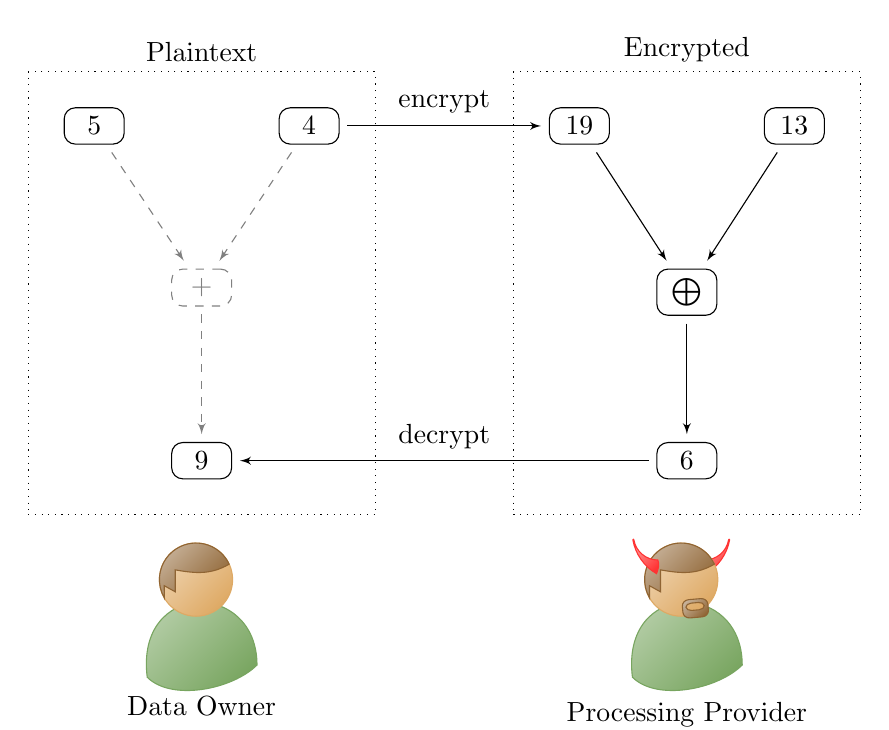
\begin{tikzpicture}[
    auto,
    node distance=40pt and 50pt,
    nodes={{minimum height=0.6cm}},
    block/.style={rectangle, draw, align=center, rounded corners},
    line/.style={draw, -latex'},
    legend/.style={nodes={anchor=base}, column sep=5pt, row sep=5pt, yshift=-2cm, anchor=north},
    legend heading/.style={gray},
    heading/.style={minimum height=0.2cm},
    edge label/.style={midway, above, minimum width=0},
    myperson/.style={minimum size=40pt, person},
    computer/.style={draw, dotted},
    number/.style={block, text width=1.5em, minimum size=1em, outer sep=3pt},
    indirect/.style={draw=gray, dashed, gray}
]
    % Place nodes
    \node [number]                (five) {5};
    \node [number, right=of five] (four) {4};
    \node at ($(five)!0.5!(four)$) (center) {};

    \node [number, right=of four, xshift=20pt] (five enc) {19};
    \node [number, right=of five enc] (four enc) {13};
    \node at ($(five enc)!0.5!(four enc)$) (center enc) {};

    \node [number, below=of center, indirect] (plus) {$+$};
    \node [number, below=of center enc] (plus enc) {$\bigoplus$};
    \node [number, below=of plus enc] (sum enc) {6};
    \node [number] at (center |- sum enc) (sum) {9};
  
    % Fit cluster edges
    \node [computer, inner sep=10pt, fit=(five) (four) (sum)] (plaintext) {};
    \node [computer, inner sep=10pt, fit=(five enc) (four enc) (sum enc)] (encrypted) {};

    % Headings
    \node [heading, anchor=south] at (plaintext.north) {Plaintext};
    \node [heading, anchor=south] at (encrypted.north) {Encrypted};

    % Draw people
    \node[myperson, below=of plaintext, yshift=30pt] (data owner) {Data Owner};
    \node[myperson, evil, below=of encrypted, yshift=30pt] (remote owner) {Processing Provider};

    % Draw edges
    %\draw [decoration={brace, raise=5pt}, decorate] ($(four.north east)+(0,2pt)$) -- ($(four.south east)+(0,-2pt)$) node [pos=0.5, outer sep=3pt] (brace) {};
    \path [line, indirect] (five) -- (plus);
    \path [line, indirect] (four) -- (plus);
    \path [line, indirect] (plus) -- (sum);
    \path [line] (five enc) -- (plus enc);
    \path [line] (four enc) -- (plus enc);
    \path [line] (plus enc) -- (sum enc);
    \path [line] (four) -- (five enc) node [edge label] {encrypt};
    \path [line] (sum enc) -- (sum) node [edge label] {decrypt};
\end{tikzpicture}


}\caption{\textbf{Homomorphic encryption example.}\label{ID_610399076}
A homomorphic encryption scheme defines operations on encrypted data. The decrypted result of the encrypted addition ($\bigoplus$) gives the same result as performing a plain text addition ($+$). Using this scheme an untrusted \textit{processing provider} can perform calculations without learning anything about the plain text.\label{ID_1072580727}
\label{ID_1989105116}\label{figure:homomorphic-encryption}}
\end{figure}

Gentry et al. successfully constructed the first fully homomorphic scheme in 2009.\cite[]{Gentry2009}\label{ID_233387469}
\autoref{figure:encryption-schemes} shows the relationship between different encryption schemes and the operations they support. These schemes are revisited in \autoref{section:secure-db}, which also shows how they can be practically put to use.\label{ID_129969722}
\begin{figure}[htbp]
\makebox[\textwidth][c]{\begin{tikzpicture}[
    tight fit/.style={inner sep=0pt, outer sep=0pt},
    block/.style={rectangle, draw, align=center, rounded corners},
    line/.style={draw, -latex'},
    legend/.style={nodes={anchor=base}, column sep=5pt, row sep=5pt, yshift=-2cm, anchor=north},
    legend heading/.style={gray},
    heading/.style={minimum height=0.2cm},
    edge label/.style={midway, above, minimum width=0},
    myperson/.style={minimum size=40pt, person},
    computer/.style={draw, dotted}
]

% base matrix
\matrix (first) [every node/.style={text width=4cm, minimum height=1.5cm, align=center}, row sep=0.2cm, column sep=0.2cm]
{
\node (A1) {}; & \node (A2) {}; & \node (A3) {}; \\
\node (B1) {}; & \node (B2) {}; & \node (B3) {}; \\
\node (C1) {}; & \node (C2) {}; & \node (C3) {}; \\
\node (D1) {}; & \node (D2) {}; & \node (D3) {}; \\
};

% nodes
% text in fit nodes is not vertically centered - use an additional node
\node (order) at (B3) {order-preserving ($\geq$)};
\node (det) at (C3) {deterministic ($==$)};
\node[draw, fit=(A1) (A2) (A3), tight fit, fill=redbg]   (fully)    {}; \node (fully text)    at (fully) {fully homomorphic};
\node[fit=(B1) (C1), tight fit,]                         (paillier) {}; \node (paillier text) at (paillier) {Paillier \cite{Paillier1999} ($+$)};
\node[fit=(B2) (C2), tight fit]                          (elgamal)  {}; \node (elgamal text)  at (elgamal) {ElGamal \cite{ElGamal1985} ($\times$)};
\node[draw, fit=(D1) (D2) (D3), tight fit, fill=greenbg] (non det)  {}; \node (non det text)  at (non det) {non-deterministic ($\emptyset$)};
\begin{scope}[on background layer]
\node[draw, fit=(paillier) (elgamal), tight fit, fill=orangebg] (partially) {};
\node[draw, fit=(B3) (C3), tight fit, fill=greenbg] {};
\end{scope}
\node[anchor=north west] at (partially.north west) {partially homomorphic};

% paths
\path[line] (non det text)  -- (paillier text);
\path[line] (non det text)  -- (elgamal text);
\path[line] (non det text)  -- (det);
\path[line] (det)      -- (order);
\path[line] (paillier text) -- (fully text);
\path[line] (elgamal text)  -- (fully text);
\path[line, dashed] (order)    -- (fully text);
\end{tikzpicture}

}\caption{\textbf{Encryption schemes and their relationships.}\label{ID_489936542}
The shading indicates computational efficiency (red: impractical, orange: expensive, green: practical). Arrows indicate subsumption of functionality. Fully homomorphic schemes for example provide both $+$ and $\times$ operations (and by extension -- e.g. an encrypted CPU -- also comparison operations).\label{ID_1527882742}
Reprinted from \cite{querying-encrypted-data-tutorial}.\label{ID_467588759}
\label{ID_452615921}\label{figure:encryption-schemes}}
\end{figure}

State of the art fully homomorphic schemes still suffer from an intractably high overhead. Partially homomorphic schemes on the other hand have already been applied to databases.\cite{Baumann2014,querying-encrypted-data-tutorial}\label{ID_1599544022}

Encryption schemes in themselves also do not help verify what computation took place. Combining encryption with verifiable computation approaches or software attestation may provide a solution.\label{ID_717622838}
\item[Encrypted CPU]\label{ID_1403278513}
Given a (fully) homomorphic encryption scheme it is possible to execute entire encrypted programs. This is possible in a fully oblivious fashion where both the instruction flow and memory access (code and data) remain hidden.\label{ID_601974181}
Both obliviousness and the current fully homomorphic encryption schemes incur such large performance penalties that they are not yet practically useful for more complex programs.\label{ID_312856627}

The encrypted CPU works very much the same as a regular CPU, as can be seen in \autoref{figure:encrypted-cpu}. A regular CPU operates on bits using logical gates. The encrypted CPU operates on encrypted bits. Each bit is represented by cipher value of $n$ bits size so that there are $2^{n-1}$ possible representations for $0$ and $1$ respectively. Logical gates are emulated using the fully homomorphic operations on these cipher values (addition and multiplication).\cite[]{Brenner2011}\label{ID_1020198095}
\begin{figure}[htbp]
\makebox[\textwidth][c]{
	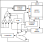
\includegraphics[width=0.6\textwidth]{content/images/encrypted cpu}
}\caption{\textbf{Encrypted CPU schematic.} This is a classic von-Neumann architecture where the memory holds both the instructions and data. Bits are represented as encrypted numbers. Reprinted from \cite{Brenner2011a}.\label{ID_901443426}\label{figure:encrypted-cpu}\label{ID_901443426}\label{figure:encrypted-cpu}}
\end{figure}

Both code and data reside in the encrypted memory. This means that code and data remain secret at all times.\label{ID_1323926141}

The circuit evaluation provides \textit{obliviousness} as the entire circuit must always be solved. For example, on memory accesses each cell is reassigned -- either with its new value on a write, or an equivalent representation of its old bit value.\label{ID_818872921}
This obliviousness is an important security factor and a performance pitfall at the same time. Memory access patterns and program flow are kept secret. This however also means that access times grow with the memory size. The authors state that ``compact programs and data are the key to tolerable runtimes''.\cite[]{Brenner2012}\label{ID_1325928179}

A hardware implementation of the encrypted CPU has not yet been attempted due to various challenges such as super-wide buses and the recrypt procedure necessitated by the encryption scheme.\label{ID_1008727172}
A software implementation highlights the performance problems. Without encryption, a CPU cycle is simulated in $3 ms$. With encryption this value increases to $166 s$.\label{ID_1078829631}
\footnote{This is the measurement for the highest value of the security parameter $lambda$. Unfortunately, neither Brenner et al. nor Smart et al.\cite{Smart2010} give further details on how the security parameter relate to a comparable security level. The BSI advises a security level of $120 bit$ from the year 2022 onwards: \url{https://www.bsi.bund.de/SharedDocs/Downloads/DE/BSI/Publikationen/TechnischeRichtlinien/TR02102/BSI-TR-02102.pdf}.}\label{ID_1789113343}
Both values are obtained for $256$ memory rows -- at $13 bit$ per row this gives roughly $0.4 kB$ of memory.\footnote{A memory word contains $8 bit$ of data and a $5 bit$ command.\cite{Brenner2011}. This design decision reduces the number of costly memory access cycles.}\cite[]{Brenner2012}\label{ID_1799557031}
\end{description}\label{ID_408605672}

Fully homomorphic encryption adds another tool to a cryptographer's toolbox: The ability to compute on encrypted data. The concept of an encrypted CPU builds on top of this primitive. It shows how a encrypted program with branching can be executed on encrypted data.\label{ID_1875507588}

The performance of fully homomorphic schemes is still far from being practically applicable. Through the oblivious full-circuit evaluation of the encrypted CPU this issue is amplified. However, improvements are possible on several avenues:\label{ID_607327069}
New, more efficient fully homomorphic schemes may be devised. The existing schemes can be optimised both in their algorithm and in their implementation (e.g. parallelised). Hardware implementation of the encryption, and especially the encrypted CPU also has large potential benefits.\label{ID_262947221}

Yet even a sufficiently efficient encrypted CPU could not solve secure remote computation once and for all. Firstly the computation is restricted to a single client. Without decrypting the results (in a trusted location) no communication and interaction between clients is possible. Secondly the problem of attestation is not solved by this approach.\label{ID_295590508}

\section{Trusted Computing\label{ID_360935729}\label{section:tc}}
This section defines terms important for trusted computing. These are most relevant for \autoref{chapter:tc-solutions}.\label{ID_1527667001}
\begin{description}\label{ID_1233402803}
\item[Root of trust]\label{ID_854088737}
is the sole element on which trust in a platform hinges. If the root of trust is compromised, the whole platform is compromised.\cite[]{Mitchell2005}\label{ID_1888900657}
For example, the CPU in a trusted computing setup could be the root of trust that is expected to function correctly.\label{ID_871944257}
\item[Trusted computing]\label{ID_1657615964}
is a form of secure remote computation that uses trusted hardware as the root of trust.\cite[]{Mitchell2005}\label{ID_1723503487}
\autoref{figure:trusted-computing} shows the involved components and trust relationships.\label{ID_535952528}
\item[Trusted Execution Environment (TEE)]\label{ID_261824335}
protects its assets (such as code and data) from attacks. It usually exists alongside the standard Rich Execution Environment (REE).\cite[]{GlobalPlatform}\label{ID_1872162923}
The TEE is at the very heart of a trusted computing implementation as shown in \autoref{figure:trusted-computing}. This section describes different TEE implementations.\label{ID_530801514}
\item[Trusted computing base (TCB)]\label{ID_1719015402}
is best described by the \textit{Orange Book}: The TCB ``contains all of the elements of the system responsible for supporting the security policy''.\cite[]{orangebook}\label{ID_1237482443}
This includes the root of trust, the application itself, and all intermediate software levels that have to be trusted.\label{ID_143606732}
Anything outside of the TCB does not have to be trusted.\label{ID_1731344432}
The TCB should be as small and simple as possible for the sake of security.\cite[]{orangebook}\label{ID_294862822}
Depending on the trusted computing solution the TCB may contain the operating system and/or the hypervisor.\label{ID_962329179}
\item[Software Attestation] is a two-part process. First a loaded piece of software is measured to ensure that the system is in a well-defined state. Secondly, this measurement is cryptographically signed and transmitted. This protocol can be enriched to include a key exchange. This makes it possible to securely communicate with the attested code. The process is described well in \cite{sgx-explained}.\label{ID_372928242}
\item[Data Sealing] is a process of storing data so that it can only be accessed by a component in a certain state. For example, bank account credentials could be sealed so that they can only be read by a certain operating system at a certain patch-level.\cite[]{Mitchell2005}\label{ID_708201927}

Technically, this is usually achieved through key derivation. The root of trust in a system may have a secret key. From this key, with the measurement result of software attestation, a state-specific data sealing key is derived. The data is then encrypted with this key.\label{ID_1904605343}
\end{description}\label{ID_242504118}
\begin{figure}[htbp]
\makebox[\textwidth][c]{% makebox for over-wide figure   
\makebox[\linewidth]{
\begin{tikzpicture}[
  node distance=15pt and 170pt, auto,
  nodes={{minimum width=3.5cm, minimum height=0.6cm}},
  trim right=(manufacturer.east),
  trim left=(data owner fit.west),
  block/.style={rectangle, draw, align=center, rounded corners},
  line/.style={draw, -latex'},
  legend/.style={nodes={anchor=base}, column sep=5pt, row sep=5pt, yshift=-2cm, anchor=north},
  legend heading/.style={gray},
  heading/.style={minimum height=0.2cm},
  edge label/.style={midway, above, minimum width=0},
  myperson/.style={minimum size=40pt, person},
  computer/.style={draw, dotted},
  new/.style={font=\bfseries}
]
  % Place nodes
  \node [block, draw=none] (remote computer) {Remote Computer};
  \node [block, draw=none, new, below=of remote computer] (trusted hardware)  {Trusted Hardware};
  \node [block, below=of trusted hardware] (untrusted software)  {Untrusted Software};
  \node [block, draw=none, below=of untrusted software] (container)  {Trusted Execution\\Environment};
  \node [block, below=of container] (code) {Private Code};
  \node [block, below=of code] (data) {Private Data};

  \node [block, left=of code] (setup) {Setup};
  \node [block, below=of setup] (verification) {Verification};
  \node [block, draw=none, above=of setup] (dispatcher) {Computation Dispatcher};
  \node [block, draw=none] at (remote computer -| setup) (data owner) {Data Owner's Computer};
 
  % Fit cluster edges
  \node [draw, inner sep=10pt, fit=(dispatcher) (setup) (verification)] (dispatcher fit) {};
  \node [computer, inner sep=10pt, fit=(dispatcher fit) (data owner)] (data owner fit) {};
  \begin{scope}[on background layer]
    \node [draw, inner sep=10pt, fit=(container) (code) (data), fill=greenbg] (container fit) {};
  \end{scope}
  \node [draw, inner sep=10pt, fit=(container fit) (untrusted software) (trusted hardware)] (trusted hardware fit) {};
  \node [computer, inner sep=10pt, fit=(trusted hardware fit) (remote computer)] (remote computer fit) {};

  % Draw people
  \node[myperson, below=of data owner fit, yshift=-30pt] (data owner person) {Data Owner};
  \node[myperson, evil] (remote computer owner person) at (data owner person -| remote computer fit) {Infrastructure Owner};
  \node[myperson, good] at ($(data owner person)!0.5!(remote computer owner person)$) (software provider) {Software Provider};
  \node[myperson, good, right=of remote computer owner person, xshift=-100pt, new] (manufacturer) {Manufacturer};

  % Draw edges
  \path [line] (dispatcher fit.20) -- (container fit.west |- dispatcher fit.20) node [edge label] {Setup Computation};
  \path [line] (container fit.180) -- (dispatcher fit.east |- container fit.180) node [edge label] {Receive Encrypted Results};
  \path [line] ($(data owner person.north)+(0,\personOffset)$) -- (data owner fit) node [edge label, left] {Trusts, Owns};
  \path [line] ($(remote computer owner person.north)+(0,\personOffset)$) -- (remote computer fit) node [edge label, right] {Manages};
  \path [line] ($(manufacturer.north)+(0,\haloOffset)$) |- (trusted hardware fit) node [edge label, new] {Builds};
  \path [line] ($(software provider.north)+(0,\haloOffset)$) |- (dispatcher fit.330) node [edge label] {Authors};
  \path [line] ($(software provider.north)+(0,\haloOffset)$) |- (dispatcher fit.330 -| container fit.west) node [edge label] {};
  \path [line] (data owner person) -- (software provider) node [edge label] {Trusts};
  \path [line] ($(data owner person.south)+(0,-0.5)$) -- +(0,-1.0) -- ($(manufacturer.south)+(0,-1.5)$) node [edge label, new] {Trusts} -- ($(manufacturer.south)+(0,-0.5)$);
\end{tikzpicture}
}

}\caption{\textbf{Trusted computing.}\label{ID_1038375068}
The trusted execution environment is protected by trusted hardware. This introduces an additional trust relationship. Additional nodes (compared to \autoref{figure:secure-remote-computation}) are in bold font.\label{ID_1467217011}
Reprinted from \cite{sgx-explained}.\label{ID_1474157281}
\label{ID_1792311294}\label{figure:trusted-computing}}
\end{figure}


\chapter{Trusted Computing Solutions\label{ID_309872773}\label{chapter:tc-solutions}}
As explained, trusted computing is a variant of secure remote computing built on trusted hardware.\label{ID_1898011333}
This chapter first defines metrics for classifying trusted computing implementations.\label{ID_268617658}
Commercially available solutions and solutions from research are then described qualitatively.\label{ID_1980391789}
Finally, a more quantitative comparison is given in form of a table. It uses the defined metrics as the main criteria.\label{ID_1605459160}

\section{Classification\label{ID_979419236}}
The following dimensions are used to classify the solutions presented in the remainder of this section:\label{ID_1876235781}
\begin{description}\label{ID_385656837}
\item[Hardware implementation] (if present). \autoref{figure:tee} shows a variety of approaches ranging from external to on-chip solutions as defined by the GlobalPlatform alliance.\cite[]{GlobalPlatform}\label{ID_205762418}
Using hardware virtualisation techniques is a fourth option used in some solutions.\label{ID_472468399}
\item[Isolation level] at which the TEE protects the components. \autoref{figure:tee-granularity} shows the five predominant isolation levels. These levels can be observed repeatedly when evaluating the trusted computing implementations presented in this thesis.\label{ID_466621036}
\end{description}\label{ID_1293092830}
\begin{figure}[htbp]
\makebox[\textwidth][c]{% makebox for over-wide figure   
\makebox[\linewidth]{
\begin{tikzpicture}[
  scale=0.8, transform shape,
  nodes={text width=2cm, draw, minimum height=1cm, align=center},
  tee/.style={fill=greenbg},
  subtitle/.style={font=\bfseries, draw=none, text width=}
]
    % external
	\node (v1) at (-3,1.5) {RAM};
	\node (v2) at (-3,-0.5) {ROM};
	\node (v4) at (0,-0.5) {Internal peripherals};
	\node (v3) at (0,1.5) {Processing core(s)};
	\draw (-4.5,3) rectangle (1.5,-1.5);
	\node[draw=none] at (-1.5,2.5) {SoC};
	\node (v5) at (0,4) {External memory};
	\node (v7) at (-3,4) {External peripherals};
	\node[text width=, tee] (v6) at (-1.5,-2.5) {External Security SoC};
	\draw  (-4,0.5) -- (1,0.5);
	\draw  (v1) |- (-3,0.5);
	\draw  (v2) |- (-3,0.5);
	\draw  (v3) |- (0,0.5);
	\draw  (v4) |- (0,0.5);
	\draw  (v5) |- (0,3);
	\draw  (v7) |- (-3,3);
	\draw  (v6) |- (-1.5,-1.5);
	\node[subtitle] at (-1.5,-4) {a) External secure element};
	
	\draw[dashed]  (2.25,5) -- (2.25,-4.5);
	
	% embedded
	\node (v1b) at (4.5,1.5) {RAM};
	\node (v2b) at (4.5,-0.5) {ROM};
	\node (v4b) at (7.5,-0.5) {Internal peripherals};
	\node (v3b) at (7.5,1.5) {Processing core(s)};
	\draw (3,3) rectangle (9,-3);
	\node[draw=none] at (6,2.5) {SoC};
	\node (v5b) at (7.5,4) {External memory};
	\node (v7b) at (4.5,4) {External peripherals};
	\node[text width=, tee] (v6b) at (6,-2) {On-SoC security subsystem};
	\draw  (3.5,0.5) -- (8.5,0.5);
	\draw  (v1b) |- (4.5,0.5);
	\draw  (v2b) |- (4.5,0.5);
	\draw  (v3b) |- (7.5,0.5);
	\draw  (v4b) |- (7.5,0.5);
	\draw  (v5b) |- (7.5,3);
	\draw  (v7b) |- (4.5,3);
	\draw  (v6b) |- (6,0.5);
	\node[subtitle] at (6,-4) {b) Embedded secure element};
	
	\draw[dashed]  (9.75,5) -- (9.75,-4.5);
	
	% processor
	\node (v1c) at (12,1.5) {RAM};
	\node (v2c) at (12,-0.5) {ROM};
	\node (v4c) at (15,-0.5) {Internal peripherals};
	\node (v3c) at (15,1.5) {Processing core(s)};
	\draw (10.5,3) rectangle (16.5,-1.5);
	\node[draw=none] at (13.5,2.5) {SoC};
	\node (v5c) at (15,4) {External memory};
	\node (v7c) at (12,4) {External peripherals};
	\draw  (11,0.5) -- (16,0.5);
	\draw  (v1c) |- (12,0.5);
	\draw  (v2c) |- (12,0.5);
	\draw  (v3c) |- (15,0.5);
	\draw  (v4c) |- (15,0.5);
	\draw  (v5c) |- (15,3);
	\draw  (v7c) |- (12,3);
	\node[subtitle] at (13.5,-4) {c) Processor secure environment};
	
	
	% TEE elements
	\begin{scope}[on background layer]
		\path[tee] (v5b.90) rectangle (v5b.south east);
		
		\path[tee] (v1c.90) rectangle (v1c.south east);
		\path[tee] (v2c.90) rectangle (v2c.south east);
		\path[tee] (v3c.90) rectangle (v3c.south east);
		\path[tee] (v4c.90) rectangle (v4c.south east);
		\path[tee] (v5c.90) rectangle (v5c.south east);
		\path[tee] (v7c.90) rectangle (v7c.south east);
	\end{scope}
\end{tikzpicture}
}

}\caption{\textbf{Implementation alternatives for protecting a Trusted Execution Environment (TEE) as defined by the GlobalPlatform alliance.}\label{ID_1049041551}
The logic necessary to protect the TEE lives in nodes shaded green. It can either reside outside of the System on a Chip (SoC) as in \textit{a)}, or as a part of the regular SoC components as in \textit{c)}.\label{ID_377511617}
Reprinted from \cite{GlobalPlatform}.\label{ID_1243979231}
\label{ID_1516783594}\label{figure:tee}}
\end{figure}

\begin{figure}[htbp]
\makebox[\textwidth][c]{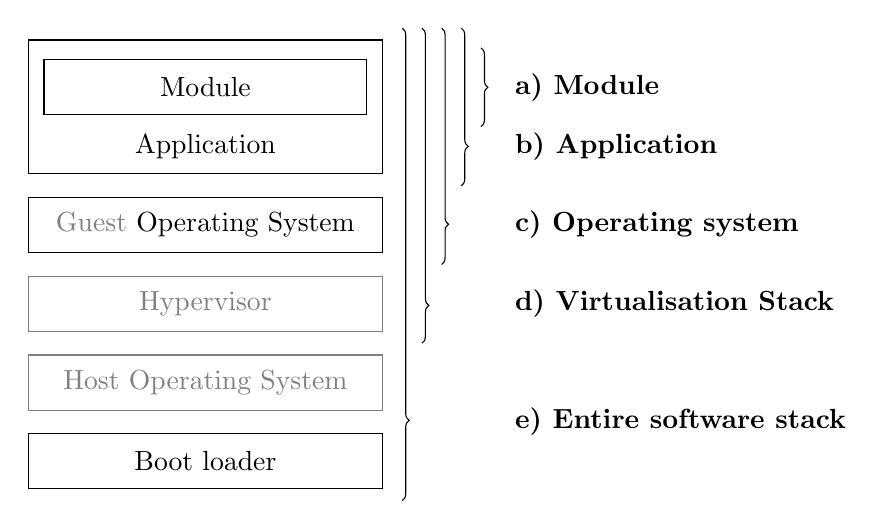
\begin{tikzpicture}[
  nodes={draw, text width=4.5cm, inner sep=0, minimum height=0.7cm, align=center},
  optional/.style={color=gray, draw=gray},
  label/.style={draw=none, align=left, inner sep=5pt, font=\bfseries, text width={}, align=left}
]

\node (bl) at (-0.5,-1.5) {Boot loader};
\node [optional] (os1) at (-0.5,-0.5) {Host Operating System};
\node [optional] (hyp) at (-0.5,0.5) {Hypervisor};
\node (os2) at (-0.5,1.5) {\textcolor{gray}{Guest} Operating System};
\node [draw=none] (app) at (-0.5,2.5) {Application};
\node [text width=4.1cm] (mod) at (-0.5,3.25) {Module};
\draw (-2.75,3.85) rectangle (1.75,2.15);

\node [label, right] at (3.25,3.25) {a) Module};
\draw[decorate, decoration={brace, mirror}] (3,2.75) -- (3,3.75);

\node [label, right] at (3.25,2.5) {b) Application};
\draw[decorate, decoration={brace, mirror, aspect=0.25}] (2.75,2) -- (2.75,4);

\node [label, right] at (3.25,1.5) {c) Operating system};
\draw[decorate, decoration={brace, mirror, aspect=0.17}] (2.5,1) -- (2.5,4);

\node [label, right] at (3.25,0.5) {d) Virtualisation Stack};
\draw[decorate, decoration={brace, mirror, aspect=0.12}] (2.25,0) -- (2.25,4);

\node [label, right] at (3.25,-1) {e) Entire software stack};
\draw[decorate, decoration={brace, mirror, aspect=0.17}] (2,-2) -- (2,4);

\end{tikzpicture}

}\caption{\textbf{Possible levels of isolation a Trusted Execution Environment (TEE) can provide.}\label{ID_1446907066}
\textit{a)} -- \textit{e)} represent the five predominant levels in the evaluated trusted computing solutions. Virtualisation is not employed by all solutions, therefor the \textit{host operating system} and \textit{hypervisor} are printed in grey.\label{ID_1739628616}
\label{ID_1112289760}\label{figure:tee-granularity}}
\end{figure}


\section{Commercial\label{ID_1886048225}}
The following list of commercial trusted computing solutions gives a good overview of how the field has evolved in the past 15 years.\label{ID_642511098}
The list is not exhaustive. Instead, the chosen solutions represent noteworthy archetypes.\footnote{The most noticeable omission from this list are all kinds of cryptographic co-processors that aim to provide significant computational resources apart from the main CPUs. Any operation in excess of cryptographic primitives such as key generation and digital signatures is considered significant.} For a more extensive list, see \cite{tee_mobile_devices}.\label{ID_727374297}
\begin{description}\label{ID_838567667}
\item[2002: Trusted Platform Module (TPM)\footnotemark]\label{ID_878785835}
\footnotetext{TPM hardware first became available for the revision 1.2 of the TPM specification. This was published in 2003: \url{https://trustedcomputinggroup.org/wp-content/uploads/tpmwg-mainrev62_Part1_Design_Principles.pdf}. Later, in 2009, the TPM specification was ISO standardised: \url{https://www.iso.org/standard/50970.html}}\label{ID_1084798609}
is a separate component in a computer system that can be used for various cryptographic and attestation tasks.\cite[]{tcg:tpm2-arch}\label{ID_409429025}
It can be classified as a external secure element (\autoref{figure:tee}) that can -- with different means -- provide a variety of isolation levels (\autoref{figure:tee-granularity}).\label{ID_1604168991}
The TPM must maintain a separate state which cannot be tampered with. For this reason, TPMs are usually dedicated hardware chips.\footnotemark\label{ID_461477657}
\footnotetext{\cite{Raj2015} describes a software TPM implementation using TrustZone. The TPM state is protected in the secure world.}\label{ID_1882630870}
A TPM has an embedded secret key used to sign its outputs, e.g. when supplying system measurements. This secret key is certified by the manufacturer to establish its authenticity.\cite[]{tcg:tpm1-design}\label{ID_34222075}

TPMs can be used to measure the state of the entire system. This can be done in a \textit{static} fashion, starting from the boot loader, as shown in \autoref{figure:tpm-measurement}. The TPM can also provide a \textit{dynamic} measurement. This is done when software such as a hypervisor is elevated into a super-privileged virtual machine management (VMM) mode.\label{ID_1669235821}
Performing a dynamic measurement requires CPU support.\footnote{The technologies of the two major vendors are Intel TXT and AMD SVM.}\label{ID_447984718}
See \autoref{section:tc-research} for details on how TPMs can also be used to provide isolation for components on levels smaller than the virtualisation stack layer (\textit{a-b} in \autoref{figure:tee-granularity}).\label{ID_300626990}
\begin{figure}[htbp]
\makebox[\textwidth][c]{\newcommand{\sha}[1]{
  \node [rectangle split, rectangle split parts=4, rectangle split horizontal, node contents={a \nodepart{two} b}] (#1) {};
}

\begin{tikzpicture}[
  nodes={draw},
  sha/.style={rectangle split, rectangle split horizontal},
  sha4/.style={sha, rectangle split parts=4, node contents={hash( \nodepart{four})}},
  sha3/.style={sha, rectangle split parts=3, node contents={hash( \nodepart{three})}},
  arrow/.style={draw, -latex'},
  mr/.style={fill=greenbg}
]

	% boot loader
	\node (sha bl) at (2,-1.5) [sha3] {};
	\node (bl) [above=of sha bl.two north] {Boot loader};
	\node (sha mr bl) at (0,-3) [sha4, mr] {};
	\node (0) [above=of sha mr bl.two north, yshift=2cm, mr] {0 (zero)};
	\path [arrow] (0) -- (sha mr bl.two north);
	\path [arrow] (bl) -- (sha bl.two north);
	\path [arrow] (bl) -- (sha bl.two north);
	\path [arrow] (sha bl) -- (sha mr bl.three north);
	
	% kernel
	\node (sha k) at (4,-3.5) [sha3] {};
	\node (k) [above=of sha k.two north] {Kernel};
	\node (sha mr k) at (2,-5) [sha4, mr] {};
	\path [arrow] (k) -- (sha k.two north);
	\path [arrow] (sha mr bl) -- (sha mr k.two north);
	\path [arrow] (sha k) -- (sha mr k.three north);
	
	% dots
	\node (dots) at (3.5,-6.25) [draw=none] {\ldots};
	\path [arrow] (sha mr k) -- (dots);
	
	% app
	\node (sha app) at (7,-6.5) [sha3] {};
	\node (app) [above=of sha app.two north] {Application};
	\node (sha mr app) at (5,-8) [sha4, mr] {};
	\path [arrow] (app) -- (sha app.two north);
	\path [arrow] (dots) -- (sha mr app.two north);
	\path [arrow] (sha app) -- (sha mr app.three north);

\end{tikzpicture}

}\caption{\textbf{Static system state measurement using a Trusted Platform Module (TPM).}\label{ID_734095868}
The TPM stores the measurement in a register (register values are shaded green).\label{ID_333225320}
At reboot, the measurement register is reset to zero. Then "the software at every boot stage hashes the next boot stage".\cite{sgx-explained}\label{ID_1944654012}
This hash is sent to the TPM, which updates the measurement register by hashing both the old register value and new measurement.\label{ID_1908069125}
Reprinted from \cite{sgx-explained}.\label{ID_1280723034}
\label{ID_1826130514}\label{figure:tpm-measurement}}
\end{figure}

TPMs are not ideally suited for securing individual applications:\label{ID_1726205291}
\begin{itemize}\label{ID_1105301170}
\item TPMs do not isolate processes. Apart from trusted cryptographic functions they only provide a measurement of a software state. Isolation must be implemented in software. This is susceptible to privilege escalation. Also, this is an additional development and/or maintenance overhead.\label{ID_1644282989}
\item System components that must be trusted include the system bus and main memory.\cite[]{virgtech:tpm}\label{ID_1065555148}
A TPM can therefore not protect secrets from any party that has hardware access, and might e.g. read main memory.\label{ID_788700023}
\end{itemize}\label{ID_244995283}
\item[2003: ARM TrustZone\footnotemark]\label{ID_1887577967}
\footnotetext{\url{https://www.arm.com/about/newsroom/3791.php}}\label{ID_1026997187}
is an optional extension to the ARM CPU specification.\label{ID_608180135}
It can be classified as a processor secure environment (\autoref{figure:tee}) that provides isolation at the application level (\autoref{figure:tee-granularity}).\label{ID_1608998276}
A TrustZone-capable system can be described as having a split personality. It runs in either the normal world or the secure world, indicated by an extra bit on the system bus.\cite[]{trustzone}\label{ID_1335311105}
Other hardware components use this bit to implement access restrictions. For example the memory management unit does not allow access to pages that belong to the secure world while running in the normal world.\label{ID_472129216}
A special instruction, the \textit{secure monitor call}, lets the system switch worlds by executing the monitor code which was defined during system start up.\label{ID_983944221}

The distinction between normal and secure world is orthogonal to the regular privilege levels (user and kernel mode) as shown in \autoref{figure:trustzone}.\label{ID_1080183818}
\begin{figure}[htbp]
\makebox[\textwidth][c]{% makebox for over-wide figure   
\makebox[\linewidth]{
\begin{tikzpicture}[scale=0.8, transform shape,nodes={text width=3cm, align=center, minimum height=1cm}, small/.style={font=\small}]

% nodes
\node [draw,outer sep=0,inner sep=1] at (-9,10.5) {Generic Application};
\node [draw,outer sep=0,inner sep=1] (v1) at (-5,10.5) {Security client};
\node [draw,outer sep=0,inner sep=1] (v4) at (-9,8) {Scheduler};
\node [draw,outer sep=0,inner sep=1] (v2) at (-5,8) {TrustZone driver};
\node [draw] (v8) at (0.5,10.5) {Security Service};
\node [draw] (v7) at (4.5,10.5) {Standalone Application};
\node [draw] (v6) at (0.5,8) {Inter-world IPC manager};
\node [draw] (v5) at (4.5,8) {Scheduler};
\node [draw] (v3) at (0.5,6) {Monitor};
\node [] at (-7,11.5) {Normal world};
\node [] at (2.5,11.5) {Secure World};
\node [] at (-7,9) {Kernel};
\node [] at (2.5,9) {Kernel};
\node [small] at (-12,9.75) {User};
\node [small] at (-12,9.25) {Privileged};
\node [small, minimum height=0] (v9) at (0.5,4) {Interrupt};

% edges
\draw[latex'-latex']  (v1) -- (v2);
\draw [latex'-latex'] (v2) |- (v3.170) node [near end, small, above, minimum height=0] {Secure Monitor Call};
\draw [-latex'] (v3) -| (v4);
\draw [latex'-] (v5) |- (v3);
\draw [latex'-latex'] (v8) -- (v6);
\draw [latex'-latex'] (v6) -- (v5);
\draw [latex'-latex'] (v3) -- (v6);

% fits
\begin{scope}[on background layer]
  \draw [dotted] (-11,12) rectangle (-3,5);
  \draw [dotted, fill=greenbg] (-1.5,12) rectangle (6.5,5);
\end{scope}
\draw [] (-10.75,9.25) rectangle (-3.25,7.25);
\draw [] (-1.25,9.25) rectangle (6.25,7.25);
\draw [dashed] (-13,9.5) -- (7,9.5);
\draw [-latex'] (v9) -- (v3);
\end{tikzpicture}
}

}\caption{\textbf{Example secure world implementation using ARM TrustZone technology.}\label{ID_1321130825}
The system boots in secure mode and a monitor is registered which acts as the interface between secure and normal world. The secure word has its own kernel which must handle process isolation. Applications in the normal world can indirectly access services in the secure world through a \textit{secure monitor call}.\label{ID_1221506439}
Reprinted as a simplified version from \cite{trustzone}.\label{ID_1183892692}
\label{ID_510061380}\label{figure:trustzone}}
\end{figure}


The figure also shows that interrupts are first handled by the monitor. Devices can thus be mapped to either of the two worlds, or both. If a device, e.g. a keyboard, is mapped to the secure world it is possible to provide trusted input that cannot be tampered with by the normal world. If a device is mapped to both worlds (such as main memory) then the device controller must enforce the access restrictions (e.g. by keeping track of which world a memory page is assigned to via the page table).\label{ID_139905209}

TrustZone is a very flexible hardware concept. In its documentation, ARM proposes to implement two worlds with separate kernels.\label{ID_1914471494}
Samsung Knox on Android phones is a good example. Knox provides attestation capabilities and sets up an isolated workspace environment, which is completely separated from the regular environment.\cite[]{knox}\label{ID_251460704}
As the hardware imposes no limits on how it is used, it is also possible to implement deviating concepts such as a firmware TPM.\cite[]{Raj2015}\label{ID_126730563}

Attestation is not part of the TrustZone specification. However , approaches such as the firmware TPM show that this concept is easy to implement using TrustZone. The hardware root of trust is present. All that is needed in addition is a secret key only accessible by the secure world.\label{ID_1549018417}
TrustZone is -- by itself -- not strictly a trusted computing solution as a remote party cannot verify the state of the secure world. It is still included in this list because it can serve as a hardware basis to implement fully-fledged trusted computing solutions.\label{ID_725637120}

While TrustZone is flexible, it is not ideally suited for securing applications in a general fashion due to the following reasons:\label{ID_1692861456}
\begin{itemize}\label{ID_1485312254}
\item TrustZone isolates worlds, but not processes within the secure world. All applications that should be protected live together in the secure world. It is solely the responsibility of the Kernel to isolate the processes in the secure world. The data in the secure world is thus susceptible to be compromised via privilege escalation of the secure kernel.\label{ID_689096711}
\item To isolate applications on TrustZone hardware, a monitor and secure kernel are needed. This is additional development overhead (or at least maintenance overhead\footnote{\url{https://github.com/ARM-software/arm-trusted-firmware }}).\label{ID_179390539}
\item The TCB is far larger than the security critical parts of the application that should be hardened. It includes the boot loader, monitor, secure kernel and all other applications running in the secure world.\label{ID_1738797352}
\end{itemize}\label{ID_1374620071}
\item[2015: Intel Software Guard Extensions (SGX)\footnotemark]\label{ID_1054190841}
\footnotetext{\url{https://software.intel.com/en-us/sgx}}\label{ID_229356089}
is an instruction set extension with which protected memory regions, called enclaves, can be set up.\label{ID_61266204}
An enclave is a TEE for a single software module.\label{ID_578161669}
It can be classified as a processor secure environment (\autoref{figure:tee}) that provides isolation at the module level (\autoref{figure:tee-granularity}).\label{ID_1140603591}
It is orthogonal to existing protection mechanisms such as virtual memory or privilege levels.\label{ID_712206334}
Enclaves are protected from any external access not allowed by their interface definition, be it by the operating system or an administrator with hardware access.\cite[]{McKeen2013}\label{ID_1686776308}
Like a TPM, an SGX-enabled CPU has an embedded secret key so it can provide signed measurements of an enclave's state to third parties.\cite[]{c}\label{ID_1516650013}
SGX is explained in more detail in \autoref{chapter:sgx}.\label{ID_877492617}

SGX is well-suited to secure applications:\label{ID_98041302}
\begin{itemize}\label{ID_1198060032}
\item SGX isolates at the module level. The TCB consists of only the module code.\label{ID_1985518136}
\item No hardware apart from the CPU must be trusted. Memory is encrypted when stored in RAM.\label{ID_784477812}
\end{itemize}\label{ID_976583741}
\item[2016: Windows Isolated User Mode (IUM)\footnotemark]\label{ID_475389692}
\footnotetext{\url{https://msdn.microsoft.com/en-us/library/windows/desktop/mt809132(v=vs.85).aspx}}\label{ID_116366543}
is a secure execution mode similar to the secure world in TrustZone.\label{ID_1711941438}
It uses virtualisation (not shown in \autoref{figure:tee}) and provides isolation at the application level (\autoref{figure:tee-granularity}).\label{ID_935453675}
The kernel and processes in secure mode are separated from normal mode by the Hyper-V hypervisor.\footnote{\url{https://channel9.msdn.com/Blogs/Seth-Juarez/Isolated-User-Mode-in-Windows-10-with-Dave-Probert }}\label{ID_1602001478}
Unlike TrustZone and the other technologies in this list, IUM is implemented in software -- not considering CPU virtualisation support.\label{ID_1070749392}
IUM is used to secure credentials in the Windows Credential Guard.\footnote{\url{https://docs.microsoft.com/en-us/windows/access-protection/credential-guard/credential-guard}}.\label{ID_1423103777}

IUM has limited potential for securing applications:\label{ID_642451187}
\begin{itemize}\label{ID_214143695}
\item The TCB size is large. It includes the hypervisor, secure kernel and application.\label{ID_239128518}
\item Data in the isolated mode can be compromised via privilege escalation of the secure kernel.\label{ID_1471146382}
\item Microsoft has not yet published any information on how to develop applications for IUM. It seems that for now it is used for internal Windows functionality such as Credential Guard only.\label{ID_1314168201}
\item As a software-only solution, no hardware root of trust is present. Windows IUM does not provide attestation. Strictly speaking it does not match the definition of trusted computing used in this thesis. IUM is still listed, as it is comparable to many of the solutions from research.\label{ID_1504627143}
\end{itemize}\label{ID_1993992542}
\end{description}\label{ID_412101102}

\section{Research\label{ID_1218417925}\label{section:tc-research}}
Trusted computing solutions from the research community are now introduced in detail.\label{ID_1414676979}
Where possible, similarities to the commercial solutions are pointed out.\label{ID_837800524}
The solutions are grouped by isolation level (\autoref{figure:tee-granularity}).\label{ID_1121208378}
The order of the following solutions is the same as in \autoref{table:tc-comparison}, which gives a high-level comparison.\label{ID_1270744760}
\subsection{Module Isolation\label{ID_833475083}}
\begin{description}\label{ID_845705882}
\item[Sanctum\cite{Costan}]\label{ID_50257265}
Sanctum is comparable to Intel SGX in both implementation and features. As the authors themselves state, it ``draws heavy inspiration'' from SGX. It was designed by Costan and Devadas, who also reverse-engineered and documented many details of SGX.\cite[]{sgx-explained}\label{ID_916368692}
Sanctum tries to improve on SGX. It protects against software attacks that analyse a program's memory access patterns.\label{ID_1386160732}

The implementation is less invasive than SGX, as it only ``adds hardware at the interfaces between building blocks'' instead of modifying them directly.\label{ID_808280017}
Sanctum isolates enclaves by virtually partitioning the DRAM into ``regions that use disjoint Last Level Cache (LLC) sets.'' The page walker then enforces the access rules as known from SGX.\label{ID_1748783794}

The hardware additions are complemented by a security monitor. It is small enough to be formally verified. The monitor is responsible for handling ``DRAM region allocation and enclave management'' and protects sensitive registers.\cite[]{Costan}\label{ID_1617987140}

Without going into too much detail, \autoref{figure:sanctum-state} shows how similar Sanctum's enclave and thread management are to SGX.\label{ID_1825665924}
\begin{figure}[htbp]
\makebox[\textwidth][c]{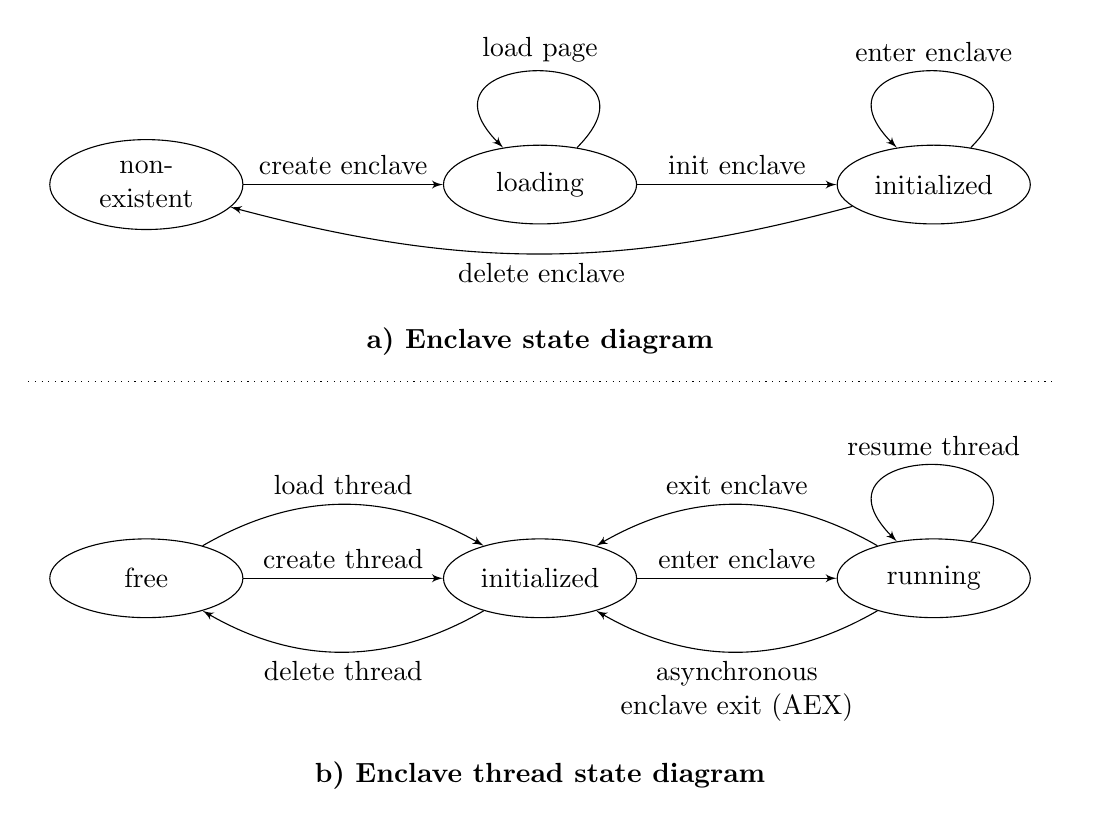
\begin{tikzpicture}[
	state/.style={draw, ellipse, text width=1.5cm, minimum height=1cm, align=center},
	arrow/.style={-latex'},
	heading/.style={font=\bfseries},
	label/.style={text width=3cm, align=center}
]
% enclave state
\node[heading] at (5,-2) {a) Enclave state diagram};

\node[state] (v1) at (0,0) {non-\\existent};
\node[state] (v2) at (5,0) {loading};
\node[state] (v3) at (10,0) {initialized};

\draw[arrow]  (v1) edge node[above, label] {create enclave} (v2);
\draw[arrow]  (v2) edge node[above, label] {init enclave} (v3);
\draw[arrow]  (v2) edge[loop, looseness=5] node[above, label] {load page} (v2);
\draw[arrow]  (v3) edge[loop, looseness=5] node[above, label] {enter enclave} (v3);
\draw[arrow]  (v3) edge[bend left=15] node[below, label] {delete enclave} (v1);

\node[state] (v1a) at (0,-5) {free};
\node[state] (v2a) at (5,-5) {initialized};
\node[state] (v3a) at (10,-5) {running};

% thread state
\node[heading] at (5,-7.5) {b) Enclave thread state diagram};

\draw[arrow]  (v1a) edge[bend left]  node[above, label] {load thread} (v2a);
\draw[arrow]  (v1a) edge             node[above, label] {create thread} (v2a);
\draw[arrow]  (v2a) edge[bend left] node[below, label] {delete thread} (v1a);

\draw[arrow]  (v3a) edge[bend right]  node[above, label] {exit enclave} (v2a);
\draw[arrow]  (v2a) edge             node[above, label] {enter enclave} (v3a);
\draw[arrow]  (v3a) edge[bend left] node[below, label] {asynchronous enclave exit (AEX)} (v2a);

\draw[arrow]  (v3a) edge[loop, looseness=5] node[above, label] {resume thread} (v3a);

\draw[dotted]  (-1.5,-2.5) -- (11.5,-2.5);
\end{tikzpicture}
}\caption{\textbf{State diagrams for enclave and thread state in Sanctum.}\label{ID_1455628057}
The states and transitions are very similar to those in SGX since Sanctum's design was largely inspired by SGX.\label{ID_388325382}
Reprinted from \cite{Costan}.\label{ID_615159607}
\label{ID_486639489}\label{figure:sanctum-state}}
\end{figure}

\item[TrustZone Trusted Language Runtime (TLR)\cite{Santos2014}]\label{ID_1712498850}
implements a .NET runtime that is isolated in TrustZone's secure world. Security critical parts of an application can be extracted into ``trustlets'' (similar to enclaves in SGX) which are executed within the TLR.\label{ID_843781337}

Apart from TrustZone as hardware the TCB includes the TLR implementation. As with all solutions with a software TCB at level \textit{c} or broader, TLR is susceptible to privilege escalation if the TLR is compromised.\label{ID_456338807}

Though TrustZone could support trusted I/O, this feature is not available in the TLR, as it would require adding drivers to the TCB.\label{ID_813431600}
TLR does not provide attestation. A remote party cannot verify the state of trustlets and the runtime it is interacting with. Thus, TLR does not strictly match the definition of trusted computing used in this thesis. It is listed as its implementation is interesting and comparable to other solutions.\label{ID_1734052719}
\item[Oasis\cite{Owusu2013}]\label{ID_1097915963}
is comparable to SGX but avoids encrypting memory in DRAM.\label{ID_1149911880}
The concept hinges on using caches as RAM so that secrets never leave the CPU, e.g. are never stored on DRAM.\label{ID_479354751}
To this end, Oasis adds a set of CPU instructions to ``enable an isolated execution environment contained entirely on chip''.\label{ID_269399808}
As the authors themselves remark, Oasis is inferior to SGX in that it only supports applications of a very limited size.\label{ID_1544780564}
\item[Fides\cite{Strackx2012}]\label{ID_1573635887}
uses a ``small dynamic hypervisor to isolate [enclaves]'' from the rest of the system. The hypervisor separates two virtual machines (VMs): the legacy and secure VM, similar to TrustZone.\label{ID_99725932}
A minimal secure kernel isolates the different enclaves (called ``self protecting module (SPM)'') in the secure world.\label{ID_1045769233}

The software TCB includes the hypervisor and secure kernel.\label{ID_1212833812}
A TPM is used to attest the hypervisor and security kernel state.\label{ID_391511184}
The legacy kernel is excluded from the TCB. The ``running legacy kernel is pulled in the legacy VM, and memory access control of both VMs is configured''. This is possible using the dynamic TPM measurement features.\label{ID_1472841998}

Attestation and data sealing are only available on the basic TPM level, which is bound to the overall system state. This means the hypervisor and secure kernel can be attested, and data can be sealed to this state. This cannot be done for individual modules.\label{ID_577386957}
\item[TrustVisor\cite{McCune2010}]\label{ID_1338218613}
was developed by the authors of Flicker, with the goal of improving performance.\label{ID_1509697723}
It avoids slow TPM calls on the critical path by providing a virtual micro-TPM to each enclave (called ``piece of application logic (PAL)''). With this micro-TPM, each enclave can be attested and perform data sealing.\label{ID_448665960}

The micro-TPMs are hosted by a trusted hypervisor, which is dynamically loaded and measured (as done by Fides).\label{ID_488141781}
Thus the software TCB includes the hypervisor. The chain of trust when validating an enclave attestation is rooted in the TPM measurement. The chain thus includes the enclave, the micro-TPM and the hypervisor.\label{ID_1898494666}

Unlike Fides, there is no secure kernel that isolates enclaves. This behaviour is emulated on a lower level by un-mapping enclave pages from the legacy operating system. Each enclave has its own virtual guest memory. \autoref{table:tc-comparison} shows the software TCB as \textit{d}, when really it only includes the hypervisor and enclave, but no operating system.\label{ID_708049480}
\item[Flicker\cite{McCune2008}]\label{ID_878060233}
enables fine-grained attestation and isolation of enclaves using only the dynamic attestation feature of a TPM and a supported CPU.\label{ID_445599816}

The intended use of the dynamic TPM measurement is to virtualise an untrusted operating system after booting it and lazily loading a privileged hypervisor (as described for Fides).\label{ID_1988839866}
To do so, the CPU enters a special execution mode to load the hypervisor with elevated privileges. During this time the legacy operating system is suspended. Its privileges are demoted to VM guest privileges. This way the untrusted operating system is effectively removed from the TCB.\label{ID_670518178}

Instead of loading a hypervisor Flicker executes the enclave during this special loading phase, which is called a ``Flicker session''.\label{ID_827948010}
This session is also measured. After a cleanup phase (e.g. caches) regular execution is resumed and the result is returned.\label{ID_1543044077}

This approach is nearly feature complete with regards to \autoref{table:tc-comparison}. It isolates enclaves on the same level as SGX. The hardware TCB only includes the TPM. The software TCB includes the enclave and only a small additional wrapper for handling parameter input/output and cleanup.\label{ID_504952060}

The main drawback of the approach is the performance. Slow TPM operations are on the critical execution path -- they are executed every time the enclave is executed.\label{ID_2022441}
Only one core is used and interrupts are disabled in the special CPU state. Thus the system is stalled for the duration of a Flicker session. For use in interactive systems, Flicker enclaves need to exhibit a very small runtime. This is diametrically opposed to TPM overhead incurred with each session.\label{ID_1920950472}
Only one Flicker session can be executed at any given point in time, as the special CPU mode is not intended for parallel use.\label{ID_466004716}

In summary, despite the apparent features and small TCB, Flicker is not well-suited for general-purpose applications due to its performance limitations.\label{ID_1094537554}
\end{description}\label{ID_294304177}
\subsection{Application Isolation\label{ID_94612974}\label{section:tc-apps}}
\begin{description}\label{ID_82011801}
\item[Microsoft Haven\cite{Baumann2014}]\label{ID_353301403}
uses SGX to isolate an entire legacy application within an enclave.\label{ID_97042978}
Along with the application, a library operating system (Drawbridge LibOS\footnote{\url{https://www.microsoft.com/en-us/research/project/drawbridge/}}) is included in the enclave.\label{ID_1807131257}
``Drawbridge LibOS is a version of Windows 8 refactored to run as a set of libraries within the picoprocess.''\footnote{A picoprocess can interact with the operating system only through a very narrow system call interface. This is similar to the system call interface that hardware VMs use.}\label{ID_465258009}

An additional shield module within the enclave mediates between the library operating system and the outside world (untrusted runtime).\label{ID_1475060210}
Any system call by the application is passed through the library operating system, secured by the shield module, and only then passed on through the untrusted runtime on to the untrusted operating system. The layers are depicted in \autoref{figure:haven}.\label{ID_1924838776}
This approach is re-visited in \autoref{section:sgx-hardening} in the context of SCONE.\cite[]{Arnautov2016}\label{ID_1989885067}
\begin{figure}[htbp]
\makebox[\textwidth][c]{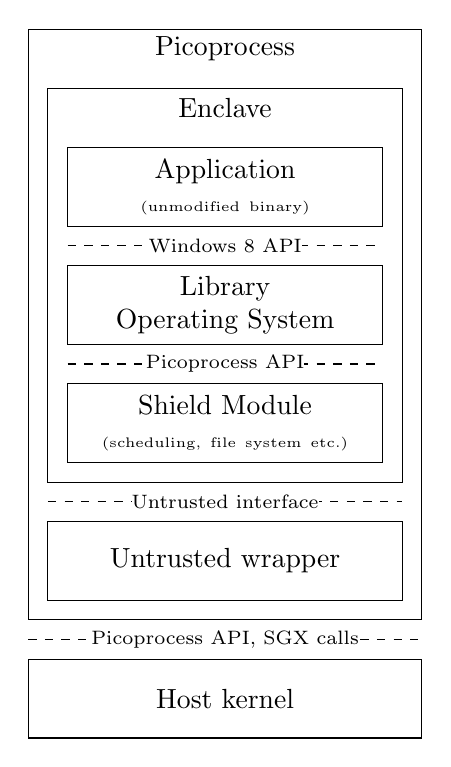
\begin{tikzpicture}[
    x=1cm,y=1cm,
	block/.style={draw, text width=4cm, minimum height=1cm, align=center, inner sep=0},
	label/.style={midway, font=\scriptsize, fill=white, inner sep=0}
]

\node[block] at (0,0) {Application\\\tiny(unmodified binary)};
\draw[dashed]  (-2,-0.75) -- (2,-0.75) node [label] {Windows 8 API};
\node[block] at (0,-1.5) {Library\\Operating System};
\draw[dashed]  (-2,-2.25) -- (2,-2.25) node [label] {Picoprocess API};
\node[block] at (0,-3) {Shield Module\\\tiny(scheduling, file system etc.)};

\node at (0,1) {Enclave};
\draw  (-2.25,1.25) rectangle (2.25,-3.75);
\draw[dashed]  (-2.25,-4) -- (2.25,-4) node [label] {Untrusted interface};
\node[block, text width=4.5cm] at (0,-4.75) {Untrusted wrapper};

\node at (0,1.75) {Picoprocess};
\draw  (-2.5,2) rectangle (2.5,-5.5);
\draw[dashed]  (-2.5,-5.75) -- (2.5,-5.75) node [label] {Picoprocess API, SGX calls};

\node[block, text width=5cm] at (0,-6.5) {Host kernel};
\end{tikzpicture}
}\caption{\textbf{Architecture of Microsoft Haven.}\label{ID_186584288}
The enclave (shaded green) isolates the entire unmodified application as well as a library operating system.\label{ID_1502290495}
Together with the shield module this protects the application from attacks by a malicious operating system.\label{ID_524857908}
The enclave interacts with the host kernel through a the narrow picoprocess API, as the library operating system abstracts from higher-level system calls.\label{ID_1865559949}
The untrusted wrapper only passes on calls from and to the enclave.\label{ID_1698784106}
Reprinted as a simplified version from \cite{Baumann2014}.\label{ID_1354023484}
\label{ID_1468585962}\label{figure:haven}}
\end{figure}


Haven re-purposes SGX in a fashion. SGX was designed to isolate small security-critical parts of an application inside individual enclaves.\label{ID_679922183}
This keeps the TCB small and can help when reasoning about security of the application.\label{ID_158610913}
Haven tries to find a different solution to secure unmodified legacy applications.\label{ID_1158551044}

This dramatically increases the size of the TCB but also provides additional benefits.\label{ID_967837581}
The application must not be refactored or modified.\label{ID_40595564}
In addition it protects against so-called Iago attacks by the operating system. A Iago attacks exploits the fact that an application may rely on a system call to be correctly executed instead of validating the results.\label{ID_810626140}

Haven is dated to 2014 and requires SGX, which is dated to 2015. Haven was implemented using SGX simulations and pre-release hardware before SGX-enabled CPUs became generally available.\label{ID_775639108}
\item[Minibox\cite{Li2014}]\label{ID_1759565280}
is comparable to TrustVisor, as it multiplexes the TPM into several virtual micro-TPMs.\label{ID_708706069}
Minibox has a slightly different focus, as it aims to be a ``two-way sandbox''.\label{ID_1073668755}
Traditional sandboxing protects the execution environment, e.g. the operating system, from malicious applications.\label{ID_1512132230}
Minibox protects both the operating system and the application.\label{ID_686729196}
Minibox executes applications in an isolated environment, called ``Mutually Isolated Execution Environment (MIEE)''.\label{ID_1462001648}

A hypervisor provides isolation and the micro-TPMs. It is included in the TCB.\label{ID_44939342}
The micro-TPMs enable data sealing and attestation on a per-application basis.\label{ID_1229123325}
A shield module in between checks and sanitises interaction in both directions.\label{ID_71322980}
\item[InkTag\cite{Hofmann2013}]\label{ID_1193381543}
isolates applications in the same way as many other solutions in this section: through virtualisation. This is similar to Windows IUM.\label{ID_330168128}
A hypervisor isolates the application, called ``high-assurance process (HAP)'', from the operating system.\label{ID_751005955}
The hypervisor provides ``secure files'', which can be seen as a form of data sealing.\label{ID_1357961035}

InkTag does not provide attestation, so a remote user cannot verify the state of the system.\label{ID_705281429}
With regards to the definition used in this thesis, it is therefor not strictly a trusted computing solution. Technically, it is interesting and comparable to other solutions and thus listed.\label{ID_643772456}

A distinguishing feature of InkTag is its ``para-verification''. The InkTag hypervisor verifies the behaviour of the operating system. HAPs can check the verification status using hypercalls.\label{ID_192984381}
To keep verification simple, InkTag requires the untrusted operating system to assist the hypervisor in its own verification.\label{ID_1553347413}

Another interesting aspect is how isolation is technically achieved.\label{ID_152315504}
InkTag does not rely on memory address translation as a hardware feature alone to isolate an HAPs memory.\label{ID_1866963112}
Instead, the hypervisor encrypts and hashes a HAPs memory pages on a context switch back to the operating system. This is somewhat comparable to SGX, where pages in DRAM are also encrypted.\label{ID_984786854}
To describe it in the author's words: ``InkTag uses hardware [memory management unit (MMU)] virtualisation for coarse-grained separation between secure and insecure data. Then it uses software only when needed, to manage the userspace portions of HAP page tables.''\label{ID_1124935151}
\item[Overshadow\cite{Chen2008}]\label{ID_1400272883}
is comparable to InkTag. A hypervisor isolates applications. The implementation differs.\label{ID_869320852}
Overshadow uses the terms ``shadowing'' and ``cloaking''. Memory is dynamically encrypted (cloaked) by the hypervisor depending on the ``shadow context'' accessing it.\label{ID_1595335407}
Only a cloaked application can read its own memory in decrypted form.\label{ID_213890862}

The hypervisor intercepts some system calls instead of passing them on to the untrusted operating system, such as file input and output.\label{ID_827784046}
Files accessed by applications are memory-mapped. With the cloaking mechanism in place they are thus automatically encrypted when written to disk.\label{ID_94227936}

The idea of transparently encrypting file input/output is similar to Haven, where unmodified applications are protected.\label{ID_1071753091}
Overshadow also tries to set a low adoption barrier by minimising necessary changes to legacy applications.\label{ID_5677792}

The hypervisor has a single secret key which it uses for memory encryption. The key is also used to e.g. protect file meta data integrity when written to disk.\label{ID_829303655}
This is somewhat similar to the memory integrity protection performed by SGX.\label{ID_1477727792}
However, SGX derives a unique key for every enclave (or enclave author).\label{ID_881038647}
The file encryption in Overshadow cannot be counted as data sealing, as the data is not sealed to a specific application but encrypted with the ``global'' hypervisor key.\label{ID_1562148172}

Like InkTag, Overshadow does not provide attestation and is, strictly speaking, not a trusted computing solution.\label{ID_436671458}
\end{description}\label{ID_1545531597}
\subsection{Operating System Isolation\label{ID_1279358890}}
\begin{description}\label{ID_1149112575}
\item[CloudVisor\cite{Zhang2011}]\label{ID_1588951554}
provides trusted VMs.\label{ID_1095393821}
VMs are an established deployment level in cloud environments.\label{ID_44643707}
Users typically trust the cloud provider to execute a VM properly and properly isolate it from other VMs. This trust is not technologically grounded.\label{ID_96896603}

CloudVisor provides trusted VMs based on two factors.\label{ID_661635791}
Firstly, VMs are protected from the hypervisor. This is implemented through nested virtualisation. A small security hypervisor in host mode controls the actual hypervisor.\label{ID_514198549}
The security hypervisor is comparably small. It is dynamically loaded and attested through the TPM. It thus does not contain boot loader code. This reduces the size of the TCB.\label{ID_926319613}
Secondly, the state of the security hypervisor can be remotely attested. A TPM is used for this. A user can then choose to release a VM image decryption key only to an attested hypervisor.\label{ID_175981473}

As for all trusted computing solutions that isolate on the virtualisation layer, the attack surface is large. If the guest operating system in a VM is compromised, all sensitive applications in that VM are compromised. Privilege escalation is also an issue.\label{ID_1893397931}
Also, CloudVisor does not protect against hardware attacks. Any party with hardware access can read the non-encrypted memory from DRAM (by tapping into the memory bus).\label{ID_791021042}

CloudVisor transparently inputs disk input/output.\label{ID_1740019798}
The data is not sealed to the VM state, but encrypted with a user-defined key.\label{ID_203575878}
Only the hypervisor state can be attested, not the state of an individual VM.\label{ID_1959689941}
\item[Nova\cite{Steinberg2010}]\label{ID_61001884}
is a micro-hypervisor, implemented from scratch.\label{ID_1979954588}
Using the same design principals as for micro-kernels, the Nova hypervisor is highly modularised.\label{ID_1097579055}
Its design follows the principle of least privilege.\label{ID_786963966}
Only the bare minimum of Nova runs at the super-privileged VMM kernel level.\label{ID_844682668}

Nova is not a trusted computing solution. However, it showcases the principle of least privilege. This should be kept in mind when developing applications from Intel SGX.\label{ID_1949063731}
\item[NoHype\cite{Keller2010}]\label{ID_399891803}
provides virtualisation without a hypervisor.\label{ID_1982528190}
Instead, resources are statically allocated: Each VM is allocated one CPU core and a slice of memory.\label{ID_1103417020}
However, VM management must still take place.\label{ID_460072436}
NoHype uses a management VM to load, start and stop other VMs.\label{ID_1653231210}
During execution, no interaction with a hypervisor is necessary.\label{ID_78679497}

NoHype does not run on standard hardware. It requires additional hardware virtualisation features that no CPU currently offers.\label{ID_1042436161}
NoHype limits a guest VM to a single core. It can parallelise across VMs, but not within VMs.\label{ID_1868828851}

NoHype addresses VM isolation, but no further features such as data sealing or attestation. As attestation is not provided, NoHype is not a trusted computing solution as defined in this thesis. It is still listed due to its interesting approach.\label{ID_1659320949}
\item[vTPM\cite{Perez2006}]\label{ID_253555451}
provides a virtual TPM to each VM.\label{ID_771624481}
This TPM is designed to match the VM life cycle. It can be stored, loaded and migrated with its VM.\label{ID_330974310}
The VM attestation provided by a virtual TPM is a compound attestation. The virtual TPM attests the VM. The hardware TPM attests the hypervisor and boot process.\label{ID_1083096548}

TrustVisor and Minibox provide virtual TPMs at the module and application level. vTPM provides virtual TPMs at the VM level.\label{ID_202468909}

An interesting aspect is how migration is enabled. The virtual TPMs have to be linked to the hardware TPM so that the process is rooted in a hardware root of trust.\label{ID_555144421}
If implemented naively, this would preempt the ability to later on migrate a virtual TPM to a different machine with a different hardware TPM.\label{ID_1205234476}
vTPM solves this using migrate-able TPM storage keys, which the TPM standard defines.\label{ID_964255737}
\item[Terra\cite{Garfinkel2003}]\label{ID_931924935}
is the first hypervisor-based solution for trusted computing.\label{ID_1552017657}
It introduced the idea of using a trusted hypervisor to isolate individual VMs.\label{ID_744934551}
In its design, Terra -- like vTPM -- uses a hardware device for data sealing and attestation.\label{ID_1233067999}
It then exposes these features to every VM.\label{ID_570557425}
The Terra prototype does not actually include such a hardware device. The authors identify a TPM as a good candidate.\label{ID_1769638002}
\end{description}\label{ID_1381661910}

\section{Comparison\label{ID_995120664}}
\autoref{table:tc-comparison} shows a comparison of all trusted computing solutions presented so far.\label{ID_31031823}
The table groups solutions by the TEE level they expose. Solutions with TEE level \textit{a} allow the developer to isolate separate modules of his application.\label{ID_1205678557}
The narrower the TEE level of isolation is, the smaller the isolated parts can be. This makes them easier to verify and less likely to contain security bugs.\label{ID_1993411071}

\begin{table}
\centering
\begin{threeparttable}
% exported from LibreOffice using Calc2Latex extension macro
\begin{tabular}{lcllllllccc}

\toprule
\multicolumn{3}{c}{\textbf{General}}                &   & \multicolumn{3}{c}{\textbf{Classification}}                                       &   & \multicolumn{3}{c}{\textbf{Features}}                     \\
\cmidrule(lr){1-3}                                      \cmidrule(lr){5-7}                                                                      \cmidrule(lr){9-11}
\textbf{Name}   & \h{Reference}         & \h{Year}  &   & \h{TEE Level\tnote{a}}    & \h{Software TCB\tnote{b}} & \h{Hardware TCB\tnote{c}} &   & \h{Attestation}   & \h{Data Sealing}  & \h{Parallelism}   \\ \midrule
Sanctum         & \cite{Costan}         & 2015      &   & a                         & a                         & custom CPU                &   & \cmark            &                   & \cmark            \\ 
Intel SGX       & \cite{McKeen2013}     & 2015      &   & a                         & a                         & SGX                       &   & \cmark            & \cmark            & \cmark            \\ 
TLR             & \cite{Santos2014}     & 2014      &   & a                         & c                         & TrustZone                 &   &                   & \cmark            & \cmark            \\ 
Oasis           & \cite{Owusu2013}      & 2013      &   & a                         & a                         & custom CPU                &   & \cmark            & \cmark            & \cmark            \\ 
Fides           & \cite{Strackx2012}    & 2012      &   & a                         & d                         & TPM, Virt.                &   & (\cmark)          &                   & \cmark            \\ 
TrustVisor      & \cite{McCune2010}     & 2010      &   & a                         & (d)                       & TPM, Virt.                &   & \cmark            & \cmark            & \cmark            \\ 
Flicker         & \cite{McCune2008}     & 2008      &   & a                         & a                         & TPM                       &   & \cmark            & \cmark            &                   \\ \midrule
Windows IUM     &                       & 2016      &   & b                         & d                         & Virt.                     &   &                   &                   & \cmark            \\ 
Haven           & \cite{Baumann2014}    & 2014      &   & b                         & c                         & SGX                       &   & \cmark            & \cmark            & \cmark            \\ 
MiniBox         & \cite{Li2014}         & 2014      &   & b                         & d                         & TPM, Virt.                &   & \cmark            & \cmark            & \cmark            \\ 
InkTag          & \cite{Hofmann2013}    & 2013      &   & b                         & d                         & Virt.                     &   & (\cmark)          & \cmark            & \cmark            \\ 
Overshadow      & \cite{Chen2008}       & 2008      &   & b                         & d                         &                           &   &                   &                   & \cmark            \\ \midrule
CloudVisor      & \cite{Zhang2011}      & 2011      &   & c                         & d                         & TPM, Virt.                &   & (\cmark)          &                   & \cmark            \\ 
Nova            & \cite{Steinberg2010}  & 2010      &   & c                         & d                         & Virt.                     &   &                   &                   & \cmark            \\ 
NoHype          & \cite{Keller2010}     & 2010      &   & c                         & c                         & custom CPU                &   &                   &                   & (\cmark)          \\ 
vTPM            & \cite{Perez2006}      & 2006      &   & c                         & d                         & TPM, Virt.                &   & \cmark            & \cmark            & \cmark            \\ 
Terra           & \cite{Garfinkel2003}  & 2003      &   & c                         & d                         & TPM, Virt.                &   & \cmark            & \cmark            & \cmark            \\ 
ARM TrustZone   & \cite{trustzone}      & 2003      &   & c                         & c                         & TrustZone                 &   &                   &                   & \cmark            \\ \midrule
TPM             & \cite{tcg:tpm2-arch}  & 2002      &   & d, e                      & d, e                      & TPM                       &   & \cmark            & \cmark            & \cmark            \\ 

\bottomrule
\end{tabular}
\caption{
\textbf{Comparison of trusted computing solutions.}\label{ID_1431047162}
Rows are ordered first by \textit{Trusted Execution (TEE) Level}, then by \textit{Year}. The columns \textit{TEE Level} and \textit{Software Trusted Computing Base (TCB)} refer to \autoref{figure:tee-granularity}.\label{ID_1895412115}
All commercial solutions can be used stand-alone (shown in their own row). Most commercial solutions are also used as hardware foundation by solutions from research (shown in the \textit{Hardware TCB} column).\label{ID_1108934633}
Solutions that do not support attestation cannot strictly be considered implementations of trusted computing. They do not support the verification step in \autoref{figure:trusted-computing}.\label{ID_946982666}
}
\label{table:tc-comparison}\label{ID_925340590}
\begin{tablenotes}\label{ID_1070677592}
\item[a] The software levels a developer must provide to use the solution. E.g. \textit{c} means that an operating system and the application must be provided. This value of this column is automatically the lower bound for the value of \textit{Software TCB}.\label{ID_429242638}
\item[b] The software levels that are included in the solution's TCB. E.g. \textit{d} means the entire virtualisation stack is included in the TCB. The software TCB is the union of software levels that the solution internally adds and the software levels the developer must add (\textit{TEE Level}).\label{ID_1226934143}
\item[c] \textit{Virt.} stands for hardware virtualisation support. \textit{SGX, TrustZone, TPM} refer to the respective commercial solutions.\label{ID_1945080258}
\end{tablenotes}\label{ID_1977590267}
\end{threeparttable}
\end{table}
The TEE level controls the flexibility and ease of adoption.\label{ID_1265116413}
A broader TEE level may be more insecure, but can facilitate re-use of unmodified VMs or applications.\label{ID_726502290}
Potentially, solutions higher up in the table can also emulate broader TEE levels.\label{ID_409119986}
Haven shows how SGX, which isolates at module level, can be used to isolate an entire application including a library operating system.\label{ID_1577048947}

Most solutions expose a narrow TEE level at the cost of a larger software TCB. TLR includes the secure kernel and .NET language runtime. Fides and TrustVisor include a hypervisor.\label{ID_289926468}
Such a large software TCB is required when the underlying hardware does not support isolation at the desired level. Solutions with a smaller software TCB require specialised hardware. This usually means a larger hardware TCB.\label{ID_7381152}
Shifting the TCB from software into hardware is not necessarily an improvement. Firstly, it is hard to draw a clear line between the two. SGX is considered a hardware feature, but is implemented mostly in micro-code, the firmware of the CPU.\cite[]{sgx-explained}\label{ID_135747553}
Secondly, a hardware implementation must not automatically be more secure than the alternative in software.\label{ID_1373303945}

All presented solutions utilise the CPUs processing power. A TPM is used as an external secure element by some. This is only responsible for attestation and handling of cryptographic keys.\label{ID_1726004639}
Some solutions such as Flicker and NoHype do not make full use of the CPUs processing power.\label{ID_1646772907}

This is to the author's knowledge the first comparison of its kind.\label{ID_122305244}
A comparison of security features of some solutions is presented in \cite{sgx-explained}.\label{ID_842412303}

\chapter{Intel SGX\label{ID_1888222908}\label{chapter:sgx}}
This chapter describes Intel Software Guard Extensions (SGX) in more detail. Costan et al. provide an exhaustive, in-depth description and analysis of SGX which is referred to as additional reading material.\cite[]{sgx-explained}\label{ID_870693712}
This chapter briefly describes the basic concepts of SGX and then summarises further findings from research.\label{ID_147500482}
This includes performance studies, known criticism and security issues, as well as noteworthy applications built on top of SGX.\label{ID_1316984123}
\begin{figure}[htbp]
\makebox[\textwidth][c]{\begin{tikzpicture}[
	block/.style={text width=3.5cm, draw, align=center, minimum height=0.5cm},
	gray/.style={color=gray},
	description/.style={font=\small}
]

% non root
\node[block] at (0,-0.6) {Application};
\node[block, fill=greenbg] at (0,0.1) {SGX Enclave};
\node at (-3,-0.25) {Ring 3};
\draw  (-4,0.5) rectangle (2,-1.5) {};

\draw  (-4,-1) rectangle (2,-1.5);
\draw  (-4,-2) rectangle (2,-1.5);
\node[gray] at (-3,-1.25) {Ring 2};
\node[gray] at (-3,-1.75) {Ring 1};

\node[block] at (0,-2.5) {Operating System};
\draw  (-4,-2) rectangle (2,-3);
\node at (-3,-2.5) {Ring 0};

\node[left] at (-4.5,-1.25) {VMX non-root};
% root
\draw (-4,-3) rectangle (2,-3.5);
\draw (-4,-3.5) rectangle (2,-4);
\draw (-4,-4) rectangle (2,-4.5);
\node[gray] at (-3,-3.25) {Ring 3};
\node[gray] at (-3,-3.75) {Ring 2};
\node[gray] at (-3,-4.25) {Ring 1};

\node[block] at (0,-5) {Hypervisor};
\draw  (-4,-3) rectangle (2,-5.5);
\node at (-3,-5) {Ring 0};

\node[left] at (-4.5,-4.25) {VMX root};
\draw[dashed] (-7.5,-3) -- (3,-3);

% smm
\node at (-1,-5.75) {BIOS};
\draw  (-4,-5.5) rectangle (2,-6);
\node[left] at (-4.5,-5.75) {SMM};
\draw[dashed] (-7.5,-5.5) -- (3,-5.5);

% description
\node[description] at (3.5,-6) {more privileged};
\node[description] at (3.5,0.5) {less privileged};
\end{tikzpicture}
}\caption{\textbf{Intel SGX enclave within the privilege level hierarchy.}\label{ID_1009832582}
An Intel CPU typically has two privilege schemes.\label{ID_135134113}
Privilege rings are the oldest concept, of which nowadays only ring zero and three are used to separate the operating system and applications. These are often called kernel and user mode.\label{ID_1292196585}
Virtualisation support adds another privilege scheme. The hypervisor runs in VMX root mode. It is protected from the guest VMs running in VMX non-root mode. The BIOS runs at the highest privilege level in system management mode (SMM).\label{ID_394725974}
SGX enclave mode adds an inverse isolation layer. The two existing privilege schemes protect more privileged components (bottom) from less privileged ones (top). SGX enclaves are in the least privileged layer, but are protected from all more privileged components.\label{ID_1068699047}
Reprinted from \cite{sgx-explained}.\label{ID_807064713}
\label{ID_1516228733}\label{figure:sgx-privilege}}
\end{figure}


\section{Overview\label{ID_1052911477}}
Intel SGX is a trusted computing solution. It is fully contained within the CPU and is exposed as an instruction set.\label{ID_1548132428}
As described in \autoref{chapter:tc-solutions}, SGX protects individual software modules in so-called ``enclaves''.\label{ID_884480539}
Compared to other solutions, the TCB is small. It includes only the protected module and the CPU.\footnote{The TCB also includes Intel's architectural enclaves.}\label{ID_1231030834}
SGX allows remote parties to verify the state of an enclave (attestation). It provides additional features, such as data sealing, on top.\label{ID_529967846}

The operating system, system management code and other parts of the application do not have to be trusted.\label{ID_1978585841}
The enclave is also protected from code running in system management mode (SMM), as well as from direct memory access (DMA).\cite[]{McKeen2013}\label{ID_508054107}
SGX changes the memory access semantics by introducing a protection scheme inverse to the existing privilege levels.\cite[ch. 6.2]{sgx-explained}. \autoref{figure:sgx-privilege} shows how enclaves relate to existing privilege levels.\label{ID_607406159}

\autoref{figure:sgx-address-space} shows an abstract view of an application's address space layout.\label{ID_1645584733}
The enclave's memory is protected by the CPU from direct access by any component but the enclave.\label{ID_1772616683}
When enclave memory is loaded into the CPU (caches), the CPU can enforce isolation by checking whether it is currently executing code of the correct enclave.\label{ID_1309432999}
If a memory page leaves the control of the CPU (when writing it to DRAM) it is encrypted and integrity-protected.\cite[]{Gueron}\label{ID_308074010}
More details on SGX's memory management are given in \autoref{section:sgx-perf}.\label{ID_879539859}
\begin{figure}[htbp]
\makebox[\textwidth][c]{\begin{tikzpicture}[
	block/.style={draw, text width=3.5cm, align=center, inner sep=0, minimum height=0.5cm}
]

\node[block, text width=4cm] at (-0.5,1.5) {Operating System};

\node at (-0.5,0.75) {Enclave};
\node[block] at (-0.5,0) {Entry Table};
\node[block] at (-0.5,-0.75) {Stack};
\node[block] at (-0.5,-1.5) {Heap};
\node[block] at (-0.5,-2.25) {Code};
\begin{scope}[on background layer]
\draw[fill=greenbg]  (-2.5,1) rectangle (1.5,-2.75);
\end{scope}

\node[block, text width=4cm] at (-0.5,-3.25) {App Stack};
\node[block, text width=4cm] at (-0.5,-4) {App Heap};
\node[block, text width=4cm] at (-0.5,-4.75) {App Code};
\end{tikzpicture}
}\caption{\textbf{Application address space with an Intel SGX enclave.}\label{ID_1596894882}
The CPU only allows access to the enclave's memory if it is currently executing code belonging to that very same enclave.\label{ID_811510196}
An enclave can be entered only at specific points in the code, defined in the entry table.\label{ID_1407494566}
The entire enclave memory (including code and entry table) is measured when the enclave is initialised. The CPU can attest to a remote party that it loaded the enclave correctly.\label{ID_1200889569}
Reprinted from \cite{McKeen2013}.\label{ID_1311428979}
\label{ID_1518668474}\label{figure:sgx-address-space}}
\end{figure}


An interesting aspect of SGX is that it relies on the untrusted operating system to perform its regular management tasks such as scheduling and memory allocation.\label{ID_96634994}
This includes the steps for setting up an enclave.\label{ID_307359552}
Enclave attestation would expose any attempts by a malicious operating system to load a tainted enclave.\label{ID_483221956}
Costan et al. put it like this: ``SGX design expects the system software to allocate the EPC pages to enclaves. However, as the system software is not trusted, SGX processors check the correctness of the system software’s allocation decisions.'' \cite[]{sgx-explained}\label{ID_729915388}
\autoref{figure:sgx-enclave-life-cycle} shows the enclave life cycle.\label{ID_1080928863}
\begin{figure}[htbp]
\makebox[\textwidth][c]{\begin{tikzpicture}[
	state/.style={draw, ellipse, text width=2cm, minimum height=1.4cm, align=center},
	arrow/.style={-latex'},
	label/.style={text width=3cm, align=center, font=\small}
]
\node[state] (v1) at (0,0) {non-\\existent};
\node[state] (v2) at (5,0) {unitialized};
\node[state, fill=greenbg] (v3) at (5,-3) {initialized\\(not in use)};
\node[state, fill=greenbg] (v4) at (0,-3) {initialized\\(in use)};

\draw[arrow]  (v1) edge node[above, label] {ECREATE} (v2);
\draw[arrow]  (v2) edge node[right, label, align=left] {EINIT} (v3);
\draw[arrow]  (v2) edge[loop, looseness=5, in=330, out=30] node[right, label, align=left] {EADD\\EEXTEND} (v2);
\draw[arrow]  (v3) edge[loop, looseness=5, in=300, out=240] node[below, label] {page management instructions} (v3);
\draw[arrow]  (v3) edge[bend left=15] node[below, label] {EENTER\\ERESUME} (v4);
\draw[arrow]  (v4) edge[bend left=15] node[above, label] {EEXIT\\AEX} (v3);
\draw[arrow]  (v3) edge[bend right=15] node[below left, label, align=right, pos=0.7] {EREMOVE} (v1);
\draw[arrow]  (v4) edge[loop, looseness=5, in=300, out=240] node[below, label] {page management instructions} (v4);
\draw[arrow]  (v4) edge[loop, looseness=5, in=210, out=150] node[left, align=right] {EGETKEY\\EREPORT} (v4);
\end{tikzpicture}
}\caption{\textbf{Intel SGX enclave life cycle.}\label{ID_1610889698}
The enclave's memory is protected in states shaded green.\label{ID_1686831062}
State transitions occur when CPU instructions are executed. E.g. \textit{ECREATE} creates a new, uninitialised enclave.\label{ID_805562591}
The operating system is expected to load the enclave by adding pages and extending the measurement of the enclave (similar to TPM measurement in \autoref{figure:tpm-measurement}).\label{ID_244657479}
Once \textit{EINIT} is called, the enclave is locked down. Its measurement is final and does not change when the enclave executes and changes internal data. The OS can no longer access the enclave's memory pages.\label{ID_1399476685}
The enclave can now only be entered via \textit{EENTER} (and after interrupts through \textit{ERESUME}) at locations defined in the entry table.\label{ID_98268923}
\textit{EGETKEY} and \textit{EGETREPORT} use the initial measurement (the enclave's \textit{identity}) for attestation and to derive cryptographic keys data sealing.\label{ID_1969992855}
The \textit{page management instructions} refer to paging into and out of Enclave Page Cache (EPC), a special memory area.\label{ID_1496257738}
Reprinted as a simplified version from \cite{sgx-explained}.\label{ID_1060342788}
\label{ID_538890645}\label{figure:sgx-enclave-life-cycle}}
\end{figure}

This reliance on the untrusted operating system keeps the SGX implementation small. It does however open up certain attack avenues. A denial of service (DoS) attack is straight-forward, as the operating system can refuse to schedule any enclave threads. In the context of remote computation, the infrastructure owner could choose to cut the power at any time, so this is not really a disadvantage.\label{ID_1767974666}
More serious security issues are described in \autoref{section:sgx-criticism}.\label{ID_1234909125}

Each SGX-capable CPU has an embedded cryptographic private key.\label{ID_85719808}
Using a special group signature scheme, the CPU uses this key to attest the state of an enclave.\cite[]{c}\label{ID_779581035}
Attestation can occur locally to setup secure communication channels between different enclaves on the same CPU.\cite[]{Anati2013}\label{ID_46728493}
It can also occur remotely. In this case, the attestation is not performed purely in hardware, but relies on additional so-called ``architectural enclaves''.\cite[]{sgx-explained}\label{ID_441975801}
These enclaves increase the size of the software TCB.\label{ID_1503953122}
They are also the main source for criticism of SGX as explained in \autoref{section:sgx-criticism}.\label{ID_419053144}

Code running in an enclave may not execute certain calls. These can only be handled by the untrusted wrapper.\cite[]{b}\label{ID_950941319}
Among them are instructions which may cause a \textit{VMEXIT}\footnote{CPUID, GETSEC, RDPMC, RDTSC, RDTSCP, SGDT, SIDT, SLDT, STR, VMCALL, VMFUNC}, input/output instructions\footnote{IN, INS/INSB/INSW/INSD, OUT, OUTS/OUTSB/OUTSW/OUTSD} and instructions which require a change in privilege levels (e.g. system calls).\footnote{Far call, Far jump, Far ret, INT n/INTO, IRET, LDS/LES/LFS/LGS/LSS, MOV to DS/ES/SS/FS/GS, POP DS/ES/SS/FS/GS, SYSCALL, SYSENTER}\cite[]{sgx-dev}\label{ID_909354065}
It is still possible to securely communicate with enclaves using a key exchanged during the attestation process.\label{ID_798355081}
An enclave can use a key derived from its identity (initial measurement) to encrypt any data it wishes to expose to the untrusted world.\label{ID_971079488}

Multiple threads can be active at the same time in an enclave.\cite[]{McKeen2013}\label{ID_900329339}
The number of threads must be statically defined before the enclave is initialised. Also, the maximum enclave size must be fixed before initialising the enclave.\footnote{SGX version 2 allows a dynamic number of threads and dynamic memory size. No hardware is available at the time of writing.}\label{ID_1383514787}
SGX capable CPUs are available since the end of 2015.\footnote{\url{https://github.com/ayeks/SGX-hardware}}.\label{ID_1264019871}

\section{Enclave Development\label{ID_816398624}\label{section:sgx-usage}}
Intel offers a Software Development Kit (SDK) for authoring enclaves and integrating them into an application.\label{ID_137499231}
The SDK is available for both Windows\footnote{\url{https://software.intel.com/en-us/sgx-sdk}} and Linux\footnote{\url{https://github.com/01org/linux-sgx}, open source under the very liberal BSD license.}\label{ID_1174967909}
The SDK provides the following features:\cite{sgx-windows,sgx-dev}\label{ID_1326046724}
\begin{description}\label{ID_1382376973}
\item[C and C++:] These are the only programming languages supported by the SDK.\label{ID_983565268}
\item[Interface definition:] An enclave's interface is defined in the Enclave Definition Language (EDL). This is described in more detail later on.\label{ID_378071151}
\item[Debugging:] This is actually a SGX hardware feature. An enclave in debug mode is not protected by the CPU.\label{ID_362995137}
\item[Simulation mode:] In the absence of SGX hardware, the hardware is simulated for development purposes.\label{ID_72514973}
\item[Trusted library:] Helper functions for enclave development. This includes a subset of the standard C library (e.g. without file input/output), random number generation, cryptographic primitives, key exchange and data sealing.\label{ID_1393938905}
\item[Complete authoring chain:] Enclaves can be compiled and signed so that they could be loaded in production use. See \autoref{section:sgx-criticism} for the restrictions that apply.\label{ID_237639086}
\end{description}\label{ID_934385781}
An example EDL interface definition is shown in \autoref{listing:edl}.\label{ID_614448952}
It is divided into a trusted (E-call) and untrusted (O-call) section.\label{ID_1379790192}
Based on this interface, the SDK generates proxy functions. For all \textit{trusted} functions (E-calls) proxies are generated for the untrusted wrapper. For all \textit{untrusted} functions (O-calls), proxies are generated for the enclave.\label{ID_1582039127}

The proxy code is necessary for parameter marshalling.\label{ID_930140065}
The function signature includes additional annotations for the parameters.\label{ID_1680143487}
The annotations show the direction of data flow (\textit{in, out, user\_{}check}).\label{ID_1178777303}
If \textit{in} (and/or \textit{out}) are specified, the proxy code will copy the parameter by value before calling the function (and/or afterwards). A pass-by-reference can be achieved with \textit{user\_{}check}.\label{ID_77293385}
Pass-by-value is recommended for security reasons. The enclave cannot rely on untrusted memory to be stable. However, copying and checking parameters adds overhead. This is discussed in \autoref{section:sgx-perf}.\label{ID_1962499209}
% Listing
\lstinputlisting[label=listing:edl,caption={
\textbf{enclave.edl}\protect\footnote{ \url{https://github.com/ftes/sgx-lib-consumer/blob/thesis/enclave/enclave.edl}} -- Enclave Definition Language (EDL) example file.\label{ID_1712028152}
EDL is used by the Intel SGX SDK to specify an enclaves interface on the function level.\label{ID_689768123}
The enclave's entry table is generated based on the trusted section of the EDL file.\label{ID_1488600472}
This EDL file defines only E-calls, but no outgoing (untrusted) O-calls.\label{ID_1871393222}
The example is taken from the demo consumer of the author's SGX helper library.\label{ID_704042173}
},style=edl]{../sgx-lib-consumer/enclave/enclave.edl}

The proxy needs to know how much data to copy for pointer arguments. This is handled by the annotations \textit{size, sizefunc} and \textit{count}. The first two define the size of an individual element statically or dynamically. The number of elements can be defined with \textit{count} either statically as a number or dynamically by referencing a different scalar parameter.\label{ID_1101116303}
For a full reference of EDL, see \cite{sgx-windows}.\label{ID_294430690}

The \textbf{from \ldots import} in \autoref{listing:edl} also shows how EDL files can be composed. In this case, library helper functions are included.\label{ID_1465748199}
This is also the method of choice for adding remote attestation and key exchange to an enclave.\footnote{\url{https://github.com/01org/linux-sgx/blob/1115c195cd60d5ab2b80c12d07e21663e5aa8030/SampleCode/RemoteAttestation/isv_enclave/isv_enclave.edl}}\label{ID_1804743643}
The helper library in question assists in prototyping SGX enclaves and is described in \autoref{chapter:sgx-lib}.\label{ID_597042526}

In addition to the architectural enclaves (attestation etc.), Intel also provides some helper enclaves as part of the Platform Software (PSW).\label{ID_1056979156}
These enclaves expose functionality such as monotonic counters and trusted time.\cite[]{sgx-windows}\label{ID_1018912990}
They can be accessed via trusted library functions included in the SDK.\label{ID_296716001}
These enclaves rely on the Manageability Engine (ME), which is a part of Intel CPUs, to provide these features.\footnote{\url{https://software.intel.com/en-us/forums/intel-software-guard-extensions-intel-sgx/topic/607330 }}\label{ID_1422515691}

\section{Performance\label{ID_388809349}\label{section:sgx-perf}}
In principle, the CPU's full processing speed is available in SGX enclaves. This is an advantage over solutions with external secure elements.\label{ID_1639328080}
However, several factors have a observable performance impact on enclave performance.\label{ID_935750308}
Isolation is achieved by protecting an enclave's memory.\label{ID_88365959}
The additional memory layers introduced to enforce this isolation have an impact on access speed.\label{ID_921734519}
Using Intel's SDK on the other hand apparently results in a larger performance impact.\label{ID_589701637}
Existing findings from research are now presented.\label{ID_1990153751}

\autoref{figure:sgx-memory-access-speed} shows what performance overhead an enclave has on memory access.\label{ID_1704912531}
Pre-fetching hides most of the performance impact for sequential reads and writes.\cite[]{Arnautov2016}\label{ID_1962030152}
Random reads and writes highlight the actual performance impact.\label{ID_1830401881}
Two major factors impacting access times can be identified in the diagram.\footnote{\cite{sgx-dev} also lists these as performance bottlenecks.}\cite[]{Arnautov2016}\label{ID_334642516}
\begin{description}\label{ID_1147500560}
\item[L3 cache size:] Enclave memory remains decrypted within the CPU's caches. As long as all enclave memory fits in the L3 cache, memory access times are roughly equal. If the cache is exceed, pages must be fetched from DRAM, decrypted and integrity-checked.\label{ID_635553127}
\item[Enclave Page Cache (EPC) size:] The EPC is a special section of DRAM. Pages that do not fit into EPC must be paged out to regular sections of DRAM. The EPC size is limited to 128MB on current SGX CPUs, of which 92MB can be used by user's enclaves. The rest is needed for meta data and Intel's architectural enclaves.\label{ID_766702921}
\end{description}\label{ID_1904020196}
\begin{figure}[htbp]
\makebox[\textwidth][c]{
	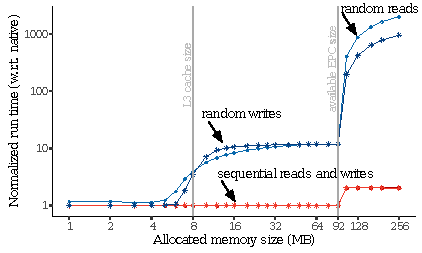
\includegraphics[width=0.8\textwidth]{content/images/sgx memory access speed}
}\caption{\textbf{Memory access speed in Intel SGX enclaves.} Access times are normalised w.r.t native (non-enclave) access. The two limiting factors, L3 cache size and Enclave Page Cache (EPC) size are shown as grey lines. Sequential access hides some of the overhead due to pre-fetching. Reprinted from \cite{Arnautov2016}.\label{ID_1423936467}\label{figure:sgx-memory-access-speed}\label{ID_1423936467}\label{figure:sgx-memory-access-speed}}
\end{figure}


This performance overhead means that enclave memory is a valuable resource and must be managed accordingly.\label{ID_813062369}
If possible, the combined size of all enclaves on a system should remain beneath the magical 92MB limit to avoid the 1000x performance penalty.\label{ID_1432243820}
Even better, the size of the L3 cache should not be exceeded.\label{ID_62762820}

The SDK provided by Intel should also be used with caution regarding performance. The SDK introduces the concept of E-calls and O-calls, which are synchronous transitions into and out of the enclave.\cite[]{b}\label{ID_1781049317}
The SDK's performance is evaluated in \cite{Arnautov2016}.\label{ID_905850038}
They compare different solutions for executing system calls from within an enclave.\label{ID_1493078645}
The first option is to use the untrusted wrapper as a synchronous proxy (E-call for every system call). The CPU must switch execution context, execute the system call, and pass the result back to the enclave. This adds a 10x overhead for file input/output.\label{ID_642315590}
Better performance is achieved with an asynchronous executor thread pool outside of the enclave. This solution results in performance comparable to native execution.\cite[]{Arnautov2016}\label{ID_1629826277}
However, the Intel SDK can apparently not be used to build this complex kind of interaction.\label{ID_501911684}

\section{Known Criticism\label{ID_806492894}\label{section:sgx-criticism}}
Intel SGX is a technically exciting solution for trusted computing.\label{ID_1751677516}
Related to SGX, criticism has been voiced on multiple levels.\label{ID_1329458344}
It ranges from critique of trusted computing in general, debatable SGX design decisions up to security bugs.\label{ID_49832717}
\begin{description}\label{ID_1676577849}
\item[Trusted computing in general:]\label{ID_1171380944}
The release of a commercially available solution for trusted computing has re-triggered an existing debate. Intel SGX protects enclaves from any access by the operating system and hardware owner.\label{ID_1042141723}

Depending on the standpoint this may be a desirable feature or an intrusion into personal rights.\label{ID_996020323}
When deploying an application to the cloud, it may be desirable for the software vendor to keep certain data secret from the infrastructure provider and other tenants.\label{ID_1818979325}
When developing a blu-ray player (see \autoref{section:sgx-apps}), it may be desirable for the blu-ray industry to keep decryption keys secret and guarantee that digital rights are not infringed.\label{ID_606336711}
When executing an application as an end user or infrastructure provider, it may be desirable to be in full control of the application.\label{ID_130834011}

SGX turns the tables: the software vendor can -- to a certain degree -- take control of the hardware without interference of the hardware owner.\label{ID_1498236698}
This gives cause to debates of ownership.\label{ID_290775852}
\item[Malware in enclaves:]\label{ID_1718158893}
Enclaves are protected from the operating system and hardware owner. This can also be a disadvantage from a security standpoint. Malware protected in an enclave is an often stated example.\label{ID_1912630411}
Two factors are in place that should prevent this.\label{ID_1621688747}
Firstly, enclaves cannot perform any input/output, so part of the malware would have to live in an (observable) unprotected wrapper.\cite[ch. 6.8]{sgx-explained}\label{ID_161645023}
Secondly, Intel can decide which enclave software will be loaded by an Intel CPU (white labelling). This is again a cause of criticism.\label{ID_351871068}

Intel only white labels the identity of an enclave -- its initial measurement. Because enclave code may be self-modifying it is possible to dynamically load encrypted malicious code into an enclave. This is a viable attack vector if an exploit is found for a white labelled enclave, into which malware could then be loaded.\cite[]{schwarz2017malware}\label{ID_1914733350}
AsyncShock is a tool that can help exploit enclave bugs. It targets synchronisation bugs in enclaves. Using such a bug AsyncShock helps to extract secrets or modify the control flow in that enclave. Enclaves approved by Intel could then be misused.\cite[]{Weichbrodt2016}\label{ID_1238669801}
\item[Side-channel attacks:]\label{ID_140344652}
The following attacks have been successfully identified. The first two have been successfully carried out.\label{ID_1298323933}
\begin{itemize}\label{ID_1098508864}
\item Memory access pattern analysis of well-known libraries in an enclave. This is done with the help of the operating system, which simulates page faults to detect memory access. As a result, images processed by a library within an enclave were re-constructed. Oblivious RAM techniques and address space layout randomisation are proposed as counter-measures.\cite[]{Xu2015}\label{ID_784348582}
\item Cache Prime+Probe attack on co-located enclaves. Based on knowledge of instruction execution times, the authors could measure memory access times from within an enclave and deduce cached values. With this technique an RSA key was extracted from another enclave running a standard RSA implementation. The authors propose several countermeasures. This attack highlights the problem of having protected malware inside an SGX enclave.\cite[]{schwarz2017malware}\label{ID_1818357587}
\item Hyper-threading execution timing. SGX does not prevent the use of hyper-threading. If an enclave shares a logical processor with a snooping thread that thread could find out what instructions the enclave is executing as well as its memory access patterns. The authors propose to disable hyper-threading. Also the hyper-threading status should be included in the enclave measurement so that it can be attested.\cite[]{sgx-explained}\label{ID_1173647836}
\end{itemize}\label{ID_960745123}
\begin{figure}[H]
	\begin{center}
	\begin{subfigure}[b]{0.4\textwidth}
		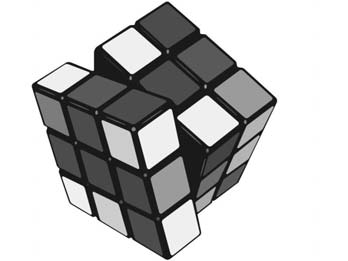
\includegraphics[width=\textwidth]{content/images/sgx page fault 1}
		\caption{original\label{ID_508330768}}
	\end{subfigure}
	\begin{subfigure}[b]{0.4\textwidth}
		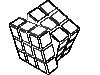
\includegraphics[width=\textwidth]{content/images/sgx page fault 2}
		\caption{recovered\label{ID_105623928}}
	\end{subfigure}
	\caption{\textbf{Result of a side-channel attack on SGX.} By analysing the memory access pattern of an enclave running the image processing library \textit{libjpeg}, certain features of the input image could be reconstructed. Reprinted from \cite{Xu2015}.\label{ID_172988213}}
	\end{center}
\end{figure}

\item[Vulnerability of architectural enclaves:]\label{ID_782196997}
SGX mainly consists of hardware: CPU microcode and memory encryption engine.\label{ID_1187633218}
To make it feature-complete and usable, Intel adds some architectural enclaves (launch enclave, quoting enclave) and platform software (PSW).\label{ID_306094396}
This keeps the hardware TCB small at the cost of a larger software TCB.\label{ID_119641221}
The quoting enclave access the CPU's attestation key.\label{ID_321415880}
A bug in the quoting enclave could expose that attestation key.\label{ID_1321164653}
Intel's EPID group signature scheme allows revocation of individual keys. But a quoting enclave bug would potentially expose the attestation keys of all SGX CPUs until a patched quoting enclave is deployed.\cite[]{c}\label{ID_1629332890}
Intel is thus under constant pressure to keep it's architectural enclaves secured against any new attacks.\label{ID_1159889792}
An exploit for an architectural enclave would also allow malware to be loaded into a protected enclave as described earlier.\label{ID_1914496271}
\item[Intel controls enclave launch:]\label{ID_27203074}
Enclave launching, like attestation, is also implemented in software in an architectural enclave.\label{ID_149498049}
This lets Intel control which enclaves may be launched.\label{ID_1496527821}
An enclave can be loaded either if it is authored by Intel (e.g. the launch enclave) or if the launch enclave grants the launch.\label{ID_1663962426}
Based on Intel's patents for SGX, Costan et al. surmise that ``the Launch Enclave is intended to be an enclave licensing mechanism that allows Intel to force itself as an intermediary in the distribution of all enclave software''.\cite[]{sgx-explained}\label{ID_520209509}

This allows Intel to prevent malicious software from being loaded.\label{ID_6860923}
This also allows Intel to control which software is loaded in general.\label{ID_1791148432}
The benefits for Intel from a business standpoint are obvious.\label{ID_1766310969}
This level of control over an end-users hardware can be seen as ``software security equivalent to the Net Neutrality debates''.\cite[]{sgx-explained}\label{ID_1069483865}
\end{description}\label{ID_1258675258}

\section{Applications\label{ID_54364136}\label{section:sgx-apps}}
Leaving the (well-founded) criticism behind, SGX has the potential to be the foundation for innovative applications.\label{ID_1994267622}
This section highlights some interesting SGX-based applications from research.\label{ID_492049202}
It does not describe such applications that themselves can be considered frameworks or infrastructure layers for securing other applications such as SCONE or Haven. These are discussed in \autoref{section:sgx-hardening}.\label{ID_110180016}
\begin{description}\label{ID_1142331261}
\item[Proof of elapsed time:]\label{ID_1448411725}
Bitcoin is the prototypical ledger-based crypto-currency.\label{ID_878352987}
Its security revolves around the notion of proof-of-work.\label{ID_1836284802}
As long as the assumption holds that the majority of processing power in the Bitcoin network belongs to honest users, the majority of the network eventually behaves as expected.\cite[]{nakamoto2008bitcoin}\label{ID_1051235374}

The proof-of-work to be brought forward in Bitcoin is the solution of a hash puzzle. Participants (miners) must hash a fixed input combined with an input of their choice so that the resulting hash satisfies a certain criteria.\label{ID_148196853}
The first miner to find a solution to the puzzle wins.\label{ID_203871180}
Competing in the network requires investment of processing power and thus money.\label{ID_8052086}

The downside is that this processing power is invested in finding a solution to a random puzzle. This solution has no inherent value outside of Bitcoin.\label{ID_331211373}
Alternative crypto-currencies such as Primecoin use puzzles with solutions that have an inherent value, such as finding new prime numbers.\cite[]{king2013primecoin}\label{ID_1916667021}

A different approach based on SGX enclaves is proposed in Intel's Sawtooth\footnote{\url{https://intelledger.github.io}} project.\label{ID_1210248514}
Sawtooth introduces proof-of-elapsed-time (PoET) as an alternative to proof-of-work.\label{ID_1984325994}
Essentially, Intel CPUs are used as an attestable source of true random numbers. If this number is viewed as a wait time, the participant to generate the lowest wait time wins.\cite[]{Intel}\label{ID_359563617}
\item[Digital rights management (DRM):]\label{ID_951757571}
The current version of Cyberlink's PowerDVD requires SGX hardware for playback of ultra high definition (UHD) blu-rays.\cite[]{powerdvd}\label{ID_1044376464}
This is an example of how SGX can be used on consumer devices rather than cloud infrastructure.\label{ID_1177830256}
Cyberlink does not explain what SGX is used for. It is likely that an enclave handles the decryption of the blu-rays content.\label{ID_1342908426}
The decryption key would then only provided to attested enclaves by the Cyberlink server.\label{ID_294479514}
\item[Secure ZooKeeper:]\label{ID_1198544376}
ZooKeeper\footnote{\url{https://zookeeper.apache.org/}} is a key-value store used to provide configuration, naming, synchronisation etc. in distributed applications (e.g. micro-service architectures).\label{ID_1070130646}
SGX can be used to harden existing applications, which is the topic of this thesis.\label{ID_277356659}
SecureKeeper uses enclaves to protect the data managed by ZooKeeper.\label{ID_1700491540}
When the data is stored outside of the enclave, e.g. on disk, it is encrypted.\label{ID_204377492}
The Java native interface (JNI) is used to bind the Java implementation of ZooKeeper to the enclaves.\cite[]{Brenner2016}\label{ID_808626981}
\item[Secure Hadoop map-reduce:]\label{ID_1200794013}
VC3 is a prototype of Microsoft Research that ``runs distributed MapReduce computations in the cloud while keeping their code and data secret.''\label{ID_1876953859}
Hadoop is used as the underlying map-reduce engine.\label{ID_956606489}
The map and reduce jobs run within enclaves.\label{ID_1313741719}
All other software components such as Hadoop or the operating system are kept outside of the TCB.\label{ID_1560260688}
Enclave code, input data and the results remain encrypted when outside of enclaves.\label{ID_1156084768}
VC3 achieves full Hadoop compatibility by performing all setup steps ``in-band'' as map-reduce jobs: distributing enclave code, performing attestation, and distributing data decryption keys.\cite[]{Schuster2015}\label{ID_322840088}
\end{description}\label{ID_1340304870}

\section{Conclusion\label{ID_95827774}}
SGX is the first trusted computing solution that is likely to see widespread adoption.\label{ID_1283663236}
It is shipped with many current Intel desktop processors\footnote{\url{https://github.com/ayeks/SGX-hardware}}.\label{ID_1220353350}
SGX has potential use-cases for both end-consumer devices and cloud infrastructure.\label{ID_1092135395}
Its main advantage when compared to other solutions is the achievable processing speed. SGX provides module-level TEEs and has an small overall TCB.\label{ID_744293523}

There are many potential security issues and weighty criticism regarding Intel's design decisions and the influence Intel thus has over end-user hardware.\label{ID_856863719}
Only time can tell how well SGX as a technology will be received and whether it can live up to its expectations.\label{ID_1859137509}
The continued security of the architectural enclaves seems to be a crucial factor.\label{ID_773096886}

\chapter{Intel SGX Helper Library\label{ID_985966487}\label{chapter:sgx-lib}}
The case studies conducted for this thesis use the Intel SGX SDK for Windows.\footnote{At implementation time (first half of 2016), the Linux SDK was not yet available.}\label{ID_1132198097}
To make prototyping faster and easier, a helper library wrapping the SDK was developed alongside the case studies.\label{ID_111937508}
The library contains scripts and wrapper functions that make working with the SDK easier.\label{ID_1184988902}
The library also assists in constructing a shim C library (\autoref{figure:scone-interface}).\label{ID_1179607118}
The concepts of this library and some usage guidelines are introduced in this chapter.\label{ID_553638787}

The full code is not printed in this chapter or the appendix. Please refer to the Git repository.\footnote{\url{https://github.com/ftes/sgx-lib/tree/thesis}}\label{ID_1903948230}
The repository also contains more in-depth details on configuration and usage.\label{ID_191350613}
A demo consumer project showcases usage of the library.\footnote{\url{https://github.com/ftes/sgx-lib-consumer/tree/thesis}}\label{ID_1523691323}
The Git tag \Q{thesis} in these repositories marks the commit from which the code listings in this thesis are taken.\label{ID_1811245411}

No SGX hardware was available at the time of implementation. The library is only usable for simulation mode. It can not be used in production-ready enclaves.\label{ID_1484453818}

The library is split into a trusted and untrusted module.\label{ID_1011030349}
The consumer can include the header files and link against these library modules.\label{ID_1462993309}
Also, the consumer must include the library's EDL file in his.\label{ID_1600152309}

The library tries to help with four aspects of enclave development:\label{ID_1627717648}
\begin{description}\label{ID_1696400236}
\item[Generate O-call proxies:]\label{ID_1577901159}
This is necessary if the C library lives outside of the enclave. Then a shim is needed inside the enclave to proxy calls to the outside (see \autoref{figure:scone-interface}).\label{ID_1843451651}
Defining these proxies involves touching several files and repeatedly inserting a similar method signature.\label{ID_1189822781}
The \Q{add_ocall.sh} script speeds up this process.\label{ID_1596596706}
See \autoref{table:sgx-lib} for details on how to use this script.\label{ID_1961827742}

As an example, consider adding a proxy for the \Q{_ftelli64}\footnote{\url{https://msdn.microsoft.com/de-de/library/0ys3hc0b.aspx}} Windows C library function.\label{ID_2348280}
The helper script has to be called as shown in \autoref{listing:add-ocall}.\label{ID_1088589749}
\lstinputlisting[label=listing:add-ocall,style=default,language=bash,caption={
\textbf{Example invocation of O-call generation script.} The script generates EDL code, trusted header code and trusted and untrusted proxy implementations.\label{ID_306321559}
The environment variables do not have to be set. Their default values correspond to the directory and file layout of the library.\label{ID_116451330}
}]{content/listings/add-ocall.txt}

The following listings show the code generated by the script. \autoref{figure:lib-proxies} shows how the generated code interacts with the SDK and C library.\label{ID_774243892}
\begin{figure}[htbp]
\makebox[\textwidth][c]{\begin{tikzpicture}[
	block/.style={draw, align=center, text width=5cm, minimum height=0.7cm, inner sep=0},
	arrow/.style={-latex'}
]

\node at (0,1.5) {Enclave};
\node[block] (v1) at (0,0.5) {Custom code};
\node[block] (v1b) at (0,-0.75) {Library-generated proxy};
\node[block] (v2) at (0,-2) {SDK-generated proxy};
\begin{scope}[on background layer]
	\draw [fill=greenbg] (-2.75,2) rectangle (2.75,-2.75);
\end{scope}

\node[block] (v3) at (0,-3.5) {SDK-generated proxy};
\node[block] (v4) at (0,-4.75) {Library-generated proxy};
\node[block] (v5) at (0,-6) {C Library};
\draw [arrow] (v1) edge (v1b);
\draw [arrow] (v1b) edge (v2);
\draw [arrow] (v2) edge (v3);
\draw [arrow] (v3) edge (v4);
\draw [arrow] (v4) edge (v5);
\end{tikzpicture}

}\caption{\textbf{Interaction of proxies generated by Intel's SDK and the helper library.}\label{ID_1914549896}
The SDK proxies deal with parameter handling. Depending on the EDL definition, parameters are checked and copied back and forth.\label{ID_331655439}
The enclave library proxy checks the return value and prints human readable error messages. The untrusted library proxy delegates to the C library.\label{ID_1047121255}
\label{ID_811027800}\label{figure:lib-proxies}}
\end{figure}

\lstinputlisting[label=listing:lib-edl,caption={
\textbf{sgx\_{}lib.edl (extract).}\protect\footnote{\url{https://github.com/ftes/sgx-lib/blob/thesis/sgx_lib_t/sgx_lib.edl}}\label{ID_1403293956}
The EDL interface definition is extended with the O-call.\label{ID_271766819}
This does not affect the enclave entry table, as this only controls the allowed E-calls.\label{ID_1356327165}
},firstnumber=46,linerange={46-47},style=cpp,autodedent]{../sgx-lib/sgx_lib_t/sgx_lib.edl}\label{ID_1536712624}
\lstinputlisting[label=listing:t-stdio,caption={
\textbf{sgx\_{}lib\_{}t\_{}stdio.h (extract).}\protect\footnote{\url{https://github.com/ftes/sgx-lib/blob/thesis/sgx_lib_t/include/sgx_lib_t_stdio.h}}\label{ID_188697395}
The trusted header file is modified to include the proxy function's signature.\label{ID_1928208466}
},firstnumber=41,linerange={41-42},style=cpp]{../sgx-lib/sgx_lib_t/include/sgx_lib_t_stdio.h}\label{ID_1829796801}
\lstinputlisting[label=listing:t-stdio-c2,caption={
\textbf{sgx\_{}lib\_{}t\_{}stdio.c (extract).}\protect\footnote{\url{https://github.com/ftes/sgx-lib/blob/thesis/sgx_lib_t/sgx_lib_t_stdio.c}}\label{ID_472958}
The trusted proxy implementation.\label{ID_1583369182}
The proxy also acts as an adapter. It converts the O-calls signature (with the return value passed as a pointer) to the original signature.\label{ID_1261394446}
The proxy checks for errors. If an error is encountered, a meaningful error description is printed using an O-call.\label{ID_1625059582}
},firstnumber=190,linerange={190-195},style=cpp]{../sgx-lib/sgx_lib_t/sgx_lib_t_stdio.c}\label{ID_986440387}
\lstinputlisting[label=listing:u-stdio-c,caption={
\textbf{sgx\_{}lib\_{}u\_{}stdio.c (extract).}\protect\footnote{\url{https://github.com/ftes/sgx-lib/blob/thesis/sgx_lib_u/sgx_lib_u_ocalls_stdio.c}}\label{ID_1550359463}
The untrusted proxy implementation. This simply delegates to the C library implementation.\label{ID_423213693}
},firstnumber=35,linerange={35-38},style=cpp]{../sgx-lib/sgx_lib_u/sgx_lib_u_ocalls_stdio.c}\label{ID_1509333371}

The untrusted wrapper seems superfluous. Rather, the SDK could directly be linked to the C library implementation.\label{ID_547328155}
The SDK supports this feature by adding \Q{[cdecl, dllimport]} to a function signature in the EDL file.\cite[]{sgx-windows}\label{ID_1497646761}
However, the generated stub in the enclave has a different signature in case the function has a return value. The generated signature of the trusted \Q{fopen} O-call is shown in \autoref{listing:ocall-fopen}.\label{ID_446408595}
\begin{lstlisting}[style=cpp, numbers=none, label=listing:ocall-fopen, caption={\textbf{Generated O-call signature for standard C library function.} The SDK passes the return value via a pointer parameter.}]
void fopen(FILE* retVal, const char* filename, const char* mode);
\end{lstlisting}
To use unmodified legacy code in an enclave, the library functions must have the exact same signature.\label{ID_1472270465}
To provide trusted functions with the original signature, one has to overload the functions in the enclave. This is not possible in C. The library is written in C to facilitate usage in both C and C++ projects.\label{ID_104777994}
As a workaround the O-calls are appended with a \Q{_ocall} suffix. No overloading is thus necessary. Instead, an untrusted proxy implementation is generated which delegates to the C library implementation.\label{ID_1394611332}
\item[Translate error codes to messages:]\label{ID_1725641591}
A variety of error codes is defined for SGX\footnote{\url{https://software.intel.com/en-us/node/709252}}.\label{ID_1308659811}
Many SDK functions and the generated proxies can return these error codes.\label{ID_383627344}
Manually looking up their meaning is time-consuming.\label{ID_1960603292}

The library contains a trusted\footnote{\url{https://github.com/ftes/sgx-lib/blob/thesis/sgx_lib_t/sgx_lib_t_util.c\#L10}} and untrusted\footnote{\url{https://github.com/ftes/sgx-lib/blob/thesis/sgx_lib_u/sgx_lib_u_util.c\#L8}} utility function to check the return value.\label{ID_104103671}
The descriptions are scraped from the Intel SDK's \Q{sgx_error.h}\footnote{The version included in the Windows SDK is probably identical to the Linux version: \url{https://github.com/01org/linux-sgx/blob/sgx_1.9/common/inc/sgx_error.h}} file.\label{ID_1860489535}
The scraping script is included as part of the library. It has to be re-executed in case the error codes or messages change. For usage details, see \autoref{table:sgx-lib}.\label{ID_163886822}
\item[Developer-friendly encryption:]\label{ID_1982795261}
The SDK includes a cryptography library.\label{ID_66289720}
It can also seal data to an enclave's identity (see \autoref{section:tc}).\label{ID_1914463209}
However, some of the SDK's cryptography functions are cumbersome to use.\label{ID_1318478695}
Due to the use of block ciphers and nonces the encrypted/sealed data size is not trivial to determine.\label{ID_1327374936}
The library provides a thin wrapper for data sealing (the SDK's interface is simple enough).\label{ID_156054001}
The library adds a more extensive wrapper for encryption.\label{ID_92034903}
Regular encryption must be used instead of data sealing if the developer needs to be in control of the encryption key. This can be the case if encrypted data is provided as an input, and not encrypted by the enclave itself.\label{ID_1619152047}
Also, encryption adds far less overhead than the data sealing performed by the SDK as shown in \autoref{chapter:kissdb}.\label{ID_212893799}

\autoref{listing:t-crypto} shows the corresponding functions exposed by the library.\label{ID_607112210}
\lstinputlisting[label=listing:t-crypto,caption={
\textbf{sgx\_{}lib\_{}t\_{}crypto.h (extract).}\label{ID_1194028915}
},firstnumber=18,linerange={18-20},style=cpp]{../sgx-lib/sgx_lib_t/include/sgx_lib_t_crypto.h}\label{ID_104430003}
\lstinputlisting[firstnumber=27,linerange={27-29},style=cpp]{../sgx-lib/sgx_lib_t/include/sgx_lib_t_crypto.h}

Encryption/decryption is done using AES block cipher in counter mode (\Q{sgx_aes_ctr_encrypt} library function).\label{ID_1978443632}
According to NIST, counter mode encryption is efficient because output blocks can be derived in parallel, even before the complete payload is available.\footnote{The library does not make full use of this fact for decryption, because the data is first copied into the enclave in full by the SDK proxy.}\cite[]{nist-cipher}\label{ID_583501102}
NIST also mandates that the counter must be unique over all messages encrypted under the same key. If the counter space is large enough compared to the payload sizes, the encryption key can be re-used if the initial counter -- also known as initialisation vector (IV) or nonce -- is chosen at random.\label{ID_1899131917}

The library \Q{encrypt} function chooses a random IV using SGX's trusted source of randomness by calling \Q{sgx_read_rand}.\footnote{\url{https://github.com/ftes/sgx-lib/blob/thesis/sgx_lib_t/sgx_lib_t_crypto.c\#L115}}\label{ID_1930346952}
The IV is added to the encrypted output.\label{ID_874781129}
The \Q{decrypt} function does the opposite: It reads the nonce from the beginning of the input data and uses it to decrypt the data.\label{ID_517725294}
\item[Transparently encrypt input/output:]\label{ID_311895693}
The concept of transparent de- and encryption of input/output data is used in related work.\label{ID_778969112}
This protects data operated on by legacy code without any code modifications.\label{ID_611240197}
The library supports this concept by intercepting calls to the C library for file input/output.\label{ID_941785830}
Replay protection is \textit{not} added. The enclave will not notice whether the most recent or an older value is provided.\label{ID_966291793}

The developer can choose the desired security level at compile time using macros:\label{ID_285147481}
\begin{itemize}\label{ID_568616326}
\item No security. Useful during development, file input/output happens in plain text.\label{ID_108413610}
\item Encryption with custom key. Useful for debugging. A symmetric encryption key is required, which can be set using \Q{set_secure_io_key()}\footnote{\url{https://github.com/ftes/sgx-lib/blob/thesis/sgx_lib_t/sgx_lib_t_stdio.c\#L37}}.\label{ID_435062126}
\item Data sealing. This is the default option and seals all input/output to the enclaves identity.\label{ID_1378302633}
\end{itemize}\label{ID_1605929524}
\autoref{listing:t-stdio2} shows the preprocessor macros that switch the behaviour.\label{ID_1912924398}
\lstinputlisting[label=listing:t-stdio2,caption={
\textbf{sgx\_{}lib\_{}t\_{}stdio.h (extract).}\protect\footnote{\url{https://github.com/ftes/sgx-lib/blob/thesis/sgx_lib_t/include/sgx_lib_t_stdio.h}}\label{ID_1002305727}
The macros \texttt{SGX\_{}INSECURE\_{}IO\_{}OPERATIONS} and \texttt{SGX\_{}SECURE\_{}IO\_{}OPERATIONS\_{}KEY} control how input/output is protected. By default, it is sealed.\label{ID_245696649}
},firstnumber=27,linerange={27-39},style=cpp]{../sgx-lib/sgx_lib_t/include/sgx_lib_t_stdio.h}\label{ID_1188639684}
\end{description}\label{ID_354449538}
\begin{table}
\centering
\begin{threeparttable}
\lstnewenvironment{lsttable}{
    \lstset{
        basicstyle=\footnotesize,
        style=default,
        frame=single,
        belowskip=-\baselineskip,
        xleftmargin=0ex,
        numbers=none
    }%
  }
{}

\begin{tabular}{m{0.2\textwidth}llm{0.65\textwidth}}

\toprule
\textbf{Name}                           & \h{Trusted}   & \h{Untrusted}     & \textbf{Details}   \\ \midrule
\Q{add_ocall.sh}\tnote{a}               & \cmark        & \cmark            &
Script that generate an O-call. Use e.g. for generating C library proxies. Writes EDL definition,
trusted and untrusted wrapper code.
A \textit{hook} can be defined in each file after which the auto-generated code should be inserted.

Configurable via environment variables. These control where app, enclave, EDL file,
header and source code files are located.
{\begin{lsttable}[language=bash] % extra braces for listings bug (allow frame)
    $ sgx-lib/add_ocall.sh "void rewind([user_check] FILE* file);"
\end{lsttable}}                                                                                     \\ \midrule

\Q{generate_error_codes.sh}\tnote{b}    & \cmark        & \cmark            &
Script that generates a helper function\tnote{c} to translate error codes into
human-readable descriptions.
Parses the SDK's \Q{sgx_error.h} for error code descriptions.                                       \\ \midrule

\Q{sgx_lib_t_stdio.h}\tnote{d}          & \cmark        &                   &
Proxies to input/output functions of the C library outside of the enclave. Part of the shim C
library in \autoref{figure:scone-interface}.
Depending on the configuration, data is passed in plain text or transparently encrypted or sealed.  \\ \midrule

\Q{sgx_lib_t_util.h}\tnote{e}           & \cmark        &                   &
Trusted helper functions. String formatting and return type checks.
On errors, meaningful descriptions are printed
(if transparent encryption/sealing is not activated).                                               \\ \midrule

\Q{sgx_lib_t_debug.h}\tnote{f}          & \cmark        &                   &
Trusted helper functions for debugging. Log messages and \Q{printf}.                                \\ \midrule

\Q{sgx_lib_t_crypto.h}\tnote{g}         & \cmark        &                   &
Wrapper functions for SDK encryption and sealing.
Can calculate the sealed data size for a given plain text size
(nonce plus a multiple of the block cipher size).                                                   \\ \midrule

\Q{sgx_lib_u_util.h}\tnote{h}           &               & \cmark            &
Untrusted helper functions. Return type checks (see trusted util functions) and
enclave setup/teardown.                                                                             \\

\bottomrule
\end{tabular}
\caption{
\textbf{Helper library overview.}\label{ID_512336551}
The important components (scripts, header files) are listed.\label{ID_1453990158}
The columns \textit{trusted} and \textit{untrusted} define where the code can be used (enclave or wrapper).\label{ID_1729911226}
The library includes two scripts to easily extend it with new C library proxies and error messages.\label{ID_1217070545}
Also it contains wrapper functions and pre-generated C library proxies.\label{ID_303785643}
An example is given for the \texttt{add\_{}ocall.sh} script.\label{ID_548058171}
}
\label{table:sgx-lib}\label{ID_657393313}
\begin{tablenotes}\label{ID_1372013698}
\item[a] \url{https://github.com/ftes/sgx-lib/blob/thesis/add_ocall.sh}\label{ID_962465848}
\item[b] \url{https://github.com/ftes/sgx-lib/blob/thesis/sgx_lib_t/generate_error_codes.sh}\label{ID_404031672}
\item[c] \url{https://github.com/ftes/sgx-lib/blob/thesis/common/sgx_lib.c}\label{ID_1959410779}
\item[d] \url{https://github.com/ftes/sgx-lib/blob/thesis/sgx_lib_t/include/sgx_lib_t_stdio.h}\label{ID_1093492253}
\item[e] \url{https://github.com/ftes/sgx-lib/blob/thesis/sgx_lib_t/include/sgx_lib_t_util.h}\label{ID_964206080}
\item[f] \url{https://github.com/ftes/sgx-lib/blob/thesis/sgx_lib_t/include/sgx_lib_t_debug.h}\label{ID_222739698}
\item[g] \url{https://github.com/ftes/sgx-lib/blob/thesis/sgx_lib_t/include/sgx_lib_t_crypto.h}\label{ID_540478273}
\item[h] \url{https://github.com/ftes/sgx-lib/blob/thesis/sgx_lib_t/include/sgx_lib_t_util.h}\label{ID_322028450}
\end{tablenotes}\label{ID_1182408768}
\end{threeparttable}
\end{table}

\chapter{Related Work\label{ID_123293925}\label{chapter:related-work}}
The previous chapters already introduced a variety of related work.\label{ID_555387243}
This chapter presents research more directly related to this thesis (e.g. with a similar problem definition).\label{ID_883710146}

Diverse solutions for hardening applications have been evaluated in existing research.\label{ID_1120123601}
Different avenues exist to approach the problem of hardening applications.\label{ID_1831239377}
Trusted computing is one alternative, cryptography -- depending on the application -- another.\label{ID_1505185644}

This chapter first presents related research on secure databases. This section describes new application architectures and the use of cryptographic principles.\label{ID_994786687}
Then research most related to this thesis is presented: application hardening using Intel SGX.\label{ID_1005330540}

\section{Hardened Databases\label{ID_1295642147}\label{section:secure-db}}
Database management software (DBMS) is standard software used by many applications.\label{ID_5831466}
The data it operates on may be sensitive.\label{ID_1374032657}
The amount of data to process may also exceed viable enclave sizes.\label{ID_1026614233}
For these reasons, DBMS is deemed a good example that can be used in the case studies later on in this thesis.\label{ID_730883570}

Database software can be hardened with application-specific encryption in addition to standard solutions to trusted computing such as Intel SGX.\label{ID_1516733401}
Such approaches from research are now presented.\footnote{Commercial solutions are not presented. Examples are ``Microsoft’s Always Encrypted Service, currently deployed as part of SQL Server 2016, Skyhigh Networks, CipherCloud, Google’s Encrypted Big Query, SAP’s SEEED, Lincoln Labs.''\cite{Poddar2016}}\label{ID_1577896396}
Hardened databases can be classified by their use of a secure location and the level of encryption homomorphism they employ. \autoref{table:secure-db} shows the location of existing research prototypes in the design space spanned by these two dimensions.\label{ID_224045651}

\begin{table}
\centering
%\begingroup

\setlength{\tabcolsep}{10pt} % Default value: 6pt
\renewcommand{\arraystretch}{1.5} % Default value: 1

\begin{tabular}{p{0cm}l|l!{\color{white}\vrule width 10pt}l!{\color{white}\vrule width 10pt}l}

\toprule

\multicolumn{1}{c}{}                                & \multicolumn{1}{c}{}  & \multicolumn{3}{c}{Homomorphism of encryption scheme}                                                                                 \\
\multicolumn{1}{c}{}                                &                       & \textbf{None}                                                 & \textbf{Partial}                  & \textbf{Full}                     \\
                                                    \cmidrule(){2-5}                                                                                                                        
\multirow{5}{*}{\rotatebox{90}{Secure location}}    & \textbf{None}         &                                                               & CryptDB\cite{Popa2011}            & \cellcolor{greenbg}\textit{open}  \\
                                                    & \textbf{Client}       & Arx\cite{Poddar2016}                                          & Monomi\cite{Tu2013}               &                                   \\
                                                    & \textbf{Co-processor} &                                                               & TrustedDB\cite{trusteddb}         &                                   \\
                                                    & \textbf{FPGA}         &                                                               & Cipherbase\cite{Arasu2013}        &                                   \\
                                                    & \textbf{SGX Enclave}  & \cellcolor{greenbg}\textit{this thesis}                       & \cellcolor{greenbg}\textit{open}  &                                   \\

\bottomrule
\end{tabular}

%\endgroup
\caption{
\textbf{Design space of hardened databases.}\label{ID_1890259832}
Two dimensions are used for classification: secure location and homomorphic encryption. E.g. \textit{TrustedDB} uses a co-processor and partially homomorphic encryption.\label{ID_975475106}
Not all areas of the design space have been investigated.\label{ID_1304337948}
Promising uninvestigated areas are shaded green.\label{ID_414835333}
This thesis explores secure databases using SGX enclaves and none-homomorphic encryption.\label{ID_668431524}
Adding partially homomorphic encryption could benefit performance. Certain queries could be executed outside of the enclave (without decrypting the data in the enclave).\label{ID_1800743474}
Fully homomorphic encryption is still to inefficient but could enable complex queries an encrypted data.\label{ID_734875920}
Based on \cite{querying-encrypted-data-tutorial}.\label{ID_1452673010}
}
\label{table:secure-db}
\end{table}

The point in the design space that this thesis investigates is also indicated.\label{ID_791945182}
The case studies in \autoref{chapter:kissdb} and \autoref{chapter:sqlite} further discuss this.\label{ID_248688756}
The remainder of this section briefly elaborates on existing research.\label{ID_478832158}
Excellent architecture diagrams for most of these solutions can be found in \cite{querying-encrypted-data-tutorial}.\label{ID_1905988012}

\begin{description}\label{ID_646716782}
\item[Arx\cite{Poddar2016}]\label{ID_1305008836}
is the only DBMS in this list that does not perform some computation on encrypted data. It uses the trusted client's computer as a secure location.\label{ID_218675816}
``Instead of embedding the computation into special encryption schemes [...], Arx embeds the computation into data structures, which it builds on top of traditional encryption schemes.''\label{ID_1810283777}

Arx uses an unmodified DBMS as foundation.\label{ID_1501645944}
On both the trusted location (the client) and the untrusted DBMS server a proxy is added.\label{ID_181179976}
The client proxy rewrites queries and can decrypt results. Only it knows the decryption key.\label{ID_1628922594}
The client proxy also has to re-generate indices after usage.\label{ID_1034338418}

Arx can -- in a limited fashion -- also securely evaluate confidential functions on the server.\label{ID_758950797}
These functions must be expressed as garbled circuits, an implementation of two-party computation proposed by Yao.\cite[]{Yao1986}\label{ID_369324288}
Garbled circuits are used by Arx for range checks on the untrusted server.\label{ID_606573027}
Arx's TCB consists of the client proxy, and potentially the entire software and hardware stack of the client if the proxy is not isolated.\label{ID_1089626477}
\item[CryptDB\cite{Popa2011}]\label{ID_78821}
uses ``efficient SQL-aware encryption schemes''.\label{ID_1009585069}
The data must be encrypted by the trusted client.\label{ID_1835736177}
The client must anticipate the expected query types and encrypt the data with matching encryption schemes.\label{ID_623960988}
If unexpected query types are added later on, the client must re-encrypt parts of the data.\label{ID_1748715462}
CryptDB encrypts data with schemes that support DBMS operations such as equality checks, joining and searching.\label{ID_405779956}
Such schemes have different characteristics: deterministic, order-preserving, partially homomorphic.\label{ID_1499466117}

CryptDB uses ``onion encryption'' as an optimisation. Encrypted values are again encrypted with a different scheme. This minimises the required interaction of the client.\label{ID_854726664}
If the server must perform a more complex query on a table (e.g. an equality join instead of just an equality select) the client provides a decryption key. With this key the server can peel off one more encryption layer of the onion. The encrypted value of the lower level is now encrypted with a scheme that supports the desired operation.\label{ID_376662786}
Encryption schemes cannot be layered in any combination. For example, a deterministic encryption cannot be layered on top a non-deterministic one. It would not produce deterministic encryption of the original plain text.\label{ID_788200096}

CryptDB is implemented with a custom client proxy and user defined functions (UDFs) in a regular DBMS.\label{ID_80856373}
CryptDB does not support the full SQL standard.\label{ID_48235228}
The TCB is comparable to Arx.\label{ID_974649717}
\item[Monomi\cite{Tu2013}]\label{ID_59341931}
``builds on CryptDB’s design of using specialised encryption schemes.''\label{ID_1750364265}
In addition, Monomi splits the query execution into server and client parts.\label{ID_1050521028}
Monomi ``executes as much of the query as is practical over encrypted data on the server, and executes the remaining components by shipping encrypted data to a trusted client, which decrypts data and processes queries normally.''\label{ID_338326746}

Compared to CryptDB, Monomi is more flexible. By including the client in query execution more complex queries are possible.\label{ID_1200129751}
However query execution on the client is contrary to the idea of outsourcing computation. It also can require transfer of larger amounts of intermediate data.\label{ID_1650114031}
As an optimisation, Monomi proposes to pre-compute results for complex queries.\label{ID_889187327}
Monomi's TCB is the comparable to Arx and CryptDB.\label{ID_1247041878}
\item[TrustedDB\cite{trusteddb}]\label{ID_1697603520}
is the first DBMS in this list to use trusted hardware on the server.\label{ID_1008509812}
TrustedDB actually runs two DBMS instances, one within the regular operating system and one on a secure co-processor.\label{ID_1859428466}
The trusted DBMS has a paging module that pulls in encrypted pages from the untrusted operating system when needed.\label{ID_576475333}
The trusted DBMS knows the decryption key for the data.\label{ID_1595491732}

A split query plan is generated, somewhat similar to Monomi.\label{ID_901389530}
The query must be planned on the secure co-processor.\label{ID_861845571}
As much computation as possible is performed on encrypted data by the untrusted DBMS.\label{ID_707333235}
The TCB includes the co-processor, and the trusted DBMS.\label{ID_236700381}
\item[Cipherbase\cite{Arasu2013}]\label{ID_647732342}
also uses trusted hardware. A Field Programmable Gate Array (FPGA) is used to evaluate individual parts of the query.\label{ID_607204959}
The FPGA is configured to run a stack machine and is not re-configured for every query.\label{ID_531408524}

Compared to TrustedDB, the software TCB on the server is smaller. The trusted hardware does not execute a full DBMS but only executes individual processing steps.\label{ID_901865989}
However, Cipherbase also needs a trusted client to plan and optimise the queries.\label{ID_1815923549}
In TrustedDB, this functionality was provided by the trusted DBMS.\label{ID_1359181334}
\end{description}\label{ID_422481189}

\section{Hardening Applications with Intel SGX\label{ID_930530989}\label{section:sgx-hardening}}
This section presents related work on hardening applications using Intel SGX as a trusted computing solution.\label{ID_795492685}
First, application-specific approaches are listed. Next, general approaches are described.\label{ID_843125457}
The section concludes with a summary of the lessons learnt from this research.\label{ID_1682307076}

Application-specific research focuses on hardening a specific application with SGX.\label{ID_850970450}
The application in question may remain unmodified or be refactored.\label{ID_1741592427}
The approaches used in these papers can be abstracted and re-used to a certain degree:\label{ID_847972034}
\begin{description}\label{ID_1664874304}
\item[Verifiable Confidential Cloud Computing (VC3)\cite{Schuster2015}]\label{ID_1304842913}
was already described in \autoref{section:sgx-apps}.\label{ID_1185628438}
Secure map-reduce jobs are executed in enclaves on an unmodified Hadoop.\label{ID_1823018069}
This solution is special because Hadoop takes programs (jobs) as input. It is sufficient to protect these jobs.\label{ID_854444196}
The Hadoop engine runs outside of the enclave.\label{ID_252101904}
VC3 manages to protect against a malicious Hadoop engine by protecting the integrity of the overall result using only the map-reduce jobs.\label{ID_206695222}

Though a highly interesting approach, this technique is not applicable in general.\label{ID_90782568}
For the use-case of DBMS, UDFs could potentially be executed in enclaves like jobs in Hadoop.\label{ID_441442629}
\item[SecureKeeper\cite{Brenner2016}]\label{ID_848289283}
was also presented in \autoref{section:sgx-apps}.\label{ID_536070}
The approach followed in the paper is more generally applicable.\label{ID_1832244015}
ZooKeeper data is protected within in enclaves. To this end, parts of the ZooKeeper functionality are refactored.\label{ID_1230630126}
The authors favour a \textit{tailored enclave} over an \textit{application enclave}.\label{ID_286232957}
The authors analyse memory access speeds in SGX and give recommendations on memory management in enclaves.\label{ID_623865893}
These are identical to SCONE, which shares many of its authors with SecureKeeper.\label{ID_401918155}
\end{description}\label{ID_867871996}

General approaches deal with reusable approaches for isolating applications with SGX:\label{ID_1464987409}
\begin{description}\label{ID_1646955230}
\item[Haven\cite{Baumann2014}]\label{ID_43502325}
was already described in \autoref{section:tc-apps} as a trusted computing solution for application-level isolation.\label{ID_1905749425}
Haven isolates unmodified legacy applications in an enclave.\label{ID_1294210855}
A library operating system is also included in the enclave to minimise the exploitable interface between the enclave and the untrusted world.\label{ID_122260906}
\item[SCONE\cite{Arnautov2016}]\label{ID_1135472723}
connects SGX and Docker\footnote{\url{https://www.docker.com}} containers.\label{ID_1276523119}
Alternative enclave designs are evaluated as shown in \autoref{figure:scone-interface}.\label{ID_1410436082}
Option a) is Haven's approach of including a library operating system in the TCB.\label{ID_1158697090}
This keeps the interface between enclave and untrusted system extremely narrow (comparable to the interface between VM and hypervisor), but inflates the TCB.\label{ID_215474195}
Option b) minimises the size of the TCB. The C library implementation lives outside of the enclave. This results in a large interface at the level of the C library interface.\label{ID_663705999}
Option c) is the middle ground. The C library is lives inside the enclave, resulting in an enclave interface at the level of system calls.\label{ID_130835678}
The authors choose option c), the middle ground, for their container implementation.\label{ID_1517662441}
\begin{figure}[htbp]
\makebox[\textwidth][c]{\begin{tikzpicture}[
	comp/.style={draw, text width=3cm, outer sep=0, minimum height=0.6cm, align=center},
	trusted/.style={comp},
	untrusted/.style={comp},
	label/.style={font=\bfseries}
]

\node [trusted] at (0,0) {Application code};
\node [trusted] at (0,-0.75) {Libraries};
\node [trusted] at (0,-1.5) {C Library};
\node [trusted] at (0,-2.25) {Library OS};
\node [trusted] at (0,-3) {Shielding Layer};

\node [untrusted] at (0,-4.5) {Host OS};

\node [trusted] at (5,0) {Application code};
\node [trusted] at (5,-0.75) {Libraries};
\node [trusted] at (5,-1.5) {Shim C Library};

\node [untrusted] at (5,-3.75) {C Library};
\node [untrusted] at (5,-4.5) {Host OS};

\node [trusted] at (10,0) {Application code};
\node [trusted] at (10,-0.75) {Libraries};
\node [trusted] at (10,-1.5) {C Library};
\node [trusted] at (10,-2.25) {Shielding Layer};

\node [untrusted] at (10,-4.5) {Host OS};

\begin{scope}[on background layer]
\draw[fill=greenbg]  (-1.75,0.5) rectangle (1.75,-3.5);
\draw[fill=greenbg]  (3.25,0.5) rectangle (6.75,-2);
\draw[fill=greenbg]  (8.25,0.5) rectangle (11.75,-2.75);
\end{scope}

\node [label] at (0,-5.5) {a)};
\node [label] at (5,-5.5) {b)};
\node [label] at (10,-5.5) {c)};

\draw[dashed]  (2.5,0.75) -- (2.5,-5);
\draw[dashed]  (7.5,0.75) -- (7.5,-5);
\end{tikzpicture}
}\caption{\textbf{Enclave design alternatives.}\label{ID_169153882}
The TCB contained by an enclave is shaded green. The components below that are untrusted.\label{ID_1450360729}
The options are: a) Library operating system inside the enclave.\label{ID_1795355298}
b) Minimal enclave size with an external C library.\label{ID_473716305}
c) Untrusted system calls with an internal C library.\label{ID_760948667}
Depending on the code included in the enclave, the TCB size and interface size vary.\label{ID_493933912}
Reprinted from \cite{Arnautov2016}.\label{ID_1210155889}
\label{ID_1331053812}\label{figure:scone-interface}}
\end{figure}


The performance of Intel's SDK is evaluated with regards to proxying system calls from inside the enclave to the host operating system.\label{ID_428472259}
As it proves to be insufficient for handling many parallel system calls, the SDK is not used but replaced with a worker thread pool in the untrusted wrapper.\label{ID_962749451}
The performance is evaluated based on different unmodified legacy applications.\label{ID_1049539361}
To measure the performance of the ``file shield'' (data sealing), SQLite is run in an enclave.\label{ID_1694785054}

SCONE also evaluates how the process of authoring, provisioning and executing Docker images can be secured using attestation.\label{ID_302956960}
\item[Software Partitioning case study\cite{atamli2015securing}]\label{ID_1866621600}
evaluates different approaches to partitioning OpenSSL into enclaves.\label{ID_889806073}
Different partitioning schemes are identified, the most important of which are:\label{ID_1492497964}
\begin{enumerate}\label{ID_1557877705}
\item Separate enclaves by functionality. The enclave code must enforce isolation between different data sets within one enclave (e.g. between tenants).\label{ID_1393496068}
\item Separate enclaves by data set (e.g. tenant). Related data lives in a single enclave which contains all functionality related to that data.\label{ID_113647933}
\end{enumerate}\label{ID_372710258}
The two options can be combined. If non are used, the entire application lives in a single enclave (similar to Haven). If both are combined, there is an enclave per functionality per data set. Exploiting a single enclave reveals a minimal amount of data.\label{ID_1825195394}
However, higher decomposition requires more complex interaction.\label{ID_1925137523}
This may lead to new security issues.\label{ID_1376225601}

The effect of separating enclaves by data set is questionable.\label{ID_348412267}
If an exploit is found for an enclave, it can likely be applied to the enclaves of all tenants.\label{ID_640876370}
\end{description}\label{ID_1705591114}

SCONE and the partitioning case study presented valuable design alternatives for enclaves.\label{ID_1172520746}
These alternatives are evaluated in the case studies later on in this thesis.\label{ID_1114134055}

\chapter{KISSDB Case Study\label{ID_1828467557}\label{chapter:kissdb}}
Two case studies were conducted to validate the gathered knowledge.\label{ID_1310178450}
The goal of both case studies is to harden an existing DBMS.\label{ID_314202562}
Database software is chosen because it is a good example application for trusted computing.\label{ID_23142153}
The data may be sensitive and require protection from the infrastructure provider and other tenants.\label{ID_113918458}

The first case study examines KISSDB\footnote{Keep it Simple Stupid DataBase}, the ``simplest key/value store you'll ever see, anywhere. It's written in plain vanilla C using only the standard string and FILE [input/output] functions.''\footnote{Original code: \url{https://github.com/adamierymenko/kissdb}}.\label{ID_1142678733}
KISSDB stores key/value pairs of fixed size. It does not provide any processing, but only a put/get interface plus iterators. In this regard it is similar to ZooKeeper. \autoref{figure:kissdb-file} shows the simplicity of KISSDB's database file layout.\label{ID_1445380866}
\begin{figure}[htbp]
\makebox[\textwidth][c]{\begin{tikzpicture}[
	code/.style={font=\ttfamily, align=left, right},
	node distance=5pt,
	brace/.style={color=gray},
]

\node[code] (header) at (-1.5,2) {
	KDB2 \\
	256 \\
	8 \\
	64
};

\node[align=left,color=gray, right] at (0,2) {
	version \\
	page size (entries) \\
	key size (bytes) \\
	value size(bytes)
};

\matrix [
	right,matrix of nodes,row sep=0,
	nodes={anchor=center,rectangle,draw,minimum width=6em, minimum height=12pt, inner sep=0},
] (hash1) at (-1.5,-1) {
	\textbf{\textcolor{gray}{hash}}	& \textbf{\textcolor{gray}{offset}} \\
	\texttt{0} & {} \\
	\ldots & {} \\
	\texttt{117} & {} \\
	\ldots & {} \\
	\texttt{255} & {} \\
    \textcolor{gray}{next page} & {} \\
};

\matrix [
	below=of hash1,
	matrix of nodes,row sep=0,
	nodes={anchor=center,rectangle,draw,minimum width=6em, minimum height=12pt, inner sep=0, fill=greenbg},
] (entries1) {
	\textbf{\textcolor{gray}{key}}	& \textbf{\textcolor{gray}{value}} \\
	\texttt{0} \footnotesize\textcolor{gray}{hash: 117} & {0} \\
	\texttt{42} & {128} \\
	\ldots & {} \\
};

\matrix [
	below=of entries1,
	matrix of nodes,row sep=0,
	nodes={anchor=center,rectangle,draw,minimum width=6em, minimum height=12pt, inner sep=0},
] (hash2) {
	\textbf{\textcolor{gray}{hash}}	& \textbf{\textcolor{gray}{offset}} \\
	\ldots & {} \\
};

\matrix [
	below=of hash2,
	matrix of nodes,row sep=0,
	nodes={anchor=center,rectangle,draw,minimum width=6em, minimum height=12pt, inner sep=0, fill=greenbg},
] (entries2) {
	\textbf{\textcolor{gray}{key}}	& \textbf{\textcolor{gray}{value}} \\
	\texttt{13} \footnotesize\textcolor{gray}{hash: 0} & {42} \\
	\ldots & {} \\
};

\draw[-latex'] (hash1-4-2.center) -| ++(2,0) |- (entries1-2-2.east);
\draw[-latex'] (hash1-7-2.center) -| ++(2.5,0) |- (hash2-1-2.east);
\draw[-latex'] (hash1-2-2.center) -| ++(3,0) |- (entries2-2-2.east);
	
\draw[brace] ([xshift=-0.5cm]header.north west) --   node[left] {header} ([xshift=-0.5cm]header.south west);
\draw[brace] ([xshift=-0.5cm]hash1.north west) --    node[left] {hash table page 1} ([xshift=-0.5cm]hash1.south west);
\draw[brace] ([xshift=-0.5cm]entries1.north west) -- node[left] {data block 1} ([xshift=-0.5cm]entries1.south west);
\draw[brace] ([xshift=-0.5cm]hash2.north west) --    node[left] {hash table page 2} ([xshift=-0.5cm]hash2.south west);
\draw[brace] ([xshift=-0.5cm]entries2.north west) -- node[left] {data block 2} ([xshift=-0.5cm]entries2.south west);
\end{tikzpicture}
}\caption{\textbf{KISSDB file layout.}\label{ID_1080934208}
Implicit data structures (tables) are visualised.\label{ID_1884080289}
Text in grey is added as an explanation, but not present in the file.\label{ID_899549956}
The destination of file offsets in the \textit{offset} column are visualised as arrows.\label{ID_889407334}
New data (key/value pair) is appended to the end of the file.\label{ID_624727598}
A new hash table entry is inserted in the first page where the bucket is not yet occupied.\label{ID_835587131}
A new hash table page is appended when all existing pages have an entry for the bucket in question.\label{ID_1038767895}
In the hardened version, data blocks are encrypted (shaded in green).\label{ID_282820875}
Meta data (header and hash tables) is not encrypted.\label{ID_1899010827}
\label{ID_498106613}\label{figure:kissdb-file}}
\end{figure}


In this case study, Intel SGX is used to protect the data KISSDB operates on.\label{ID_928802586}
The code is not printed in this chapter or the appendix. Please refer to the Git repository.\footnote{Fork with SGX hardening:\url{https://github.com/ftes/kissdb-sgx}}\label{ID_1138361928}
The following aspects are \textit{out of scope} for this case study.\label{ID_12313881}
\begin{itemize}\label{ID_1885741611}
\item Attestation and secure communication channels.\label{ID_1642397570}
\item File integrity and freshness (replay attacks).\label{ID_1066501065}
\item Securely provisioning an encryption key.\label{ID_390697218}
\end{itemize}\label{ID_1334182780}
The focus is on which part of KISSDB can be extracted, and transparently securing it with the helper libraries encryption/sealing features.\label{ID_80110359}

\section{Design\label{ID_579142082}}
This section discusses the design decisions for hardening KISSDB. The resulting architecture is shown in \autoref{figure:kissdb}.\label{ID_1073733437}
\begin{description}\label{ID_1141938675}
\item[Shim C library]\label{ID_1861623533}
(see \autoref{figure:scone-interface}). This option is the easiest to implement, but results in the largest enclave interface.\label{ID_1093940302}
This approach also incurs the performance overhead of the SDK-generated proxies.\label{ID_1630572405}
The ease of implementation outweighed the other two negative aspects.\label{ID_199725432}
\item[Separate enclaves by data set.]\label{ID_935111514}
One enclave is set up per \Q{open()} invocation. As KISSDB does not provide locking, only one enclave should be set up per database file.\label{ID_145677730}
\item[Entire legacy code in enclave.]\label{ID_1029928087}
KISSDB is not sub-divided into trusted and untrusted functionality. A single enclave is used for all trusted functionality. KISSDB is so small, it is difficult to identify a part that should be pulled out. KISSDB does not support any data processing, which otherwise would have been a likely candidate.\label{ID_1638365159}
\item[Plain text meta data.]\label{ID_267118033}
While at rest, data is encrypted. This means the payload is written to the database file in encrypted form (see \autoref{figure:kissdb-file}).\label{ID_917138080}
The meta data (header, hash tables) are written as plain text.\label{ID_116310300}
This keeps the required changes to the legacy code base to a minimum as discussed in \autoref{section:kissdb-impl}.\label{ID_1173318118}
This has the following security implications:\label{ID_73618570}
\begin{itemize}\label{ID_1428140403}
\item The meta data is not protected. This includes the number of entries as well as the key and value size.\label{ID_1855200367}
\item The key hashes are not encrypted. If the hash scheme is not cryptographically secure, an attacker may learn information about the hash values.\label{ID_469155561}
\item Also, if the key space is small or non-uniformly distributed, an attacker may learn information about the keys by pre-computing all (or all likely) key hashes.\label{ID_1857228709}
\end{itemize}\label{ID_1663661427}
The file content of original and hardened KISSDB files is compared in \autoref{appendix:kissdb-files}.\label{ID_1329958020}
\item[Iterator outside of enclave.]\label{ID_1365327675}
A KISSDB iterator is a cursor which allows iterating through all values.\label{ID_1380301625}
The cursor's position is identified by the hash table page number and item offset within that page.\label{ID_574983925}
Several iterators can exist in parallel for a single database.\label{ID_1536238444}
The iterator is something that inherently belongs to the consumer using the iterator.\label{ID_1427844365}
The iterator data (page number and page offset) is held outside of the enclave.\label{ID_765057086}
This way the enclave remains stateless. As the meta data is stored in plain, this is not an additional security risk.\label{ID_706601824}
\item[Encrypt with custom key instead of sealing.]\label{ID_1242822874}
Data sealing encrypts the data with a key derived from the enclave's identity.\label{ID_683061299}
This identity is based only on the initial state (the loaded code).\label{ID_1748128877}
That means it is the same even if the enclave is initialised several times for different database files.\label{ID_1159251968}
Sealing the data would allow a consumer to read all other database files.\label{ID_536148124}
Instead, the user has to specify the encryption key when creating the KISSDB instance (\texttt{open()} in \autoref{figure:kissdb}).\label{ID_792459156}
\end{description}\label{ID_102894942}
\begin{figure}[htbp]
\makebox[\textwidth][c]{\begin{tikzpicture}[
	tt/.style={font=\ttfamily},
	function/.style={circle, draw, inner sep=2pt, fill=white}
]
	\node at (-5.5,4.5) {kissdb\_{}t};
	
	\node[tt,align=left, rectangle split, rectangle split parts=4, text width=5cm, inner sep=0] (v1)
		at (-5,2.5) {
		struct KISSDB \{
		\nodepart[align=left]{second} \hspace{0.3cm} file
		\nodepart[align=left]{third} \hspace{0.3cm} hash\_{}tables [\ldots]
		\nodepart[align=left]{fourth} \}
	} ;
	
	\node[cylinder, draw, aspect=0.25, shape border rotate=90, right=of v1.two east, align=center] (v2) {
		file.db \\
		\footnotesize meta data: plain text \\
		\footnotesize payload: encrypted
	};
	\draw[-latex'] ($(v1.two east) + (-3.5,0)$-|v1.mid) -- (v2);
	
	
	\draw [-latex'] (-11.5,6.2) rectangle (-3,0.5);
	\node[function, label={[tt, fill=white]right:open()}] (v3) at  (-11.5,4.5) {};
	\node[function, label={[tt, fill=white]right:close()}] (v5) at (-11.5,3.5) {};
	\node[function, label={[tt, fill=white]right:put()}] (v7) at  (-11.5,2.5) {};
	\node[function, label={[tt, fill=white]right:get()}] (v9) at  (-11.5,1.5) {};
	
	\node [inner sep=0] (v4) at (-8,4.5) {};
	\node [inner sep=0] (v6) at (-8,3.5) {};
	\node [function] (v8) at (-8,2.5) {};
	\node [function] (v10) at (-8,1.5) {};
	
	\begin{scope}[on background layer]
		\draw [fill=greenbg]  (-8,5) rectangle (-3.25,1);
		\draw [-latex']  (v3) edge node[pos=0.7, above] {create} (v4);
		\draw [-latex'] (v5) edge node[pos=0.7, above] {destroy} (v6);
		\draw [-latex'] (v7) edge (v8);
		\draw [-latex'] (v9) edge (v10);
	\end{scope}
	
	\node at (-7,5.75) {kissdb\_{}u};
\end{tikzpicture}
}\caption{\textbf{Hardened KISSDB architecture}.\label{ID_1849364658}
The legacy code is moved to an enclave (\texttt{kissdb\_{}t}).\label{ID_1888630135}
The untrusted wrapper (\texttt{kissdb\_{}u}) sets up the enclave and proxies \texttt{put/get} calls to the enclave.\label{ID_586280030}
The shim C library transparently encrypts (or seals) the payload written to the file.\label{ID_655947813}
The meta data is written as plain text.\label{ID_1892225489}
The hash tables are held in enclave memory for fast navigation.\label{ID_203134686}
\label{ID_260850471}\label{figure:kissdb}}
\end{figure}


\section{Implementation\label{ID_355880413}\label{section:kissdb-impl}}
This section highlights some implementation details.\label{ID_352385867}
\begin{description}\label{ID_792931611}
\item[Proxies in untrusted wrapper:]\label{ID_771371210}
The untrusted wrapper acts as a proxy to the enclave.\label{ID_1400408777}
The \Q{open} and \Q{close} functions must also set up and destroy the enclave. For this, they use the library's helper functions.\label{ID_703852759}
\autoref{listing:kissdb-edl} shows parts of the enclave's interface definition.\label{ID_868607759}
\lstinputlisting[label=listing:kissdb-edl,caption={
\textbf{kissdb.edl (extract).}\protect\footnote{\url{https://github.com/ftes/kissdb-sgx/blob/thesis/kissdb_t/kissdb.edl\#L7}}\label{ID_1653688599}
Two E-calls from the trusted section of the EDL file.\label{ID_1570546277}
The \texttt{get} E-call shows how the \texttt{size} annotation is used to define the length of the parameters \texttt{key} and \texttt{value} through further parameters.\label{ID_1952321866}
The annotation \texttt{in} is used for the key, and \texttt{out} for the value.\label{ID_936303656}
This tells the SDK to copy the key into the enclave before execution, and the value out of the enclave after execution.\label{ID_1160324015}
},firstnumber=7,linerange={7-8},style=cpp,autodedent]{../kissdb-sgx/kissdb_t/kissdb.edl}\label{ID_1470761759}
\autoref{listing:kissdb-wrapper} shows the corresponding implementation of the untrusted wrapper which delegates to the SDK-generated proxies.\label{ID_1114707309}
\lstinputlisting[label=listing:kissdb-wrapper,caption={
\textbf{kissdb\_{}u\_{}wrapper.c (extract).}\protect\footnote{\url{https://github.com/ftes/kissdb-sgx/blob/thesis/kissdb_u/kissdb_u_wrapper.c\#L23}}\label{ID_1695001825}
Most functions in the wrapper simply delegate to the enclave through the SDK-generated E-call proxies.\label{ID_1739481189}
The \texttt{get} function adds the \texttt{\_{}size} parameters, taken from the database structure.\label{ID_1856406997}
This informs the SDK which amount of memory to copy to/from the enclave for the \texttt{key} and \texttt{value} parameters.\label{ID_1256223432}
The \texttt{close} function most also tear down the enclave which is simplified through the helper library.\label{ID_1363294972}
},firstnumber=23,linerange={23-35},style=cpp]{../kissdb-sgx/kissdb_u/kissdb_u_wrapper.c}\label{ID_196687301}
\item[Plain text meta data:]\label{ID_485199274}
For the case study, the library was configured to transparently encrypt all file input/output (see \autoref{chapter:sgx-lib}).\label{ID_361841208}
The meta data should be output as plain text, so a distinction has to be made between meta data and payload.\label{ID_1596508350}
This option requires the least changes to KISSDB's code.\label{ID_133676239}

The key and value size (which are also written to the file header) are adapted to include the cryptographic nonce and rounded to the next cipher block size.\label{ID_1650391428}
By keeping the header and hash tables in plain text, KISSDB's file navigation logic does not have to be altered. The offset calculation is preserved.\label{ID_566758149}

\autoref{listing:kissdb-diff-cmd} shows a \textit{diff} command for the code changes to KISSDB.\label{ID_502276070}
\lstinputlisting[label=listing:kissdb-diff-cmd,caption={
\textbf{Diff command to view changes to KISSDB's code.}\label{ID_172446674}
The hardened version was forked from the original at commit \texttt{37194e}.\label{ID_408603447}
},language=bash,style=default]{content/listings/kissdb-diff.txt}\label{ID_1769253987}
\autoref{listing:kissdb-diff} shows the most relevant parts of the diff.\label{ID_1938960450}
\lstinputlisting[label=listing:kissdb-diff,caption={
\textbf{kissdb.c diff (extract).}\label{ID_595595404}
The meta data is written and read as plain text using the \texttt{\_{}insecure} library functions.\label{ID_1141308175}
The other file input/output operations (for payload) are transparently encrypted by the library.\label{ID_1970354863}
Also, the \texttt{encryption\_{}key} is provided to the enclave during setup with the \texttt{open()} call.\label{ID_624213734}
},linerange={12-31},firstnumber=12,style=default-base,language=diff]{content/listings/kissdb-diff-output.txt}\label{ID_1619361052}
The file content of original and hardened KISSDB files is compared in \autoref{appendix:kissdb-files}.\label{ID_941356556}
\item[Different trusted/untrusted data structures:]\label{ID_967763571}
The database structure is used both inside and outside of the enclave.\label{ID_1905540829}
Different fields are required inside and outside of the enclave.\label{ID_97536520}
The hash tables are held only in enclave memory to facilitate encrypting them in future.\label{ID_523563176}
The untrusted wrapper on the other hand must hold the enclave ID. This is needed to access E-calls and destroy the enclave.\label{ID_991688530}
\autoref{listing:kissdb-diff-h} shows how the alternate structures are defined using macros.\label{ID_51898782}
\lstinputlisting[label=listing:kissdb-diff-h,caption={
\textbf{kissdb.h diff (extract).}\label{ID_1337406707}
},linerange={26-43},firstnumber=26,style=default-base,language=diff]{content/listings/kissdb-diff-h-output.txt}\label{ID_120974288}
\item[Include encryption key in interface:]\label{ID_313975582}
The KISSDB interface is extended to pass the database encryption key in the \texttt{open} call.\label{ID_916482321}
This is the only modification to the external KISSDB interface and is shown in \autoref{listing:kissdb-diff-h2}.\label{ID_1663963152}
\lstinputlisting[label=listing:kissdb-diff-h2,caption={
\textbf{kissdb.h diff (extract).}\label{ID_75134949}
},linerange={51-60},firstnumber=51,style=default-base,language=diff]{content/listings/kissdb-diff-h-output.txt}\label{ID_607705448}

Passing the encryption key in the plain via the untrusted wrapper breaks security.\label{ID_384534507}
This functionality was explicitly excluded from the scope of this case study for simplicity.\label{ID_100727079}
\end{description}\label{ID_1648449345}

\section{Open Issues\label{ID_233809023}}
Several important aspects were excluded from the scope of this case study.\label{ID_1377485604}
These are open issues which break the security of the solution as it stands.\label{ID_1763867428}

A list of these and other issues follows:\label{ID_1114623328}
\begin{description}\label{ID_1915026761}
\item[Attestation and key provisioning:]\label{ID_1851814792}
In a production setting, the consumer should attest the enclaves identity and at the same time perform a key exchange with the enclave (see \autoref{section:sgx-usage}).\label{ID_1799640899}
With the exchanged key, the database encryption key could securely be provisioned.\label{ID_1258952538}
\item[Ensure file integrity and freshness:]\label{ID_1148171152}
Use cryptographic mechanisms to ensure file integrity.\label{ID_267021578}
Include monotonic counters provided by the Intel SDK to ensure freshness of the file.\label{ID_218946794}
If doing so, the possibility of migrating a database file between machines must be considered.\label{ID_103808527}
\item[Cryptographic hash function:]\label{ID_1853155964}
KISSDB uses the \textit{djb2} hash function\footnote{\url{http://www.cse.yorku.ca/~oz/hash.html}} to compute key hashes.\label{ID_201700884}
This is not a cryptographic hash function.\label{ID_187489868}
The hash tables (which are not encrypted) thus may leak information about the keys, even if the key space is large and uniformly distributed.\label{ID_728912015}
It should be replaced with a cryptographic hash function.\label{ID_286402682}
\item[Deterministic file layout:]\label{ID_171013750}
The file layout is deterministic.\label{ID_132950350}
If values are added in the same order, the file layout is always the same.\label{ID_755556391}
If the consumer's behaviour is known, this opens the door for known plain text attacks.\label{ID_630022390}
This could occur if a consumer writes a fixed value upon first opening the database (e.g. version information).\label{ID_1134366734}
\end{description}\label{ID_362813079}

\section{Conclusion\label{ID_1103257591}}
The scope of the KISSDB study was limited in many regards.\label{ID_820238916}
The case study was however successful in two aspects.\label{ID_1898934983}
Firstly, it helped validate the usefulness of the helper library.\label{ID_1726616737}
Secondly, the design alternatives for hardening applications gathered from related work (\autoref{section:sgx-hardening}) could be applied.\label{ID_1657278492}

\chapter{SQLite Case Study\label{ID_650094352}\label{chapter:sqlite}}
The second case study examines hardening SQLite, ``SQLite is a self-contained, high-reliability, embedded, full-featured, public-domain, SQL database engine. SQLite is the most used database engine in the world.''\footnote{\url{https://www.sqlite.org/}}\label{ID_524579169}
The results of this case study are limited to concept work without any implementation.\label{ID_1099628668}

The architecture and design decisions of SQLite are described in \cite{Haldar2015}.\label{ID_562215635}
They are only briefly explained in this chapter. Please refer to this book for further details.\label{ID_1054268001}

SQLite was chosen for the following reasons:\label{ID_313554394}
\begin{description}\label{ID_280210927}
\item[Comparably small:]\label{ID_216465543}
Compared to KISSDB, SQLite is a production-level DBMS.\label{ID_260649904}
In the world of production-level DBMS however, SQLite is a comparably small piece of software.\label{ID_60475352}
It is not a stand alone server application but rather an embedded DBMS.\label{ID_1987907892}
``With all features enabled, the library size can be less than 500KiB''.\label{ID_1067948369}
\item[Modularised:]\label{ID_1961074220}
As described in \cite[ch. 2.6]{Haldar2015}, SQLite has a very modular architecture.\label{ID_400628669}
\autoref{figure:sqlite} shows the modules and a potential enclave border.\label{ID_585278429}
\begin{figure}[htbp]
\makebox[\textwidth][c]{\begin{tikzpicture}[
	block/.style={draw,text width=3cm, minimum height=0.6cm, align=center},
	label/.style={font=\footnotesize},
	heading/.style={font=\bfseries},
	node distance=15pt,
]
	\node [block] (v3) at (0,0) {SQLite interface};
	\node [block] (v4) at (0,-1) {Tokenizer};
	\node [block] (v5) at (0,-2) {Parser};
	\node [block] (code gen) at (0,-3) {Code generator};
	
	\node [block] (vm) at (5,0) {Virtual machine};
	\node [block] (v6) at (5,-1) {Tree};
	\node [block] (v7) at (5,-2) {Pager};
	\node [block] (v8) at (5,-3) {OS interface};

	\node [label] (v9) at (5,-4) {POSIX libraries};
	\node [label] (v0) at (0,1) {SQL/API calls};
	
	\coordinate [below=of code gen] (v1);
	\coordinate [above=of vm] (v2);
	
	\draw[-latex'] (code gen.south) -- (v1) -| ($(code gen)!0.5!(vm)$) node[label,pos=0.25, below] {internal byte code program} |- (v2) -- (vm.north);
	\draw [-latex'] (v3) edge (v4);
	\draw [-latex'] (v4) edge (v5);
	\draw [-latex'] (v5) edge (code gen);
	\draw [-latex'] (vm) edge (v6);
	\draw [-latex'] (v6) edge (v7);
	\draw [-latex'] (v7) edge (v8);
	\draw [-latex'] (v8) edge (v9);
	\draw [-latex'] (v0) edge (v3);
	
	\node [heading] at (0,-5) {a) front end};
	\node [heading] at (5,-5) {b) back end};
	
	\begin{scope}[on background layer]
		\node [fill=greenbg, fit=(vm) (v6), draw, inner sep=5pt] {};
	\end{scope}
\end{tikzpicture}

}\caption{\textbf{SQLite architecture}.\label{ID_164795786}
SQLite is divided into a front end and back end.\label{ID_1041545778}
The front end translates incoming SQL statements (and SQLite API calls) into an internal byte code program.\label{ID_1398562963}
The byte code is executed by the virtual machine -- also called Virtual Database Engine (VDBE).\label{ID_909322831}
The VDBE is part of the back end, and operates on data through the tree module.\label{ID_1735468020}
The VDBE and tree (shaded green) process the data and hold data and derived structures in memory.\label{ID_1147095879}
These two modules are a prime candidate for enclave protection.\label{ID_422975755}
Reprinted from \cite{Haldar2015}.\label{ID_218459745}
\label{ID_1131489379}\label{figure:sqlite}}
\end{figure}


The Virtual Database Engine (VDBE) -- as the virtual machine is also called -- is at the core of SQLite.\label{ID_714086818}
The front end compiles a program for the VDBE, and the rest of the back end is the data source.\label{ID_700484480}
\end{description}\label{ID_362500943}

\section{Analysis\label{ID_1912692200}}
In order to find potential partitioning strategies for hardening SQLite, the run time behaviour was analysed.\label{ID_1625555362}
Valgrind\footnote{\url{http://valgrind.org/}} was used to record calls on function level.\label{ID_1885616035}
KCachegrind\footnote{\url{http://kcachegrind.sourceforge.net/html/Home.html}} was used to analyse, filter and export Valgrind's output.\label{ID_1345077215}
\autoref{listing:valgrind} shows the steps.\label{ID_1364557603}
\lstinputlisting[label=listing:valgrind,caption={
\textbf{Record SQLite call graph.}\label{ID_1440743398}
Valgrind and KCachegrind are used in combination to first record and then analyse the call graph.\label{ID_489712622}
An \texttt{insert} SQL statement is executed on a new database through the SQLite command line interface.\label{ID_1946507785}
},style=default-base,language=bash]{content/listings/sqlite-callgraph.txt}\label{ID_572841935}

\autoref{figure:sqlite-graph} shows the call graph after some additional post processing steps.\label{ID_1171772600}
Most notably, the call graph nodes were shaded based on which SQLite module they belong to.\label{ID_35615895}
The functions (nodes) were mapped to their source or header file via a script.\label{ID_1298856493}
The SQLite source files were manually mapped to the SQLite modules.\label{ID_1924456824}

Not all files could be attributed to exactly one module. Nodes shaded grey can not clearly be attributed to a module.\label{ID_91919687}
The complete call graph is far too large to visualise.\label{ID_1793749005}
\autoref{figure:sqlite-graph} contains only nodes that incur at least one percent of the total cost as defined by Valgrind.\footnote{\url{http://valgrind.org/docs/manual/cl-manual.html\#cl-manual.functionality}}\label{ID_200258758}
\begin{sidewaysfigure}\begin{leftfullpage}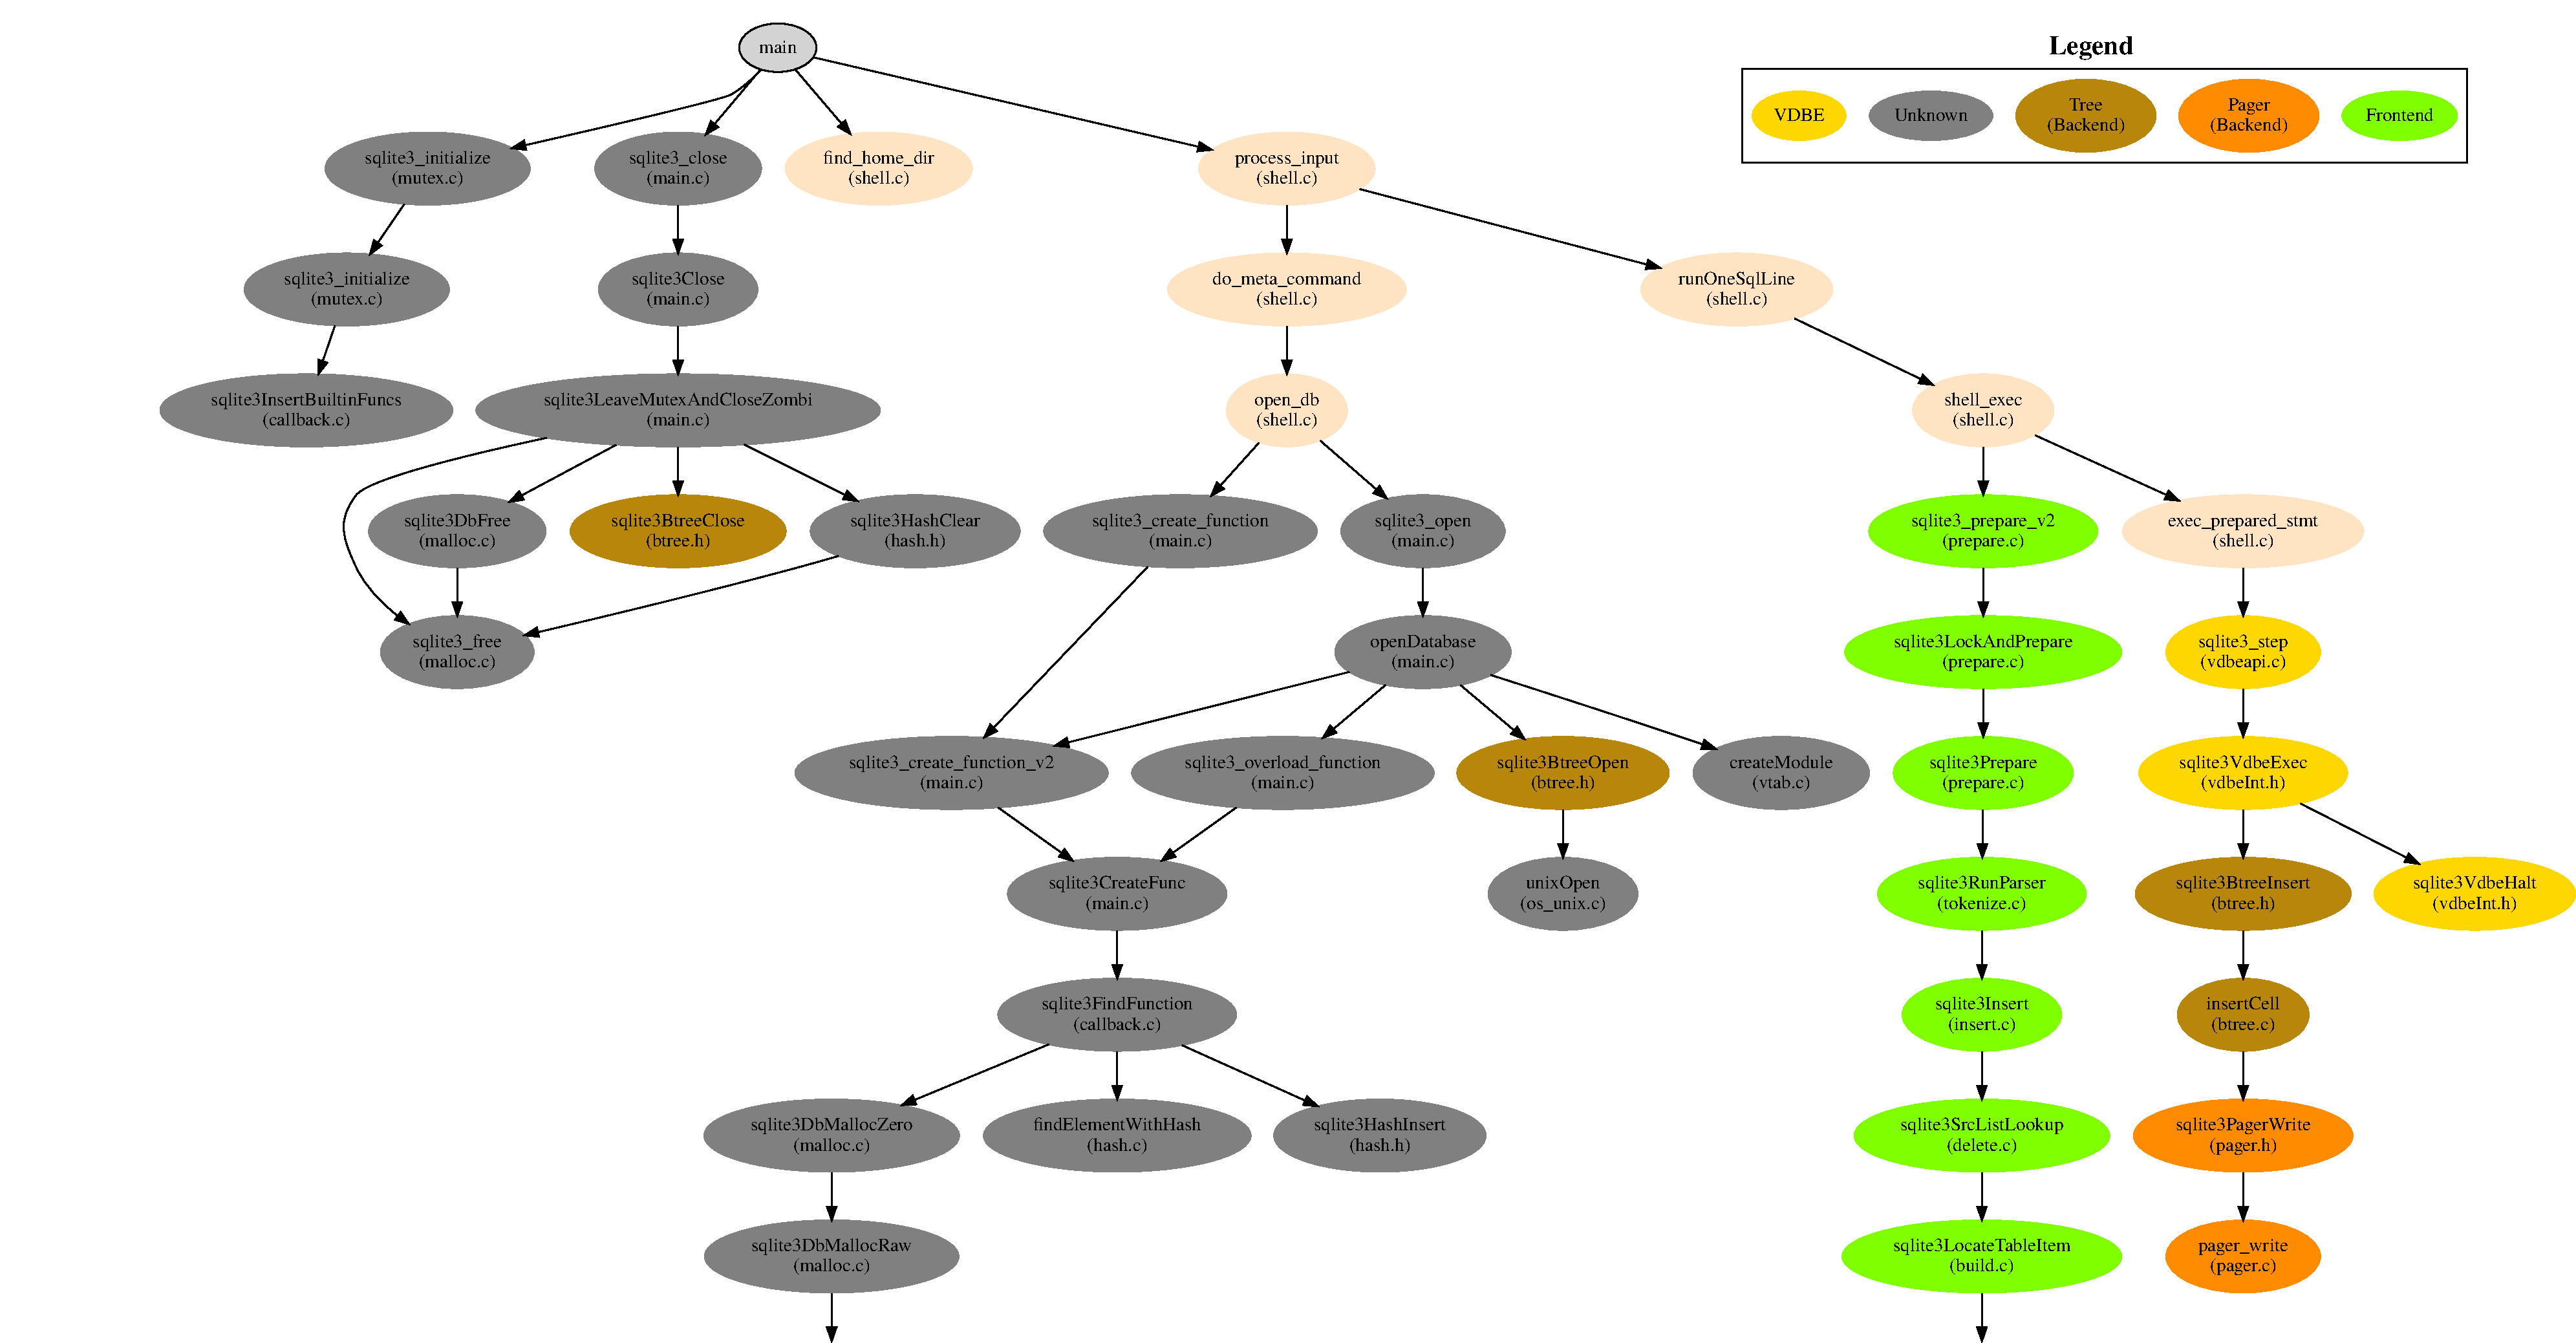
\includegraphics[width=\textwidth]{content/images/sqlite callgraph insert 1percent top.pdf}
\caption{
\textbf{SQLite call graph for insert statement (top half).}\label{ID_450711429}
\label{figure:sqlite-graph}}\end{leftfullpage}\end{sidewaysfigure}
\begin{sidewaysfigure}\begin{fullpage}\ContinuedFloat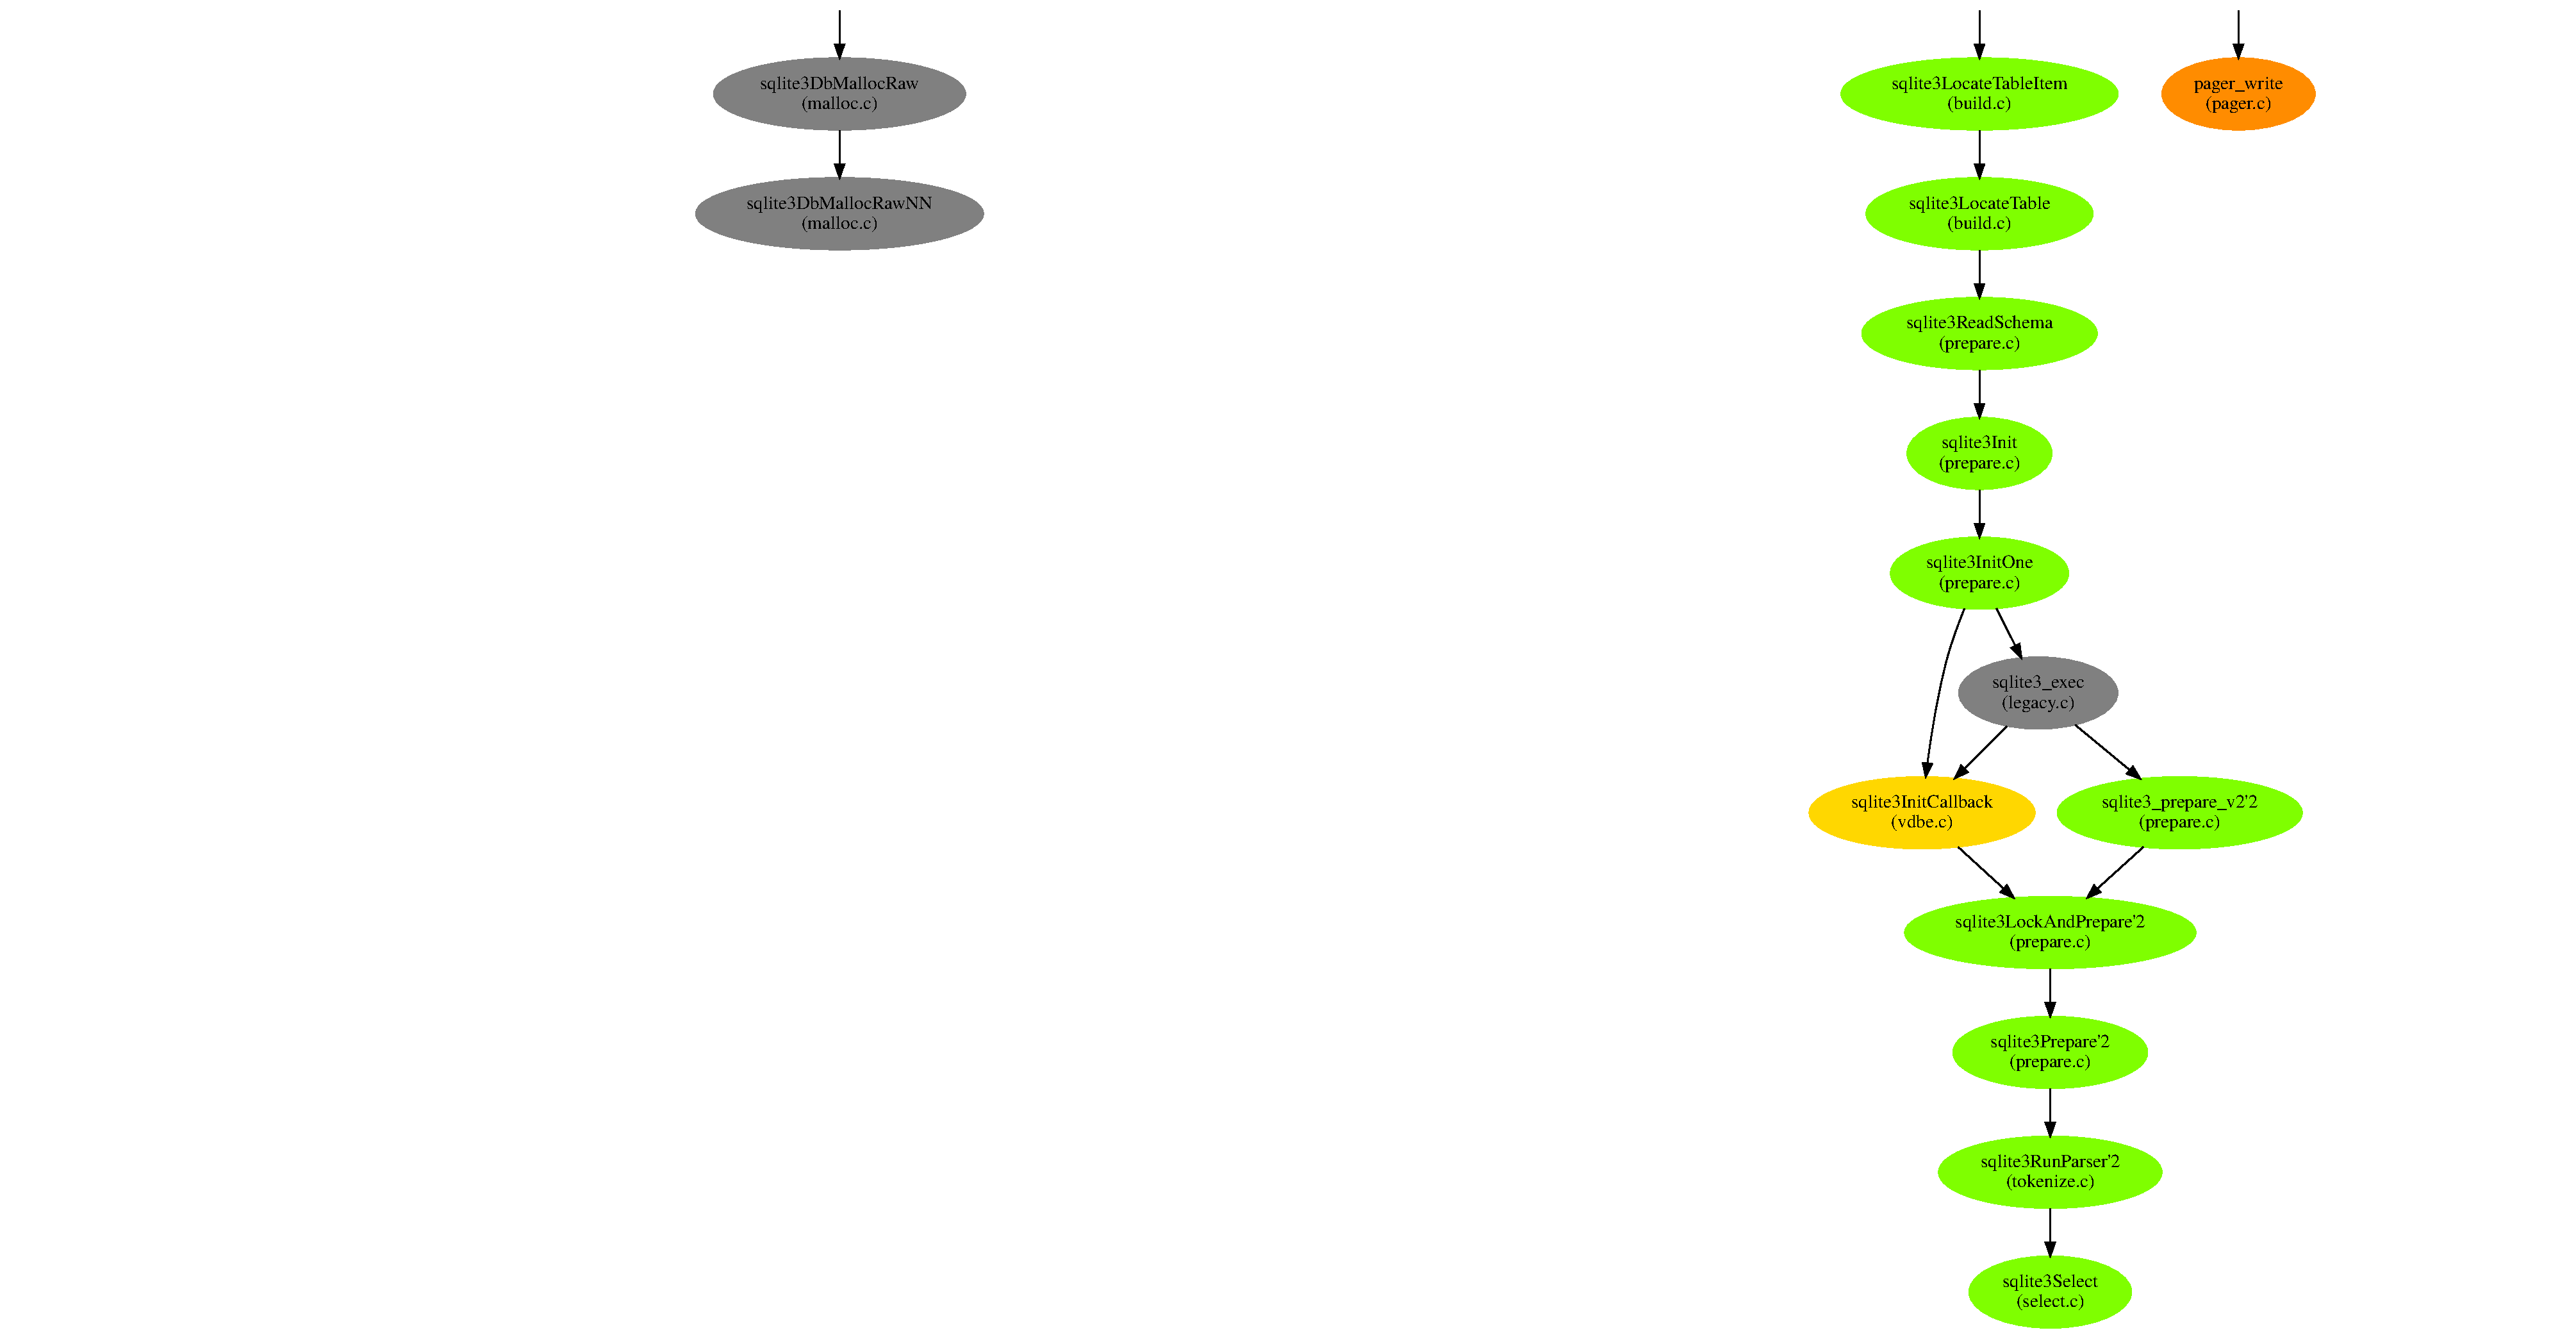
\includegraphics[width=\textwidth]{content/images/sqlite callgraph insert 1percent bottom.pdf}
\caption{
\textbf{SQLite call graph for insert statement (bottom half).}\label{ID_1189342130}
Only function calls (nodes) with a Valgrind cost greater than 1 percent are shown.\label{ID_1717360834}
Nodes are shaded according to the SQLite module they belong to (see the legend).\label{ID_991757666}
The modules are distinguished by the header or code file the function is defined in. The file is given in brackets.\label{ID_189828888}
}\end{fullpage}
\end{sidewaysfigure}
A further visualisation of the same call graph in \autoref{appendix:sqlite} is filtered not by cost, but by depth.\label{ID_489671835}
This is even larger, but can convey an overview of the module interaction through the coloured shading.\label{ID_1179349774}

\section{Concepts\label{ID_207205158}}
Based on the related work and SQLite run time analysis, two different hardening concepts are proposed.\label{ID_806012991}
They are not implemented due to time constraints.\label{ID_946377050}
\begin{enumerate}\label{ID_1303002590}
\item \textbf{Extract the VDBE and tree module into an enclave}.\label{ID_1825072810}
This approach modifies the SQLite code and extracts the security critical part.\label{ID_738821968}
This separates the enclave by functionality (\autoref{section:sgx-hardening}).\label{ID_202493526}
\autoref{figure:sqlite} shows the proposed boundaries of the enclave: it should include the VDBE and tree module.\label{ID_439588279}

The premise is that it is sufficient and secure to protect the VDBE and the tree module.\label{ID_1686599994}
The enclave would provide an interface byte code level. The caller would pass a byte code program in an E-call.\label{ID_5813842}
An in-depth analysis of the data flow is necessary to judge the security implications of this separation.\label{ID_1466004524}

The VDBE executes the compiled byte code program.\label{ID_1148708431}
It fetches entries from the tree module, which in turn access the disk via the pager.\label{ID_770004437}
The tree module is a good lower boundary (in terms of the position in the architecture diagram), because it accesses the disk at the level of pages.\label{ID_1349045404}
The tree module could be adapted to write and read encrypted values, but pass the plain text on to the VDBE.\label{ID_284478389}

The VDBE then performs the actual processing, based on the byte code program.\label{ID_821794728}
It yields individual results row by row to the caller.\label{ID_668651794}
The output has to be encrypted row by row if the interface should remain the same.\label{ID_364110747}
This leaks the number of result rows for every call.\label{ID_999515110}
The VDBE is a good upper boundary, because this keeps the entire front end out of the TCB.\label{ID_311205996}
This is significant, as the code generator alone contains 40 percent of the entire SQLite code.\cite[]{Haldar2015}\label{ID_1881798180}
The front end is not involved in data processing, but only responsible for byte code generation.\label{ID_59920578}

If the byte code is generated by an untrusted front end, it must be ensured that the byte code is not harmful. Also, the output of the VDBE should not leak any information. It should be encrypted to a secure channel established during attestation.\label{ID_902916871}

In reality, the modules are not so well separated as the high-level architecture diagram would have readers believe.\label{ID_109832281}
This can be seen in the call graph (\autoref{figure:sqlite-graph}).\label{ID_1572157209}
Especially calls back and forth between front end and back end are problematic for extracting an enclave.\label{ID_75232381}
While enclaves support O-calls and E-calls, the data that must be passed back and forth is the root of the problem.\label{ID_319109209}
If the untrusted front end must operate on the data it must be passed as plain text, which may break security.\label{ID_1285211358}
\item \textbf{User-defined functions (UDFs) in enclaves}.\label{ID_1233009872}
This solution leaves the KISSDB code base untouched.\label{ID_1587466546}
Instead, sensitive data is processed in enclaves via UDFs.\footnote{Registered via \Q{create_function}: \url{http://www.sqlite.org/c3ref/create_function.html}}\label{ID_321698949}
\autoref{figure:sqlite-udf} shows the architecture of this solution.\label{ID_1839630476}
\begin{figure}[htbp]
\makebox[\textwidth][c]{\begin{tikzpicture}[
	node distance=5pt,
	function/.style={circle, draw, inner sep=2pt, fill=white},
	tt/.style={font=\ttfamily},
]
	\node (udf) at (8,-1.5) {
		UDF enclave
	};
	\node[align=left, below=of udf] (steps) {
		1. decrypt \\
		2. sum \\
		3. encrypt
	};
	
	\begin{scope}[on background layer, shift={(6.5,-4)}]
		\draw[fill=greenbg] (0.25,0.25) rectangle (2.75,3);
	\end{scope}
	
	\node[function,label={[tt]right:secure\_{}sum}] (ss) at (6.5,-0.25) {};
	
	\draw[-latex'] (8,-0.5) -| (8,-1);
	\draw  (6.5,0.75) rectangle (9.5,-4);
	
	\node (sqlite) at (1.5,-1.5) {SQLite};
	
	\matrix [
		below=of sqlite,
        matrix of nodes,row sep=0,
        nodes={anchor=center,rectangle,draw,minimum width=6em, minimum height=12pt, inner sep=0},
	] (hash1) {
	        \textbf{xEnc} & \textbf{yEnc} \\
	        \texttt{4a72c} & {94f2e} \\
	        \ldots & {} \\
	};
	\node[tt] (sql) at (1.5,0.5) {SELECT secure\_{}sum(xEnc,yEnc) FROM tbl};
	\draw  (-1,-1) rectangle (4,-3.75);
	
	\draw[-latex'] (sql) -- (1.5,-1);
	\draw[-latex'] (4,-1.5) -- ++(1.5,0) |- (ss);
	\draw[-latex'] (6.75,-3.25) -- (4,-3.25);
	\node (result) at (1.5,-5) {a29c4};
	\draw[-latex'] (1.5,-3.75) -- (result);
	
	\node at (8,0.25) {UDF};
\end{tikzpicture}

}\caption{\textbf{SQLite hardening with user-defined functions (UDFs)}.\label{ID_1588471613}
A function is registered with a SQLite connection using \texttt{sqlite3\_{}create\_{}function}.\label{ID_1863091039}
The registered function is an untrusted proxy that delegates the call to the enclave.\label{ID_35187670}
The enclave has been provisioned with the encryption key for the data.\label{ID_1543100}
It decrypts the operands and encrypts the result before passing it back.\label{ID_1099637874}
SQLite itself handles only binary encrypted data.\label{ID_326009507}
\label{ID_1287020368}\label{figure:sqlite-udf}}
\end{figure}


The approach is very similar to VC3.\cite[]{Schuster2015}\label{ID_1880634869}
It uses separate processing components (UDFs here, jobs in VC3) which can be plugged into the main processing engine.\label{ID_972553018}
The approach separates enclaves by functionality.\label{ID_653270748}
There is one enclave per UDF.\label{ID_1920750707}

Compared to VDBE and tree extraction, the advantages of the UDF approach are as follows:\label{ID_276876978}
\begin{itemize}\label{ID_1533966412}
\item This approach is far easier to implement.\label{ID_1874885591}
SQLite must not be modified. This facilitates compatibility with future versions.\label{ID_1628619896}
\item The security guaranteed by this approach is easier to reason about, as the data flow is very clear.\label{ID_395790458}
\end{itemize}\label{ID_1825313667}
There are also drawbacks:\label{ID_1006647983}
\begin{itemize}\label{ID_1382823746}
\item Functions have to be re-implemented.\label{ID_34604663}
SQLite has optimised processing implementations. They work well with the tree and pager module. None of these existing operations can be used on encrypted data (for non-homomorphic encryption).\label{ID_680487982}
\item UDFs can only operate at row level.\label{ID_910577627}
Relational operations such as joins will not work if non-deterministic encryption schemes are used.\label{ID_1857752388}
Aggregations can be defined as UDFs (with an interface similar to reducers in functional programming).\label{ID_1002933773}
A combination with the techniques used by other hardened databases in \autoref{section:secure-db} is possible (e.g. onion encryption).\label{ID_1235602590}
\item Performing many E-calls is inefficient.\label{ID_475441213}
Even if the Intel SDK is not used, E-calls still have a performance overhead.\label{ID_141593308}
When processing a query that touches many rows, the enclave will be called many times.\label{ID_907818609}
The resulting context switches into the enclave degrade performance.\label{ID_257744792}
\item Information leakage at the field level.\label{ID_1976381915}
The enclave returns encrypted values.\label{ID_736597701}
However, it is increasingly likely that some information is leaked.\label{ID_1737568991}
If the value space of a field is small or non-uniformly distributed, information may be learned even from an encrypted value (take a binary field with deterministic encryption as an extreme example).\label{ID_1608594282}
\end{itemize}\label{ID_1283973465}
\end{enumerate}\label{ID_852127889}

\section{SQLite in the Intel SGX SDK\label{ID_1312265565}}
The Intel SGX SDK for Linux, which is open source, also includes SQLite.\label{ID_1618983123}
The way in which it is used by enclaves is different to the presented concepts and the related work.\label{ID_1923539167}
For the specific use case of the SDK, it is a simple and interesting alternative.\label{ID_735079837}

Multiple references to SQLite can be found in the SDK's code.\footnote{\url{https://github.com/01org/linux-sgx/search?q=sqlite}}.\label{ID_489883}
Browsing the code, it seems that SQLite is used to provide monotonic counters.\footnote{\url{https://github.com/01org/linux-sgx/blob/1115c195cd60d5ab2b80c12d07e21663e5aa8030/psw/ae/pse/pse_op/monotonic_counter_database_sqlite_rpdb.cpp}}\label{ID_1228268062}
The comments in the repository often mention the CSME, which stands for Converged Security and Manageability Engine.\label{ID_1698867395}
Monotonic counters are provided in hardware by the manageability engine.\cite[]{sgx-windows}\label{ID_106141223}
They are a limited resource.\label{ID_543334142}
SQLite is apparently used to multiplex the hardware monotonic counters into several virtual counters.\label{ID_1316531596}
This is a feature provided by Intel's platform software (PSW).\label{ID_669142565}

The SQLite database is stored outside of the enclaves.\label{ID_1391282}
For the counters, it is sufficient to integrity protect the database.\label{ID_1900027969}
The code indicates that the data is stored in tree form.\label{ID_1206531439}
If stored as a Merkle tree, it is sufficient to securely store the hash of the root node in the enclave.\label{ID_1108434998}
The integrity of the entire tree can be verified from this root hash.\label{ID_635563738}

This approach leaves the payload visible as plain text.\label{ID_719574993}
For the use case, integrity and replay protection are sufficient.\label{ID_1700780161}
This allows for a far simpler solution than the concepts proposed in this case study.\label{ID_207917217}
The SDK approach however falls short of providing protected processing of data, which is the goal of this thesis.\label{ID_1870157400}

\section{Conclusion\label{ID_1290012775}}
In this case study, two concepts to hardening SQLite were proposed.\label{ID_1806868998}
These were based on a brief run-time analysis of SQLite's module interaction.\label{ID_1309249988}
Also, related work provided an inspiration for the UDF approach.\label{ID_402409416}
Due to time constraints, neither of the approaches could be evaluated in-depth or implemented.\label{ID_16617358}
The unrelated approach of the SGX SDK was also presented as an example of storing integrity-protected data outside enclaves.\label{ID_1132675940}

\chapter{Conclusion\label{ID_1572507625}}
This thesis showed how applications can best be hardened with the technology that is available today.\label{ID_1507977384}
In a first step in \autoref{chapter:background}, trusted computing was identified as the correct approach for the type of hardening in mind.\label{ID_580447740}
Alternative approaches based on cryptography alone are either too limited (garbled circuits) or not yet practical (fully homomorphic encryption, encrypted CPU).\label{ID_1382376198}

A major contribution of this thesis is the survey and systematic comparison of trusted computing solutions in \autoref{chapter:tc-solutions}.\label{ID_476358911}
Intel SGX was identified as the best trusted computing technology for hardening applications.\label{ID_1807939320}
The isolated TCB is kept small and the CPU's full processing power can be used.\label{ID_1660655171}
Developers can focus on their application and do not have to provide their own trusted computing infrastructure as on e.g. TrustZone.\label{ID_875938350}

The thesis provided a high-level overview of SGX and summarised criticism and security issues from research in \autoref{chapter:sgx}.\label{ID_517735378}
A helper library for Intel's SDK was developed (\autoref{chapter:sgx-lib}) and made available for public use.\label{ID_381101887}

Architectural design patterns were extracted from related work in \autoref{chapter:related-work}.\label{ID_151365644}
These can be re-used in future work.\label{ID_1282712103}
The case studies (\autoref{chapter:kissdb}, \autoref{chapter:sqlite}) provide a step-by-step template for application hardening.\label{ID_644003251}
The applied reasoning and helper library should prove useful to developers targeting a similar problem.\label{ID_680993229}
Two concepts were derived for the second case study.\label{ID_1182904330}
Implementing one of these approaches is still open work.\label{ID_709376890}
Also, attestation with SGX still has to be explored.\label{ID_34569373}
Only with remote attestation does trusted computing unfold its full potential.\label{ID_1633432001}

This thesis dealt with hardening legacy applications.\label{ID_1399326332}
Intel SGX provides the foundation for entirely new and innovative applications not possible without trusted computing.\label{ID_1610842511}
This line of research has vast potential.\label{ID_1792942181}

Intel has made a serious investment in developing SGX.\label{ID_54424196}
The success of SGX is still far from decided -- too much is still unclear.\label{ID_759430231}
Intel has set itself up in a good position in case SGX succeeds. But judging from the criticism being voiced and the limited amount of applications it may have pushed it's luck too far.\label{ID_971205965}
Further commercial solutions comparable to SGX can be expected to be developed by Intel's competition.\label{ID_1853880623}
Once that time comes, research comparing these solutions will be of interest.\label{ID_1918961193}
Apart from the security aspects and development model, the factor that decides over the winning solution might well be the business model.\label{ID_806891106}
\appendix\label{ID_1376207046}

\chapter{KISSDB Database Files\label{ID_1278383992}\label{appendix:kissdb-files}}
\lstinputlisting[caption={
\textbf{Plain KISSDB database file.}\label{ID_487229369}
The file is shown in hex editor view, with the binary content on the left, and the ASCII characters on the right.\label{ID_1553352177}
Both meta data and payload are in plain text.\label{ID_1172966383}
},style=default,language=hex]{content/listings/kissdb-plaintext-ascii.txt}\label{ID_1976669807}
\lstinputlisting[caption={
\textbf{Hardened KISSDB database file.}\label{ID_934409193}
The file is shown in hex editor view, with the binary content on the left, and the ASCII characters on the right.\label{ID_337106353}
The payload is encrypted, while the meta data is in plain text.\label{ID_85251533}
},style=default,language=hex]{content/listings/kissdb-encrypted-ascii.txt}\label{ID_126877500}

\chapter{SQLite Call Graphs\label{ID_686469438}\label{appendix:sqlite}}
\begin{sidewaysfigure}
\makebox[\textwidth][c]{
	\includegraphics[width=1.1\textwidth]{content/images/sqlite callgraph insert 15callees cropped.pdf}
}\caption{\textbf{SQLite call graph for insert statement.} The depth is limited to a maximum of 15 callees (descendants). The call graph is too large for detailed analysis. Rather, the shading should convey an intuition of how the modules are interleaved. See \autoref{figure:sqlite-graph} for the colour legend. Nodes are coloured according to the SQLite module they belong to (see the legend). The modules are distinguished by the header or code file the function is defined in. The file is given in brackets.\label{ID_196264389}\label{ID_196264389}}
\end{sidewaysfigure}





	% ggf. Anhang
	\appendix\include{content/appendix} % example

	% Bibliographie
	\addcontentsline{toc}{chapter}{\refname}
	\printbibliography

	% Eigenständigkeitserklärung
	\ifisbook\pagestyle{plain}\cleardoubleemptypage% => Laut Aussage des Studienreferats braucht es - auch wenn die Arbeit in englischer Sprache verfasst ist - KEINE separate Version der Eigenständigkeitserklärung auf Englisch. Sowohl für Arbeiten in deutscher Sprache als auch für Arbeiten in englischer Sprache genügt EINE EINZIGE Eigenständigkeitserklärung auf DEUTSCH.
\begin{otherlanguage}{ngerman}

\begin{center}\textsf{\textbf{Eidesstattliche Erklärung}}\end{center}
Hiermit versichere ich, dass meine {\hpitype} \enquote{\hpititle} (\enquote{\hpititleother}) selbständig verfasst wurde und dass keine anderen Quellen und Hilfsmittel als die angegebenen benutzt wurden. Diese Aussage trifft auch für alle Implementierungen und Dokumentationen im Rahmen dieses Projektes zu.\\

\noindent
Potsdam, den \hpidate,
\vspace{2cm}

\begin{center}
\begin{tabular}{C{6cm}}
\hline
{\small({\hpiauthor})}
\end{tabular}
\end{center}

\end{otherlanguage}


\fi

\end{document}
